% !TEX TS-program = pdflatexmk
% !TEX spellcheck = language_tag
\documentclass[fleqn,usenatbib]{mnras}

\usepackage[T1]{fontenc}
\usepackage{ae,aecompl}

\usepackage{graphicx}
\usepackage{amsmath}
\usepackage{amssymb}
\usepackage{newtxtext,newtxmath}

\usepackage{multirow}
\usepackage{array}
\usepackage{xcolor}
\usepackage{ulem}
\usepackage{xspace}
\usepackage[abs]{overpic}
\usepackage{pict2e}

% ABBREVIATIONS
\newcommand{\ud}{\ensuremath{\mathrm{d}}\xspace}
\newcommand{\tpb}{\ensuremath{t_{\text{pb}}}}

\newcommand{\helium}{\ensuremath{\mathrm{^{4}He}}\xspace}
\newcommand{\nickel}{\ensuremath{\mathrm{^{56}Ni}}\xspace}
\newcommand{\tracer}{\ensuremath{\mathrm{Tr}}\xspace}
\newcommand{\ye}{\ensuremath{Y_{e}}\xspace}
\newcommand{\iron}{\ensuremath{\mathrm{^{56}Fe}}\xspace}
\newcommand{\cobalt}{\ensuremath{\mathrm{^{56}Co}}\xspace}

\newcommand{\solr}{\ensuremath{\rm{R_{\odot}}}\xspace}
\newcommand{\solm}{\ensuremath{\rm{M_{\odot}}}\xspace}
\newcommand{\mns}{$M_{\mathrm{NS}}$}
\newcommand{\rsh}{$R_{\text{s}}$}
\newcommand{\rrevsh}{$R_{\mathrm{revs}}$}
\newcommand{\rgain}{$R_{\mathrm{gain}}$}

\newcommand{\kms}{\ensuremath{\mathrm{km\, s^{-1}}}}
\newcommand{\km}{\ensuremath{\mathrm{km}}}
\newcommand{\s}{\ensuremath{\text{s}}}
\newcommand{\ms}{\ensuremath{\text{ms}}}
\newcommand{\gcc}{\text{g}\, \text{cm}^{-3}}
\newcommand{\kbpnuc}{k_{\text{b}}/\text{nucleon}}


\newcommand{\prom}{\textsc{Prometheus-HOTB}\xspace}
\newcommand{\vertexprom}{\textsc{Vertex-Prometheus}\xspace}
\newcommand{\vertex}{\textsc{Vertex}\xspace}
\newcommand{\nada}{\textsc{NADA-FLD}\xspace}
\newcommand{\rns}{\ensuremath{R_{\mathrm{NS}}}\xspace}

\newcommand{\onemg}{\ensuremath{\mathrm{e8.8}}\xspace}
\newcommand{\snine}{\ensuremath{\mathrm{s9.0}}\xspace}
\newcommand{\znine}{\ensuremath{\mathrm{z9.6}}\xspace}

%keeping track of changes
\newcommand{\NY}[2]{{\color{blue}\sout{#1}#2}}
\newcommand{\GEO}[1]{{\color{red}#1}}
\newcommand{\COM}[1]{{\color{orange}#1}}

\title{Three-dimensional Models of Core-collapse Supernovae From Low-mass Progenitors}

\author[G. Stockinger et. al]{
 G.~Stockinger$^{1,2}$\thanks{Email: georgsto@mpa-garching.mpg.de},
 H.-T.~Janka$^1$,
 T.~Ertl$^1$,
 D.~Kresse$^1$,
 K.~Nomoto$^3$,
 A.~Tolstov$^3$,\and
 S.~Leung$^4$,
 A.~Heger$^{5,6,7}$,
 A.~Gessner$^8$
 \\
% Institutions
$^1$Max Planck Institute for Astrophysics, Karl-Schwarzschild-Str.1 , D-85748 Garching, Germany\\
$^2$Physik Department, Technische Universit\"at M\"unchen, James-Franck-Stra{\ss}e 1, D-85748 Garching, Germany\\
$^3$Kavli Institute for the Physics and Mathematics of the Universe (WPI), The University of Tokyo Institutes for Advanced Study,\\  \hspace{0.08cm} The University of Tokyo, Kashiwa, Chiba 277-8583, Japan\\
$^4$Department of Physics, the Chinese University of Hong Kong, Hong Kong S. A. R., China \\
$^5$School of Physics \& Astronomy, University of Minnesota, Minneapolis, MN-55455, USA \\
$^6$Center for Nuclear Astrophysics, Department of Physics \& Astronomy, Shanghai Jiao-Tong University, Shanghai-200240, P. R. China \\
$^7$Joint Institute for Nuclear Astrophysics, 1 Cyclotron Laboratory, National Superconducting Cyclotron Laboratory, Michigan State University,\\ \hspace{0.08cm} East Lansing, MI-48824-1321, USA \\
$^8$Max Planck Institute for Intelligent Systems, Max-Planck-Ring 4, D-72076 T\"ubingen, Germany \\
}

\date{Released 2019 Xxxxx XX}

% Enter the current year, for the copyright statements etc.
\pubyear{2019}
\hypersetup{draft}
\begin{document}
\label{firstpage}
\pagerange{\pageref{firstpage}--\pageref{lastpage}}
\maketitle
\pubyear{2019}

\begin{abstract}
We present the results of full $4\pi\mathord{-}$3D, long-time simulations 
of core-collapse supernovae (CCSNe) resulting from low-mass progenitors, 
covering the evolution from bounce through shock revival until shock breakout. 
We consider two low-mass iron core progenitors of 9.6 \solm and 9.0 \solm 
with zero metallicity and solar metallicity, respectively, and one 
progenitor with an oxygen-neon-magnesium core, which explodes as an 
electron-capture supernova (ECSN). In the ECSN case, mixing of nickel is 
inefficient because of a relatively spherical beginning of the explosion, 
triggered by a steep density gradient outside of the degenerate core and 
the concomitant absence of secondary non-radial instabilities at 
composition-shell interfaces of the progenitor. The similarity between the 
core structure of the zero-metallicity progenitor and the ONeMg progenitor 
leads to similarities in their explosion properties. In both of these cases, 
we observe roughly equal amount of nickel mixing in mass and velocity space 
and qualitatively similar ejecta morphology at late times, characterized by 
small deviations from spherical symmetry. In contrast, the solar-metallicity 
iron core progenitor explosion shows strong growth of Rayleigh-Taylor plumes 
in the entire helium core. The large initial asymmetries lead to more 
pronounced mixing. In this case the final morphology is remarkably similar 
to the remnant morphology seen in long-time simulations of massive progenitors. 
Interestingly, the shock deceleration in the extended hydrogen envelope of 
this model is so extreme that a fast nickel plume catches up with the 
shock and leads to shock deformation and an aspherical breakout of the 
shock at the stellar surface.
\end{abstract}

\begin{keywords}
  supernovae: general -- stars: massive -- stars: neutron
\end{keywords}

\noindent

\section{Introduction}

According to current understanding stars with masses 
$\mathord{\gtrsim}\,8\, \solm$ end their lives in a core-collapse 
supernova. The explosion is powered by gravitational energy, 
which is released when the core of the star collapses to a compact 
remnant (a neutron star or black hole). In the past six decades 
numerous studies have focused on the collapse phase and subsequent 
evolution using 1D simulations. Over the past two decades, 
multi-dimensional simulations with successively improved treatment 
of the microphysics have driven our understanding of the core-collapse 
problem (see e.g. \citealt{Janka2012,Burrows2013,Janka2016}). 
A close study of these models led to the discovery of new hydrodynamic 
instabilities such as the standing accretion shock instability (SASI) 
(\citealt{Blondin2003,Foglizzo2007}). The increase in computational 
capabilities in the recent years along with new developments in 
neutrino transport methods (see e.g. 
\citealt{Buras2006,OConnor2018,Skinner2019,Glas2019} and references therein)
has enabled full 3D simulations (see e.g. 
\citealt{Melson2015a,Summa2016,Mueller2017,Mueller2018,Vartanyan2018,Melson2019,Vartanyan2019}). 
Motivated by the historical SN1987A and its progenitor detection, a 
variety of studies also investigated the propagation of the shock 
wave from its initiation, firstly by artificial energy deposition 
at the center (see e.g. \citealt{Mueller1991}), later by the 
neutrino-driven mechanism (see \citealt{Kifonidis2003,Hammer2010,Wongwathanarat2015}), 
to the breakout of the shock from the stellar surface in 15-20 $\solm$ models, 
which are suitable as progenitors for SN1987A, in two and three dimensions. 
Also the long-time evolution of the explosion of ultra-stripped 
progenitors was investigated by \cite{Mueller2018}, due to their 
importance in understanding the origins of the recent detection of 
NS-NS mergers by Ligo/VIRGO (GW170817, \citealt{Abbott2017}).

These theoretical works showed that supernova explosions are by far 
not spherical events as previously thought. Three-dimensional 
instabilities facilitate explosions 
\citep{Herant1994a,Burrows1995,Janka1996,Melson2015a,Mueller2017} 
and are a necessary ingredient to explain the clumpiness and 
mixing found in photospheric emission \citep{Utrobin2015,Utrobin2017} 
and spectral analyses of the nebular phase of core-collapse events \citep{Jerkstrand2017}. 
\citet{Wongwathanarat2015} showed that the final ejecta 
distribution carries imprints of the 
asphericities produced during the onset of the explosion 
($t\,\mathord{\sim}\, 1\, \rm s$), which are further modified during 
later phases. Depending on the detailed progenitor structure, hydrodynamic 
instabilities arising at the composition interfaces, such as the Rayleigh-Taylor 
instability (RTI) and the Richtmeyer-Meshkov instability (RMI), shapes 
the final spatial and velocity distribution of nucleosynthetic products. 
The resulting ejecta morphology exhibits inhomogenously mixed ejecta and 
strongly pronounced RT-fingers resembling also the geometry found in Cas A 
\citep{Wongwathanarat2017,Grefenstette2017}. Due to the highly complex and 
stochastic behaviour of nonradial instabilities and turbulence during the 
onset of the explosion phase and the nonlinear evolution of the RTI, a clear 
connection between the asymmetries, and thus the degree of mixing, and 
the progenitor structure has still to be worked out.

In this paper we consider CCSN progenitors with masses near the low 
mass end of about 9 \solm - 10 \solm, where up to 40\% of all CCSNe 
are thought to occur (assuming a Salpeter initial mass function  
\citep{Salpeter1955} and an upper mass limit of $\mathord{\sim}20\,\solm$ 
for CCSNe), to study the differences in their development of mixing 
instabilities during the explosion. To this end we compare 
electron-capture SNe (ECSNe) from ONeMg core progenitors and 
CCSNe from iron care progenitors, all with around $9\,\solm$. 

The evolution of stars with masses $\mathord{\lesssim}\,12\, \solm$ 
is very sensitive to the initial stellar mass and various 
pulsational instablities and mass-loss phenomena \citep{Woosley2015}.
iron core CCSN progenitors with masses around $9\mathord{-}10\,\solm$ 
ignite oxygen burning off-center in contrast to their more massive 
($M \mathord{>} 15\, \solm$) counterparts. After oxygen burning, silicon 
ignites in a degenerate flash which can, in some cases, lead to 
additional mass loss in the last decade of evolution or even to 
ejection of the hydrogen envelope \citet{Woosley2015}.

The $8.8\, \solm$ progenitor of \cite{Nomoto1984} is even more peculiar. 
It experiences  several thermal pulses and off-center ignition of 
fusion material. In the end, it has a degenerate ONeMg core 
surrounded by a dilute and an extended hydrogen envelope.
 
When the core approaches its Chandrasekhar mass electron captures 
on $\mathrm{^{24}Mg}$ via the reactions 
$\mathrm{^{24}Mg(e^-,\nu_e)}^{24}\mathrm{Na}$ and 
$\mathrm{^{24}Na(e^-,\nu_e)}^{24}\mathrm{Ne}$ \cite{Miyaji1980} 
destabilize the core due to the reduction of the effective 
adiabatic index of the electron-degeneracy dominated gas pressure. 
Continuous $e^-$-capture on $\mathrm{^{20}Ne}$, which further 
reduces the pressure support, works against the now beginning 
oxygen-burning as temperatures increase during the collapse. 
Simulations in 1D (see e.g. \citealt{Kitaura2006,Janka2008,Fischer2010}) 
suggest that the collapse proceeds despite the oxygen burning. 
\cite{Jones2016} simulated the deflagration of oxygen in ONeMg 
cores with different core densities. Below $\log_{10}\rho_c=10.3$ 
their cores do not collapse but get partly unbound due to the inefficient 
semi-convective mixing during the electron capture phase and the 
resulting strong thermonuclear runaway. Only when central densities 
are higher than this threshold value of $\rho_c$ the core is 
found to collapse to a proto-neutron star (PNS).
Recently, \cite{Kirsebom2019} investigated the influence of a newly 
measured rate of a strong transition between the ground states of 
$^{20}\mathrm{Ne}$ and $^{20}\mathrm{F}$ on the evolution of ONeMg 
cores. Adding the new transition increases the likelihood that the 
star is (partially) disrupted by a thermonuclear explosion (termed tECSN) 
rather than collapsing to form a PNS. 
In this study, however, we assume the collapse of the ONeMg core to a 
PNS leading to a ``collapse ECSN'' (cECSN) as recent studies 
covering the galactic chemical evolution of the galaxy stress 
their importance to reproduce the solar abundances of several 
important and problematic isotopes including e.g. 
$\mathrm{^{48}Ca}$, $\mathrm{^{50}Ti}$ and several of the 
$\mathrm{Zn}–\mathrm{Zr}$ isotopes \cite{Jones2019}.

Despite the narrow range of central densities at which 
cECSNe occur \cite{Leung2019} and competing processes that 
depend strongly on the employed physics, observations of 
ECSNe have been made in connection with SN 1994N, 1997D, 
1999br, 1999eu, 2011dc and 2005cs \citep{Stevenson2014}. Also 
SN1054 (the Crab) has been speculated to be an ECSN although it 
is in conflict with results by \cite{Gessner2018} for the maximum 
kick velocity of PNSs produced by ECSNe.

In this work we attempt to investigate the following questions
with the help of fully three-dimensional simulations:

\begin{itemize}

\item What are the differences in the initiation of the 
explosion of low-mass Fe-core end ONeMg-core progenitors?

\item What is the influence of each progenitor structure on 
the long-time evolution of the explosion? In particular, what 
is the influence on the formation of reverse shocks and the 
efficiency of mixing of neutrino-heated material?

\item Are low-mass progenitors of CCSNe able to produce highly 
mixed ejecta in a similar fashion as their more massive 
counterparts as found in previous studies?

\end{itemize}

\section{Progenitors}
% pre collapse 
In this paper, we study an ECSN of a non-rotating 8.8 \solm 
progenitor (\onemg) \citetext{Nomoto, 2017, private communication} 
and two non-rotating CCSNe resulting from low-mass iron core progenitors 
(\znine, \snine), provided by A. Heger \citetext{2015, private communication} 
and \cite{Woosley2015}, respectively. The considered ECSN 
progenitor is explored here for the first time, whereas the 
explosions of the iron core progenitors were simulated in 3D 
with the \vertexprom code and some results were published in 
\cite{Melson2015a} and \cite{Melson2019}.

\subsection{ONeMg-core progenitor}
Model \onemg is a solar-metallicity progenitor with a ZAMS mass of 
$M_{\rm ZAMS}\mathord{=}8.8\,\solm$ and was provided by Nomoto 
\citetext{2017, private communication}. This progenitor has an ONeMg 
core that explodes as an ECSN. 
It has the typical very sharp density gradient outside of its $1.33\, \solm$ 
ONeMg core ($\xi_{2.5}\mathord{=}5.7\times10^{-6}$, $\xi_{1.5}\mathord{=}8.0\times10^{-6}$)
\footnote{Because of its relevance for higher-mass progenitors we provide the 
compactness parameter \citep{OConnor2011} 
{$\xi_{M}\equiv \frac{M/\solm}{R(M_{\rm bary}\mathord{=}M)/10^{3}\, \rm km}$}. 
Due to the steep density gradient outside of the core of the considered progenitors, 
its relevance in the present context is, however, questionable.} which can 
be seen from the density ($\rho$) profile in Figure~\ref{fig:prog_tem_rho_ye_rhor}, 
where we also show the $\rho r^3$-profiles, besides the electron fraction 
$Y_{\mathrm{e}}$ and temperature $T$ as functions of enclosed mass and radius. 
The dash-dotted, dashed and dotted lines indicate the positions of the degenerate 
core/CO, CO/He and He/H composition interfaces, respectively. 
\GEO{We define the locations of the composition interfaces, similar to 
\cite{Wongwathanarat2015}, as those positions at the bottom of the respective 
layers of the star where the mass fractions $X_{i}$ drop below half of their 
maximum values in the layer. The radial positions of the composition 
interfaces are summarized in Table~\ref{tab:progenitors}.}
In the top panel of Figure~\ref{fig:composition_all} we present the 
composition of model \onemg, where we combine all elements with mass 
numbers greater than 28 into ``iron-group'' (IG) material or nuclei
in nuclear statistical equilibrium (NSE).
The ONeMg-core is surrounded by very thin carbon and helium shells 
($M_{\rm C}\,\mathord{\approx}\, 8.1\mathord{\times}10^{-3}\, \solm$, 
$M_{\rm He}\,\mathord{\sim}2.1\mathord{\times}\,10^{-6}\, \solm$) and a 
hydrogen ($\mathrm{H}\mathrm{+}\mathrm{He}$) 
envelope ($M_{\rm H}\,\mathord{\approx}\, 4.49\, \solm$).  

A previous version of the progenitor \citep{Nomoto1984,Nomoto1987,Nomoto2008}, 
commonly termed \onemg in the literature and $\mathrm{e}8.8_{\mathrm{n}}$ 
in this publication, has been used in various studies, including 
nucleosynthesis \citep{Wanajo2018} and PNS kicks \citep{Gessner2018} and 
is a reference case for supernova simulations of ECSNe. The previously used 
progenitor $\rm e8.8_{\mathrm{n}}$ has a more massive helium core with 
a mass of $\mathord{\sim} 1.375 \,\solm$ (compared to $\mathord{\sim}1.34\solm$), 
but a smaller hydrogen envelope (see Figure~\ref{fig:prog_tem_rho_ye_rhor}). 
The collapse and post-bounce 
evolution of the new progenitor are computed with \prom as detailed 
in Section~\ref{sec:Collapse and post-bounce setup in prom}.

\subsection{Fe-core Progenitors}
As a second progenitor we employ a zero-metallicity 
$M_{\text{ZAMS}}\mathord{=}9.6\,\solm$ star, termed \znine. 
It was first used by \citet{Janka2012} and is also considered in other 
studies such as \citet{Mueller2013,Mueller2018}. This iron core 
progenitor is structurally similar to the ECSN model. It also shows a 
sharp decline of the density at the edge of its iron core, enabling low-energy 
explosions in 1D \citep{Melson2015}. 
Evolved as an extension to \cite{Heger2010}, the pre-SN model develops an 
iron core of about 1.30 \solm. The iron core is surrounded by a $0.061\,\solm$ 
Si-layer, a $0.016\,\solm$ CO-layer, and has a helium layer of about 0.33
\solm below a massive hydrogen envelope of $\mathord{\sim}8$ \solm 
($\xi_{2.5}\mathord{=}7.65 \times 10^{-5}$, $\xi_{1.5}\mathord{=}2.37 \times 10^{-4}$).
As the envelope is not enriched by metals, mass loss played only a negligible 
role during the star's evolution. This leaves the total mass of the star 
almost unchanged (see Table~\ref{tab:progenitors}). 
Due to its structure it was one of the first iron core progenitors that exploded 
in fully self-consistent 3D simulations by \cite{Melson2015a} with \vertexprom. 
This result provides the initial state for our investigation. 

Moreover, we investigate a solar-metallicity $M_{\text{ZAMS}} \mathord{=} 9.0 \,\solm$ 
star, termed \snine, of \citet{Sukhbold2016}. Its 1.30 \solm iron core is 
surrounded by a silicon shell of 0.03 \solm, a carbon-oxygen layer of 0.068 
\solm and a helium shell of 0.169 \solm (see Table~\ref{tab:progenitors}). 
The hydrogen envelope extends from 1.57 \solm up to 8.75 \solm 
($\xi_{2.5}\mathord{=}3.83 \times 10^{-5}$, $\xi_{1.5}\mathord{=}5.25 \times 10^{-3}$).
This progenitor was chosen to be representative for low-mass CCSNe 
by \cite{Jerkstrand2018}, who focused on the late-time nebular spectra 
of the supernova, and by \cite{Glas2019} focusing on the neutrino 
emission during the explosion. The three-dimensional exploding model for 
our investigation is provided by \citet{Melson2019} and has also been 
modeled with \vertexprom. 

Although the progenitors considered in this study have very 
similar ZAMS masses, 
their pre-collapse core structures differ strongly 
(see Figure~\ref{fig:prog_tem_rho_ye_rhor}).
We stress the importance of the $\rho r^3$-profiles of the progenitors as 
they are decisive for the overall evolution of the explosion 
\citep{Kifonidis2003,Wongwathanarat2015}. 
The behavior of the $\rho r^3$-profile yields important information on 
the propagation of the shock through the stellar structure because, 
according to \cite{Sedov1961}, positive gradients of $\rho r^3$ cause 
shock deceleration, whereas negative gradients cause the opposite. 
Additionally, variations of the shock velocity produce crossing 
pressure and density gradients behind the shock front near the 
composition-shell interfaces \citep{Chevalier1978}. 
Such conditions are essential for 
Rayleigh-Taylor instabilities as detailed in 
Section~\ref{sec:Linear stability analysis}, assigning them a 
crucial role for explaining the high-velocity metal-rich ejecta 
and the radial mixing of heavy elements 
\citep{Arnett1989,Nomoto1990,Wongwathanarat2015}.

The ECSN progenitor exhibits an extremely sharp drop of the 
$\rho r^3$-profile just outside of the ONeMg core. It is this drop 
in density that enables fast explosions due to an early, rapid drop 
of the mass accretion rate and of the corresponding ram pressure at the 
SN shock \citep{Kitaura2006}. Outside the core, the $\rho r^3$-profile 
grows monotonically as no other composition interfaces are encountered.
The \znine progenitor falls into the class of ECSN-like progenitors also 
in this respect: Similar to the electron-capture progenitor, the \znine
model shows a monotonic growth of the $\rho r^3$-profile outside the CO 
core, where only a small step in the density profile can be seen at the 
He/H interface.
Model \snine on the other hand exhibits strong variations in its 
$\rho r^3$-profile. Shells of different composition are clearly separated 
by a negative $\rho r^3$-gradient just before the respective interface. Of 
particular interest are the CO/He and He/H interfaces. These will have an 
impact on the long-time evolution of the explosion as will be discussed 
in Section~\ref{sec:Linear stability analysis}.

\begin{figure*} % FIGURE 1
 \centering
 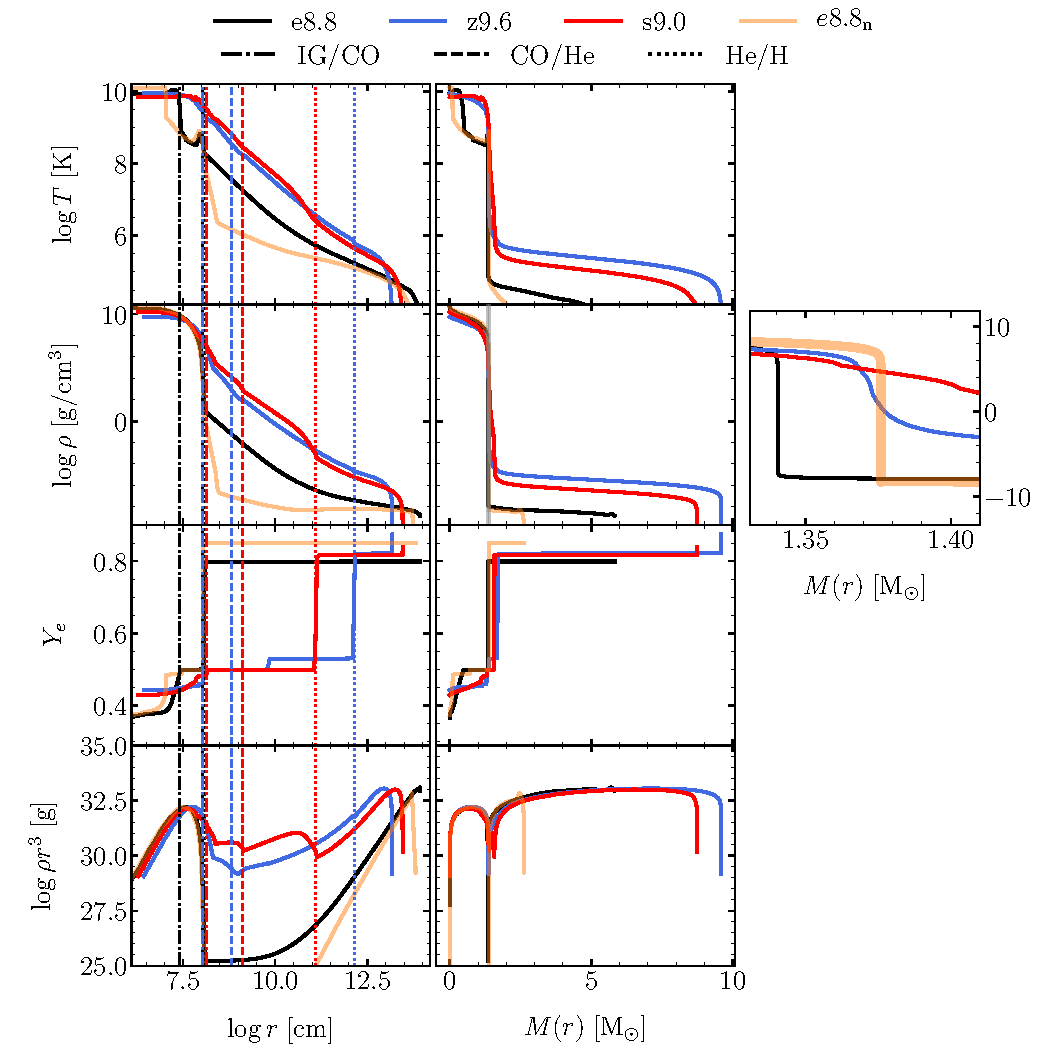
\includegraphics[width=0.9\textwidth,trim=1cm 0.0cm 1cm 0cm]{./pic/progenitors_tem_rho_ye_rhor_paper.pdf}
 \caption{Profiles of the temperature, density, electron 
 fraction ($Y_{\text{e}}$) and $\rho r^3$ for the progenitor 
 models as functions of radial coordinate (left panels) and mass 
 coordinate (right panels). Indicated by dash-dotted, dashed and 
 dotted lines are the outer boundaries of the degenerate 
 (iron or NSE), CO and He 
 cores, respectively. Note the huge differences in the density 
 and $\rho r^3$-profiles between the progenitors with iron 
 and ONeMg cores in particular just outside the CO core. 
 We show the difference in the 
 core structure of our ONeMg core models as a zoom in the $\rho$ vs $M(r)$
 profiles in the rightmost panel.}
 \label{fig:prog_tem_rho_ye_rhor}
\end{figure*}

For this paper we performed spherically symmetric (1D), 
axisymmetric (2D) and fully three-dimensional (3D) 
simulations for all progenitors until the shock reaches 
the surface of the star. The different setups and approaches 
for the simulations will be described in the following section.
\begin{figure*} % FIGURE 2
 \centering
 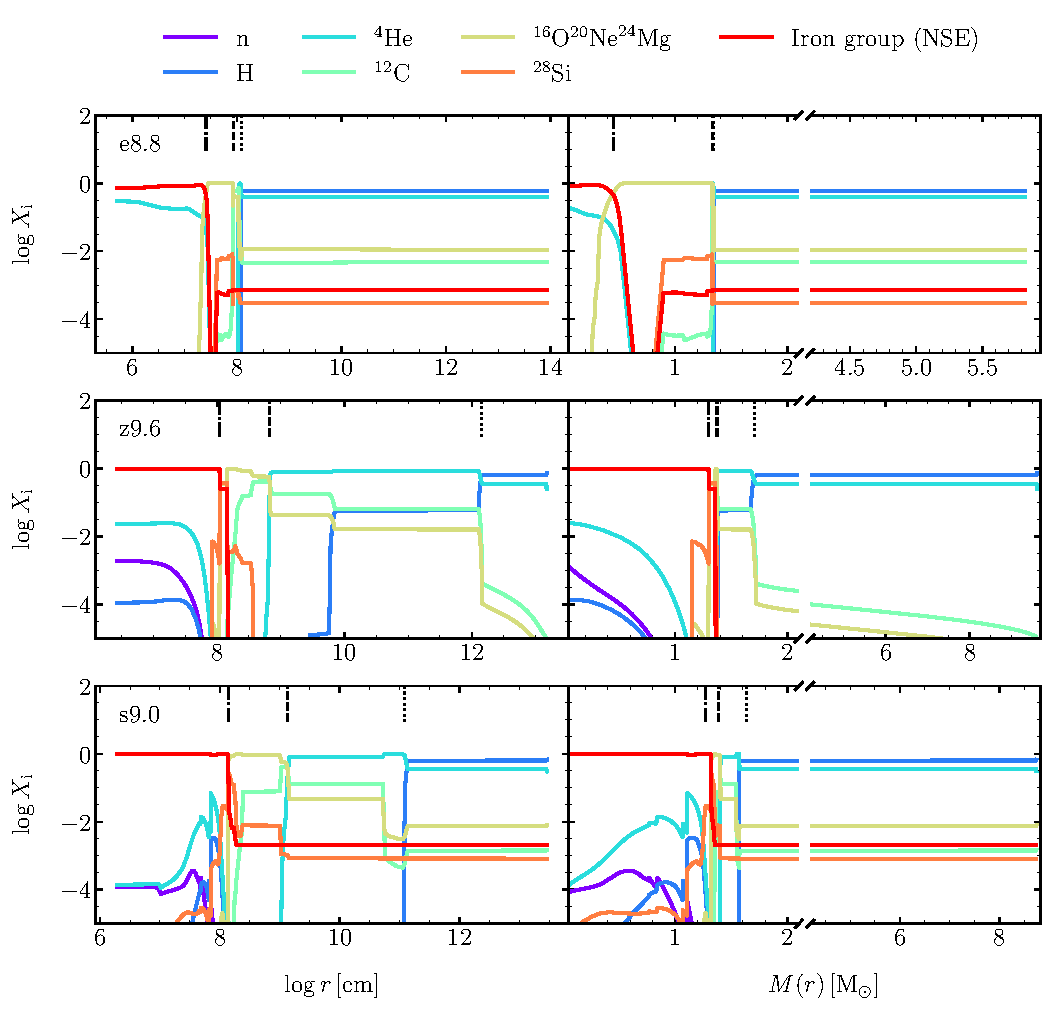
\includegraphics[width=0.9\textwidth,trim=0cm 0.0cm 0cm 0cm,clip]{./pic/composition_all.pdf}
 \caption{Initial pre-collapse composition of models 
 \onemg (top), \znine (middle) and \snine (bottom) as a function 
 of radius (left) and enclosed mass (right). We combine all elements 
 with mass numbers greater than 28 into the ``iron-group'' (IG). The 
 dash-dotted, dashed and dotted lines indicate the the outer 
 boundaries of degenerate (iron or NSE), CO and He cores, respectively.}
 \label{fig:composition_all}
\end{figure*}

\begin{table*}
   \caption{Shell structure of the pre-collapse progenitor models.}
   \label{tab:progenitors}
   \begin{tabular}{l l l l l} 
   \hline
     Model      &Interface & $\mathrm{R_{shell}\,}$ & $\mathrm{M_{shell}}$ & $t_{\mathrm{sh}}^{\mathrm{3D}}$\\ [0.5ex] 
                &          & [cm] & $[\solm]$ & $[\s]$\\ [0.5ex] 
   \hline
   \multirow{5}{*}{\onemg} & IG/ONeMg & $2.57\mathord{\times} 10^{7}$  & 0.45 & - \\ 
                           & ONeMg/C  & $8.48\mathord{\times} 10^{7}$  & 1.33 & 0.15 \\
                           & C/He     & $1.09\mathord{\times} 10^{8}$  & 1.34 & 0.17 \\
                           & He/H     & $1.21\mathord{\times} 10^{8}$  & 1.34 & 0.18\\
                           & Surface  & $8.43\mathord{\times} 10^{13}$ & 5.83 & $4.1\mathord{\times}10^5$\\
   \hline
   \multirow{5}{*}{\znine} & IG/Si    & $1.10\mathord{\times} 10^{7}$  & 1.30 & 0.09 \\ 
                           & Si/CO    & $1.45\mathord{\times} 10^{7}$  & 1.36 & 0.11\\ 
                           & CO/He    & $6.73\mathord{\times} 10^{8}$  & 1.37 & 0.40\\
                           & He/H     & $1.40\mathord{\times} 10^{12}$ & 1.70 & $1.7\mathord{\times}10^{3}$\\
                           & Surface  & $1.50\mathord{\times} 10^{13}$ & 9.60 & $1.2\mathord{\times}10^5$  \\
   \hline
   \multirow{5}{*}{\snine} & IG/Si    & $1.24\mathord{\times} 10^{7}$  & 1.30 & 0.08 \\ 
                           & Si/CO    & $1.55\mathord{\times} 10^{7}$  & 1.33 & 0.30 \\ 
                           & CO/He    & $1.34\mathord{\times} 10^{9}$  & 1.40 & 1.30\\
                           & He/H     & $1.21\mathord{\times} 10^{11}$ & 1.57 & 124.0 \\
                           & Surface  & $2.86\mathord{\times} 10^{13}$ & 8.75 & $3.2\mathord{\times} 10^5$ \\
  \hline
   \end{tabular}

\flushleft
\textit{Notes}: The radii of the composition interfaces, $\mathrm{R}_{\mathrm{shell}}$,
are defined as those positions at the bottom of the stellar layers (e.g. CO)
where the mass fractions (e.g. C+O) drop below half of their maximum values 
in the respective layer first. We also show the mass $\mathrm{M}_{\mathrm{shell}}$ 
contained within the corresponding radius and the post-bounce time 
when the outermost radius of the
forward shock of our three-dimensional models reaches the interface.
\end{table*}


\section{NUMERICAL METHODS AND PHYSICAL SETUP}
\label{sec:Numerical and physical Setup}
In order to cover collapse, shock revival 
and shock propagation through the envelope and 
circumstellar material we employ a step-wise approach.
The collapse and bounce of the iron core progenitors 
were modeled with \vertexprom, whereas the ECSN progenitor 
was collapsed with \prom.
The same applies for the post-bounce evolution, until the 
explosion is on its way, so roughly the first second. 
The long-time simulations covering the shock propagation 
through the star, after the onset of explosion until shock 
breakout, were all conducted with \prom.
In the following sections we describe the numerical and physical 
features of the codes and the setups applied during the different 
stages of the evolution.

\subsection{\vertexprom code}
\vertexprom is a hydrodynamics code based on an implementation of the 
Piecewise Parabolic Method (PPM) of \cite{Colella1984}, coupled 
with a three-flavor, energy-dependent, ray-by-ray-plus (RbR+) 
neutrino transport scheme. It uses the full set of neutrino reactions and 
microphysics presented in \cite{Buras2006} and the high-density equation 
of state (EoS) of \cite{Lattimer1991} with a nuclear incompressibility of 
$\mathrm{K}\mathord{=} 220\,\mathrm{MeV}$.
At low densities ($\rho\mathord{\leq}\rho_{\mathrm{HD}}$) 
\vertexprom uses the EoS of \cite{Janka1999} which 
includes the contributions of arbitrarily degenerate and relativistic $e^+/e^-$ 
and nonrelativistic nucleons and nuclei. The relative abundances of 23 nuclear
species are determined by a nuclear statistical equilibrium (NSE) solver in 
regions with temperatures above $T_{\mathrm{NSE}}$. Below $T_{\mathrm{NSE}}$ a 
flashing scheme is used to approximately treat nuclear burning 
(see \citealt{Rampp2002}) (values for $\rm T_{NSE}$ and 
$\rho_{\mathrm{HD}}$ are given Section~\ref{sec:Collapse and post-bounce setup in vertexprom}). 
The simulations presented here were conducted with a 1D gravity potential 
including general relativistic corrections \citep{Marek2006}. \vertexprom
makes use of the axis-free Yin-Yang grid \citep{Kageyama2004} based on 
the implementation of \cite{Melson2016}.

\subsection{\prom code}
\prom is based on the same hydrodynamics module as 
\vertexprom and uses the implementation of the Yin-Yang grid 
presented in \cite{Wongwathanarat2010}. It employs the EoS 
of \cite{Lattimer1991} for high densities above a threshold value 
$\rho_{\mathrm{HD}}$ (usually $10^{11}\,\mathrm{g/cm^3}$) and the 
``Helmholtz'' EoS of \cite{Timmes1999} for densities below 
$\rho_{\mathrm{HD}}$, which takes into account arbitrarily degenerate 
and relativistic electrons and positrons, photons, and a set of 
nondegenerate, nonrelativistic nuclei.
The set of nuclei consists of neutrons $n$, protons $p$, 
13 $\alpha$-nuclei ($^4{\mathrm{He}}$, $^{12}\mathrm{C}$, $^{16}\mathrm{O}$, 
$^{20}\mathrm{Ne}$, $^{24}\mathrm{Mg}$, $^{28}\mathrm{Si}$, $^{32}\mathrm{S}$, 
$^{36}\mathrm{Ar}$, $^{40}\mathrm{Ca}$, $^{44}\mathrm{Ti}$, $^{48}\mathrm{Cr}$, 
$^{52}\mathrm{Fe}$, $^{56}\mathrm{Ni}$) and an additional tracer nucleus \tracer,
which traces the production of neutron-rich nuclei and replaces \nickel
in an environment with low electron fraction $Y_{e}\mathord{<}0.49$. 
These nuclear species 
are treated as nonrelativistic Boltzmann 
gases. The advection of the species is treated with the Consistent Multi-Fluid 
Advection (CMA) scheme of \cite{Plewa1999}.
NSE is assumed above $T_{\mathrm{NSE}}$ and accounted for by an 
NSE table including the nuclei listed above 
\citetext{Kifonidis 2004, private communication}.
Nuclear burning is considered at temperatures below $T_{\mathrm{NSE}}$ with a 
13-species $\alpha$-network, which is consistently coupled to the hydrodynamic 
modeling. At the boundary between network and NSE we assume that all free 
neutrons and protons recombine to yield \helium. We thus add the mass fractions 
of $p$ and $n$ onto the mass fraction of \helium, 
accounting for the corresponding energy 
release\footnote{In a newer version of the code we allow only paired 
free neutrons and protons to recombine to \helium, thus also satisfying 
charge conservation.}.
The \prom code uses a 3D gravitational potential with the general 
relativistic (GR) monopole correction of \cite{Marek2006,Arcones2007},
while higher multipoles are obtained from a solution of Poisson's equation as 
described in \cite{Mueller1995}.
Different from \vertexprom, \prom uses a three-flavor grey 
neutrino transport scheme as presented in \cite{Scheck2006}\footnote{Some 
improvements and extensions to the neutrino transport module are provided 
in Appendix~\ref{Appendix:Neutrino}.}, which is valid at low optical depths. 
Therefore, the central high-density core of the PNS of 1.1 \solm is 
replaced by an analytical one-zone model, providing boundary conditions 
for the neutrino luminosities as a function of time.
For the treatment of this innermost region we follow the work of 
\cite{Ugliano2012} and \cite{Sukhbold2016}. 
The inner core of the PNS with a mass of 
$M_{\mathrm{c}}\mathord{=}1.1\,\solm$ and densities well above 
those of the neutrinospheric layer is replaced by a point mass 
and inner grid boundary at $R_{\mathrm{ib}}$. The contraction of 
the PNS is mimicked by a retraction of the closed inner boundary 
at $R_{\mathrm{ib}}$ and thus, of the grid on the whole 
computational domain. We use the contraction of $R_{\mathrm{ib}}$ 
as prescribed in \cite{Ertl2016}.
Neutrino luminosities at $R_{\mathrm{ib}}$ are given by a one-zone 
cooling model as detailed in \cite{Ugliano2012}.
The time-dependent treatment of the innermost region employs five 
parameters ($p$, $a$, $R_{\mathrm{ib,f}}$, $R_{\mathrm{c,f}}$, $t_{0}$) 
which can be calibrated to yield explosions that fulfill the constraints 
by observations or fully self-consistent 3D simulations of CCSNe.
The reader is referred to 
Appendix~\ref{Appendix:prom inner boundary} for a more detailed 
detailed description of the parametric approach.

\subsection{Collapse and post-bounce setup in \vertexprom}
\label{sec:Collapse and post-bounce setup in vertexprom}
The collapse of the pre-SN model is computed in 1D using the 
full set of neutrino interactions until 15 ms after bounce. Thereafter, 
the simulations are mapped onto the three-dimensional Yin-Yang 
grid and random cell-to-cell density perturbations are imposed 
with an amplitude of 0.1\%. 
The simulations of the iron core progenitors were computed using a 
non-equidistant radial grid with initially 400 zones extending 
to $10^9\,\text{cm}$, which was refined in steps to more than 600 zones. 
This guarantees a resolution $\Delta r/r$ of better than $1\%$ at 
the gain radius. The innermost 1.6 km are calculated in spherical 
symmetry to avoid time stepping constraints at the grid center.
The angular resolution for the \znine model was set to $2^{\circ}$. 
The collapse and post-bounce evolution of model \snine were computed 
with a newly implemented static mesh refinement (SMR) scheme presented in 
\cite{Melson2019} which increased the resolution up to $0.5^{\circ}$ 
outside radii larger than 160 km.
The simulations with full neutrino transport were 
too expensive to continue them to late post-bounce times. 
At $\tpb \mathord{\gtrsim} 0.5\,\s$ the neutrino transport was therefore 
switched off and replaced by a simple scheme for neutrino heating 
and cooling, which ensures a seamless continuation with a minimum 
of transient artifacts. Details of this scheme are given in 
Appendix~\ref{appendix:scaling relations}.

\subsection{Collapse and post-bounce setup in \prom}
\label{sec:Collapse and post-bounce setup in prom}
During the spherically symmetric simulation of the collapse up 
to core bounce, \prom uses the parametrized deleptonization scheme 
described in \citet{Liebendorfer2005}. The necessary 
$Y_{e}(\rho)$-trajectory was provided by \cite{Huedepohl2018} from 
his core-collapse simulations of the ONeMg-core progenitor 
$\mathrm{e8.8_{n}}$ with \vertexprom.

For the simulation of the ECSNe progenitor we took
$\rho_{\mathrm{HD}}\mathord{=}10^{11}\,\mathrm{g/cm^3}$ and 
assume NSE in regions where the 
temperature exceeds $T_{\mathrm{NSE}}\mathord{=}9\times10^9\,\mathrm{K}$.
After bounce \prom uses the grey neutrino transport scheme and
modeling approach as presented in \cite{Scheck2006}, where we 
excise the central neutrino-opaque core of the PNS.
In Table~\ref{table:e8param} we list the parameter values of the 
PNS core model used for a set of simulations of model \onemg. 
We performed 1D and 2D simulations for all four sets of parameter 
values and 
chose the $e8.8_{10}$ calibration as our reference case for a 
three-dimensional simulation. The 1D and 2D simulations used a 
non-equidistant 
radial grid with 2000 zones up to a radius of 
$R_{\mathrm{ob}}\mathord{=}2\times 10^{10}\,\text{cm}$. 
The 3D run uses 1400 radial zones for computational efficiency. 
The multi-dimensional simulations are conducted with an angular 
resolution of $2^{\circ}$, where the 3D simulation made use of
the Yin-Yang grid.
We restrict ourselves to a 1D gravitational potential with general 
relativistic corrections due to the near-sphericity of the explosions.

\begin{table}
\centering
\caption{Summary of the PNS core parameter values and resulting 
explosion energies used for the \onemg model. The explosion energy 
is essentially independent of dimensionality (1D, 2D, 3D)}
  \label{table:e8param}
   \begin{tabular}{l  c   c   c   c   c   c}
  \hline
  Model &
  $E_{\mathrm{exp}}$ &
  $p$ & 
  $a$ & 
  $R_{\mathrm{c,f}}$ &
  $t_0$ & 
  $R_{\mathrm{ib,f}}$ \\
                &
  [foe] &
  [index] &
  [factor] &
  [$\km$]  &
  [$\s$] &
  [$\km$] \\
  \hline
  $\mathrm{e}8.8_{3}$  & 0.03 & $-3$ & $1.0\times 10^{-2}$ & 40 & 0.1 &  27 \\
  $\mathrm{e}8.8_{6}$  & 0.06 & $-3$ & $1.2\times 10^{-2}$ & 40 & 0.1 &  22 \\
  $\mathrm{e}8.8_{10}$ & 0.10 & $-3$ & $4.0\times 10^{-1}$ & 40 & 0.1 &  20 \\
  $\mathrm{e}8.8_{15}$ & 0.15 & $-3$ & $5.8\times 10^{-1}$ & 40 & 0.1 &  18 \\
  \hline
  \end{tabular}
\end{table}

\subsection{Setup for the long-time simulations}
\label{Setup during the long-term evolution}
The simulations of the long-time evolution of all models are 
computed with \prom. 
For this we map the final state of a post-bounce simulation onto a 
new computational grid within \prom, similar to the procedure 
described in \cite{Wongwathanarat2015}. We also add the low-density 
extensions to the Helmholtz EoS described therein. In 
Table~\ref{tab:long term boundaries} we list the times of mapping 
and the inner and outer radii of the new computational domain.
$M_{\mathrm{map}}$ is the mass contained within $R_{\mathrm{ib}}$ 
and is treated as a point mass\footnote{We ensure that matter at radii 
smaller than $R_{\mathrm{ib}}$ has velocities smaller than the 
local escape velocity and will thus eventually contribute the to final NS mass.}.

All long-time simulations are computed with an angular 
resolution of $2^{\circ}$. We use a non-equidistant (geometrically 
increasing) radial grid from the inner to the outer boundary. In 
order to guarantee sufficient resolution where needed, the radial 
grid is allowed to move with the ejecta starting from $\tpb\mathord{\sim}10\,\s$. 
Gravity is accounted for by a 1D GR-corrected potential and nuclear reactions 
are still considered. 
When mapping the iron core models into \prom, we recombine free 
$n$ and $p$ from the freeze-out of NSE into \helium under the 
condition of charge conservation and account for the energy release.

Additionally, we include the decay of radioactive nickel which 
becomes a relevant source of energy during late phases of the explosion.
Radioactive \nickel 
(half-life $t_{1/2}\,\mathord{=}\,  6.077\, \mathrm{days}$) 
decays to \cobalt via electron capture (EC) decay. The resulting 
\cobalt nucleus is unstable ($t_{1/2}\,\mathord{=}\, 77.27\, \mathrm{days}$) 
and decays to \iron by the means of electron capture decay 
and via positron decay ($\beta^+$). We thus add \cobalt 
and \iron to our set of nuclei.
The respective decay reactions are given by
\begin{align*}
   \mathrm{EC:}&\qquad e^- + _{28}^{56}\mathrm{Ni} \rightarrow _{27}^{56}\mathrm{Co} + \nu_e + \gamma\, , \\
   \mathrm{EC:}&\qquad e^- + _{27}^{56}\mathrm{Co} \rightarrow _{26}^{56}\mathrm{Fe} + \nu_e + \gamma \, , \\
   \mathrm{\beta^+ :}&\qquad _{27}^{56}\mathrm{Co} \rightarrow _{26}^{56}\mathrm{Fe} + e^+ + \nu_e + \gamma
\end{align*}
The above reactions provide an energy source for the 
surrounding plasma in the form of gamma radiation ($E_{\gamma}$) 
and kinetic energy ($E_{\mathrm{kin,e^{+}}}$) of the positrons 
that are produced in the $\beta^+$ decay. We include the 
annihilation energy of the positrons ($E_{\mathrm{rec}}$) in 
the energy of the gamma's. The produced neutrinos escape freely.
The average energy available (including the kinetic energy 
of the positron in the cobalt decay) per decay is 
$E_{\gamma,\mathrm{Ni}}\mathord{=}1.72\,\mathrm{MeV}$, 
$E_{\gamma,\mathrm{Co}}\mathord{=}3.735\,\mathrm{MeV}$ \citep{Nadyozhin1994}.
A fraction of the $\gamma$s may escape depending on 
the optical depth $\tau(r)$ of the gas, which is defined as
\begin{equation}
    \tau(r) = -\int_{R_*}^{r} \kappa_{\gamma} Y_e(r') \rho(r')\, \ud r',
\end{equation}
where $R_*$ is the radius of the stellar surface, $Y_e$ 
the electron fraction and $\kappa_{\gamma}$ is the optical opacity. 
Assuming Compton-scattering is the dominant opacity source, we 
adopt a constant value of 
$\kappa_{\gamma}\mathord{=}6.0\,\mathord{\times}\, 10^{-2} \,\mathrm{cm^2\, g^{-1}}$ \citep{Swartz1995}.
Therefore, the energy per mass $\Delta E_{\mathrm{i}}/\Delta M$
deposited by each species $i$, with mass fraction 
$X_{\mathrm{i}}$ and 
nuclear mass $m_{\mathrm{i}}$ into the surrounding plasma during a 
time step $\Delta t$ is given by
\begin{equation}
        \frac{\Delta E_{\mathrm{i}}}{\Delta M} =  \frac{\Delta X_{\mathrm{i}}}{m_{\mathrm{i}}}
        \left[ E_{\gamma} \left( 1 - e^{-\tau(r)} \right) + E_{\mathrm{kin,e^{+}}}\right],
\end{equation}
where $Delta X_{\mathrm{i}}=\left( 1 - e^{-\Delta t / t_{0,\mathrm{i}}} \right)$ is the change of $X_{\mathrm{i}}$ during $\Delta t$ with $t_{0,\mathrm{i}}$ being the life-time of species $i$, and $E_{\mathrm{kin,e^{+}}}$ is the kinetic energy of the positron in 
the cobalt decay. The energy is deposited locally and thermodynamic 
quantities are self-consistently updated.

When mapping from the simulations of the onset of explosion to the follow-up simulation, the central region interior to $R_{\mathrm{ib}}$ of Table~\ref{tab:long term boundaries} is removed from the computational domain. Similar to \cite{Wongwathanarat2015} we prescribe an inflow boundary condition at $R_{\mathrm{ib}}$, which corresponds to the neutrino-driven baryonic mass-loss (``neutrino-wind''; e.g \citealt{Qian1996}) generated by ongoing neutrino-energy deposition in the surface layers of the cooling PNS. In contrast to \cite{Wongwathanarat2015}, we employ neutrino-wind results adopted from 1D simulations of the explosions, seamlessly connected to the full multi-dimensional explosion simulation by choosing $R_{\mathrm{ib}}$ to be in the supersonic wind region (ensuring that perturbations cannot propagate back to the inner boundary creating artifacts) and by applying the wind data at times
where the outflow properties match between the 1D and multi-dimensional models. This is possible because the PNSs in all 1D and multi-dimensional models are extremely similar and the neutrino-emission and thus the neutrino-driven winds also have very similar properties. 
For both iron core progenitors we employ neutrino wind conditions of a 1D simulation of model \znine with the \vertexprom code. It includes PNS convection by a mixing-length treatment, for which reason the neutrino-emission is essentially identical to the multi-dimensional calculation \citep{Mirizzi2016}. The time dependence of the radial velocity $v_{\mathrm{r}}$, density $\rho$ and total (i.e. kinetic + internal) energy density $e$, which are needed for setting the boundary condition, are shown in Figure~\ref{fig:wind} as extracted from the 1D explosion simulation of the \znine model at a radius of 600 km (in the supersonic wind domain).
For the 3D simulation of model \onemg we use the neutrino-wind results from the corresponding 1D run with the same explosion energy. Using time dependences of the boundary conditions normalized by the initial value at the mapping time $t_{\mathrm{map}}$  guarantees a smooth, seamless transition from the earlier evolution to the long-time evolution of the explosion. Transient artifacts are thus kept minimal.

\begin{table} % TABLE SUMMARY LONG TERM
 \centering
 \caption{Initial positions of our inner and outer grid boundaries 
 and mapping times $t_\mathrm{map}$ in seconds 
 after bounce for our long-time simulations. }
\label{tab:long term boundaries}
\begin{tabular}{ccccc}
  \hline
 Model & $\mathrm{R_{ib}}$ & $\mathrm{R_{ob}\,}$ & $M_{\mathrm{map}}$ &  $t_{\mathrm{map}}\,$   \\
       & [km] & [km] & $[\solm]$ & [s]  \\
  \hline
 $e8.8^{\mathrm{2D}}_{3}$  & 1000 & $8.1\times10^{8}$ & 1.334 & 2.515 \\
 $e8.8^{\mathrm{2D}}_{6}$  & 1000 & $8.1\times10^{8}$ & 1.327 & 2.515 \\
 $e8.8^{\mathrm{2D}}_{10}$ & 1000 & $8.1\times10^{8}$ & 1.319 & 2.515 \\
 $e8.8^{\mathrm{2D}}_{15}$ & 1000 & $8.1\times10^{8}$ & 1.309 & 2.515 \\
 $e8.8^{\mathrm{3D}}$      & 500  & $8.1\times10^{8}$ & 1.326 & 0.470 \\
 $z9.6^{\mathrm{3D}}$      & 600  & $1.3\times10^{8}$ & 1.340 & 1.440 \\
 $s9.0^{\mathrm{3D}}$      & 1000  & $2.8\times10^{8}$ & 1.352 & 3.140 \\
  \hline
\end{tabular}
\end{table} %  END TABLE SUMMARY LONG TERM
\begin{figure} % FIGURE WIND
\label{fig:wind}
 \centering
 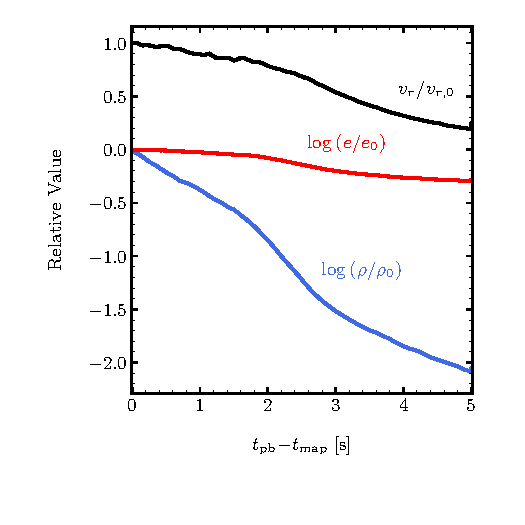
\includegraphics[width=0.50\textwidth,trim=0.2cm 1.1cm 0.2cm 0.2cm,clip]{./pic/wind_paper.pdf}
 \caption{Time-dependent behavior of neutrino-wind density $\rho$, radial velocity $v_{\mathrm{r}}$ and the total energy density $e$, normalized to their initial values at $t_{\mathrm{map}}\mathord{=}1.44\,\s$, which defines the start of the long-time simulation of model \znine. The data are extracted from a 1D simulation of the explosion of the $9.6\,\solm$ progenitor with \vertexprom (see \citealt{Mirizzi2016}), evaluated at a radius of 600 km. }
\end{figure}% END FIGURE WIND


\section{Evolution during the first second}
\label{sec:Evolution during the first second}
\subsection{Shock propagation, energetics and neutron star properties}
In the following we provide a short overview of the post-bounce phase. The reader is referred to \cite{Melson2015a} and \cite{Melson2019} for a detailed analysis of the post-bounce phase of the iron core progenitors. Generic features of the explosion of ECSNe are given in \cite{Kitaura2006,Janka2008,Gessner2018}. Since our results closely resemble these previous findings, we \GEO{summarize} the most important features in the following.
In Figure~\ref{fig:eexp all} we show the evolution of the angle-averaged supernova shock and the diagnostic explosion energy of our three-dimensional simulations during the post-bounce phase. 
The angle-averaged supernova shock is calculated as
\begin{equation}
    \langle R_{\mathrm{sh}} \rangle =  \frac{1}{4\pi}\int R_{\mathrm{sh}}(\theta,\phi)\ud \Omega,
    \label{equ:avg rsh}
\end{equation}
where $\ud \Omega\mathord{=}\sin{\theta}\ud\theta\ud\phi$.
The diagnostic explosion energy at any time is given by an integral of total (i.e. kinetic plus internal plus gravitational) specific post-shock binding energy, defined as $e_{\text{b}} = e_{\mathrm{int}} + e_{\mathrm{kin}} + \Phi_{\text{g}}$, over volume elements where it has a positive value 
\begin{equation}
    \mathrm{E}_{\mathrm{exp}} = \int_{M} e_{\mathrm{b}} \, \mathrm{dm'},\quad e_{\mathrm{b}} > 0.
    \label{equ:ene exp}
\end{equation}

The sharp drop in density outside the ONeMg-core of model \onemg leads to an early and strong drop in the accretion rate and hence ram pressure at the shock.
Consequently, the forward shock expands rapidly and reaches the core/envelope boundary ($R_{\mathrm{He/H}}\,\mathord{=}\,1210\,\text{km}$), at $0.18\,\s$ after core bounce.
This is in sharp contrast to the typical core-collapse supernova, where the high ram pressure stalls the shock expansion significantly for several $100\,\text{ms}$. The explosion energy starts rising steeply as soon as the forward shock leaves the ONeMg core.

\begin{figure*}
 \centering
 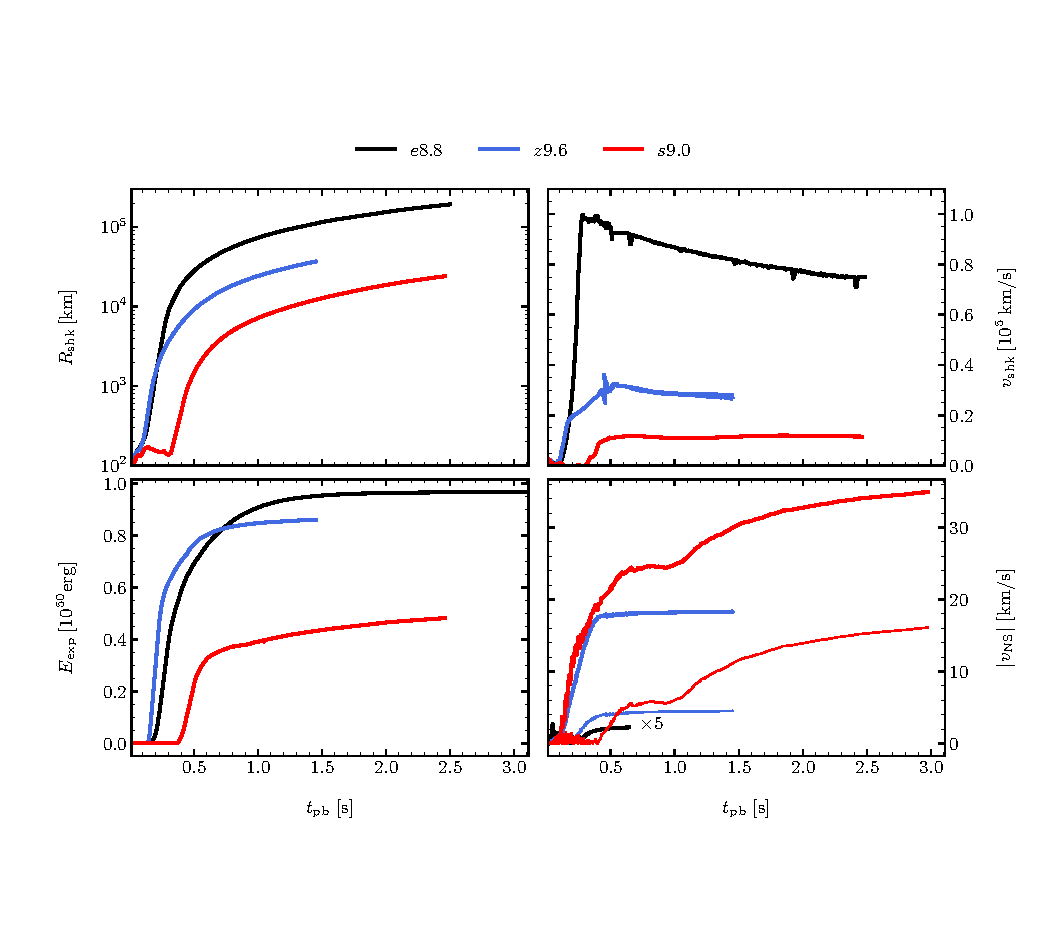
\includegraphics[width=\textwidth,trim=0.1cm 2.1cm 0cm 2.3cm,clip]{./pic/eexp_shk_kick_all_paper.pdf}
 \caption{Shock radius (upper left panel), shock velocity (upper right panel) and diagnostic explosion energy (lower left panel) versus post-bounce time for all of our 3D models. We also show the total PNS kick velocities (thick lines) and hydrodynamic induced PNS kick velocities (thin lines) in the lower right panel. \GEO{The difference is associated with the PNS kicks caused by asymmetric neutrino emission due to the LESA phenomenon (see text for details). For the iron core progenitors we can track only hydrodynamic contributions to the kick as soon as the transport module of \vertexprom is switched off, while for the ONeMg case our simplified neutrino treatment with the excised core of the PNS does not allow us to monitor the LESA induced kick.}The kick of model \onemg is scaled by a factor of 5 for better visibility. }
\label{fig:eexp all}
\end{figure*}

The acceleration of the shock at the core/envelope boundary is followed by a huge deceleration at the lower boundary of the H-envelope (see upper right panel of Figure~\ref{fig:eexp all}). This is caused by a sudden change of the density gradient at the core/envelope transition.  
Consequently, strong pressure waves are sent upstream into the ejecta, compressing and decelerating the neutrino-heated material.

\begin{table*}
\caption{Overview of PNS properties of our multi-dimensional models at $t_{\mathrm{map}}$.}
\label{tab:neutron star}
\begin{tabular}{cccccccccc||ccc}
    \hline 
            & $t_{\mathrm{map}}$ & 
            $v_{\mathrm{NS,tot}}$ & 
            $v_{\mathrm{NS}}^{\mathrm{hyd}}$ & 
            $v_{\mathrm{NS}}^{\nu}$ &
            $J_{\mathrm{NS}}$    & 
            $\alpha_{\mathrm{ej}}$&
            $\alpha_{\mathrm{ej}}^{\nu}$&
            $M_{\mathrm{b}}$ &
            \rns &
            $M_{\mathrm{fin}}$ &
            $M_{\mathrm{g}}$ &
            $P_{\mathrm{NS}}$ 
            \\
    Model &
    [s]   &
    [km/s] &
    [km/s] &
    [km/s] &
    $[10^{45}\, \mathrm{cm^2 g/s}]$ &
    [\%]              &  
    [\%]              &  
    [\solm]        &
    [km] &
    [\solm]         &
    [\solm]    &
    [s]     \\
    
    \hline
    % model                    tmap    vtot    vhy   vneut      Jns    alhy   alnu    mns        rns      mfin     mfing    pns   
    $e8.8_{3}^{\mathrm{2D}}$ & 2.515 & 1.55  & 1.55  & -     & 1.80  & 1.154 &  -     & 1.323 &  49.85 &  1.334 &  1.216 &  0.65 \\
    $e8.8_{6}^{\mathrm{2D}}$ & 2.515 & 0.94  & 0.94  & -     & 2.70  & 0.041 &  -     & 1.316 &  50.22 &  1.327 &  1.210 &  0.43 \\
    $e8.8_{10}^{\mathrm{2D}}$& 2.515 & 0.13  & 0.13  & -     & 4.19  & 0.004 &  -     & 1.308 &  50.57 &  1.319 &  1.203 &  0.27 \\
    $e8.8_{15}^{\mathrm{2D}}$& 2.515 & 0.59  & 0.59  & -     & 1.66  & 0.011 &  -     & 1.299 &  50.86 &  1.309 &  1.195 &  0.69 \\
    $e8.8_{10}^{\mathrm{3D}}$& 0.470 & 0.44  & 0.44  & -     & 0.69  & 0.004 &  -     & 1.307 &  50.57 &  1.326 &  1.209 &  1.68  \\
    \znine                   & 3.140 & 19.28 & 10.16 & 24.89 & 1.73  & 4.623 & 1.354  & 1.340 &  20.98 &  1.340 &  1.221 &  0.68 \\
    \snine                   & 1.440 & 36.32 & 29.65 & 26.22 & 7.60  & 10.02 & 1.178  & 1.299 &  19.58 &  1.299 &  1.128 &  0.15  \\
    \hline
\end{tabular}
\flushleft
\textit{Notes}: \GEO{All values are given at the end of our explosion simulation ($t_{\mathrm{map}}$). $v_{\mathrm{NS}}^{\mathrm{tot}}$ is the total NS kick resulting from the hydrodynamic ($v_{\mathrm{NS}}^{\mathrm{hyd}}$) plus the neutrino-induced ($v_{\mathrm{NS}}^{\mathrm{\nu}}$) contribution. $J_{\mathrm{NS}}$ is the total angular momentum transported to the PNS through a radius of 100 km \COM{I include inward and outward flux of angular-momentum}. $\alpha_{\mathrm{ej}}$ and $\alpha_{\mathrm{ej}}^{\nu}$ are the hydrodynamic and neutrino anisotropy-parameter, respectively (see Appendix~\ref{Appendix:Neutron Star Properties}). For the iron core progenitors we average $\alpha_{\mathrm{ej}}^{\nu}$ over the time the emission dipole is the largest until the end of the simulation. $M_{\mathrm{b}}$ is the baryonic PNS mass. $P_{\mathrm{NS}}$ is the PNS spin period at the end of our post-bounce simulations assuming a final PNS radius $R_{\mathrm{NS}}$ of 12 km, angular momentum conservation and a gravitational mass of $M_{\mathrm{g}}$. $M_{\mathrm{fin}}$ (see also Table~\ref{tab:long term boundaries}) is the mass contained within the excised region from which we calculate and gravitational mass $M_{\mathrm{g}}$ of the PNS. }
\end{table*}

%z9.6
The ECSNe-like structure of model \znine is reflected in the evolution of the forward shock and growth of the diagnostic explosion energy. Shock radii remain almost perfectly spherical \GEO{in both the \onemg and \znine}. Acceleration of the forward shock outside the iron core, however, is weaker in the \znine model than in model \onemg, due to the more gradual change in the density profile. Explosion energies also start to rise early and saturate just after $\tpb\mathord{\sim}1\,\s$.

%s9.0
In contrast to the \znine and \onemg models, the \snine is lacking the very steep density gradient outside the Fe-core, as can be seen in Figure~\ref{fig:prog_tem_rho_ye_rhor}
The shock can expand initially up to $180\,\km$ at $\tpb\mathord{\sim}130\,\ms$ but then \GEO{enters a phase of recession}. The \GEO{arrival} of the Si/O interface at the shock and \GEO{the decreasing mass-accretion rate} within the oxygen shell, eventually lead to shock expansion at $\mathord{\sim}0.3\,\s$ after bounce. Shock expansion is aided by strong convection behind the shock front. Similar to the results presented in \cite{Glas2019}, who used the same progenitor, the model remains convection-dominated and does not indicate any signs of the standing-accretion shock instability (SASI) \citep{Blondin2003,Foglizzo2007}.
However, although SASI does not develop in the simulation, the forward shock experiences \GEO{large-scale deformations with a dipole amplitude of $10\mathord{-}10\%$ (compared to the angle-averaged shock radius)}. These deformations are driven by large scale plumes that form in the post-shock layer. 
Contrary to the ECSN-like models, strong non-radial motions persist \GEO{around the PNS} over several seconds after bounce. Continuous mass accretion on the PNS through small funnels delay the emergence of the spherical neutrino-driven wind, which is why we needed to continue the simulations over three seconds after bounce.

%% FIGURE Initial Ni+X all Progenitors
\begin{figure*}
 \centering
 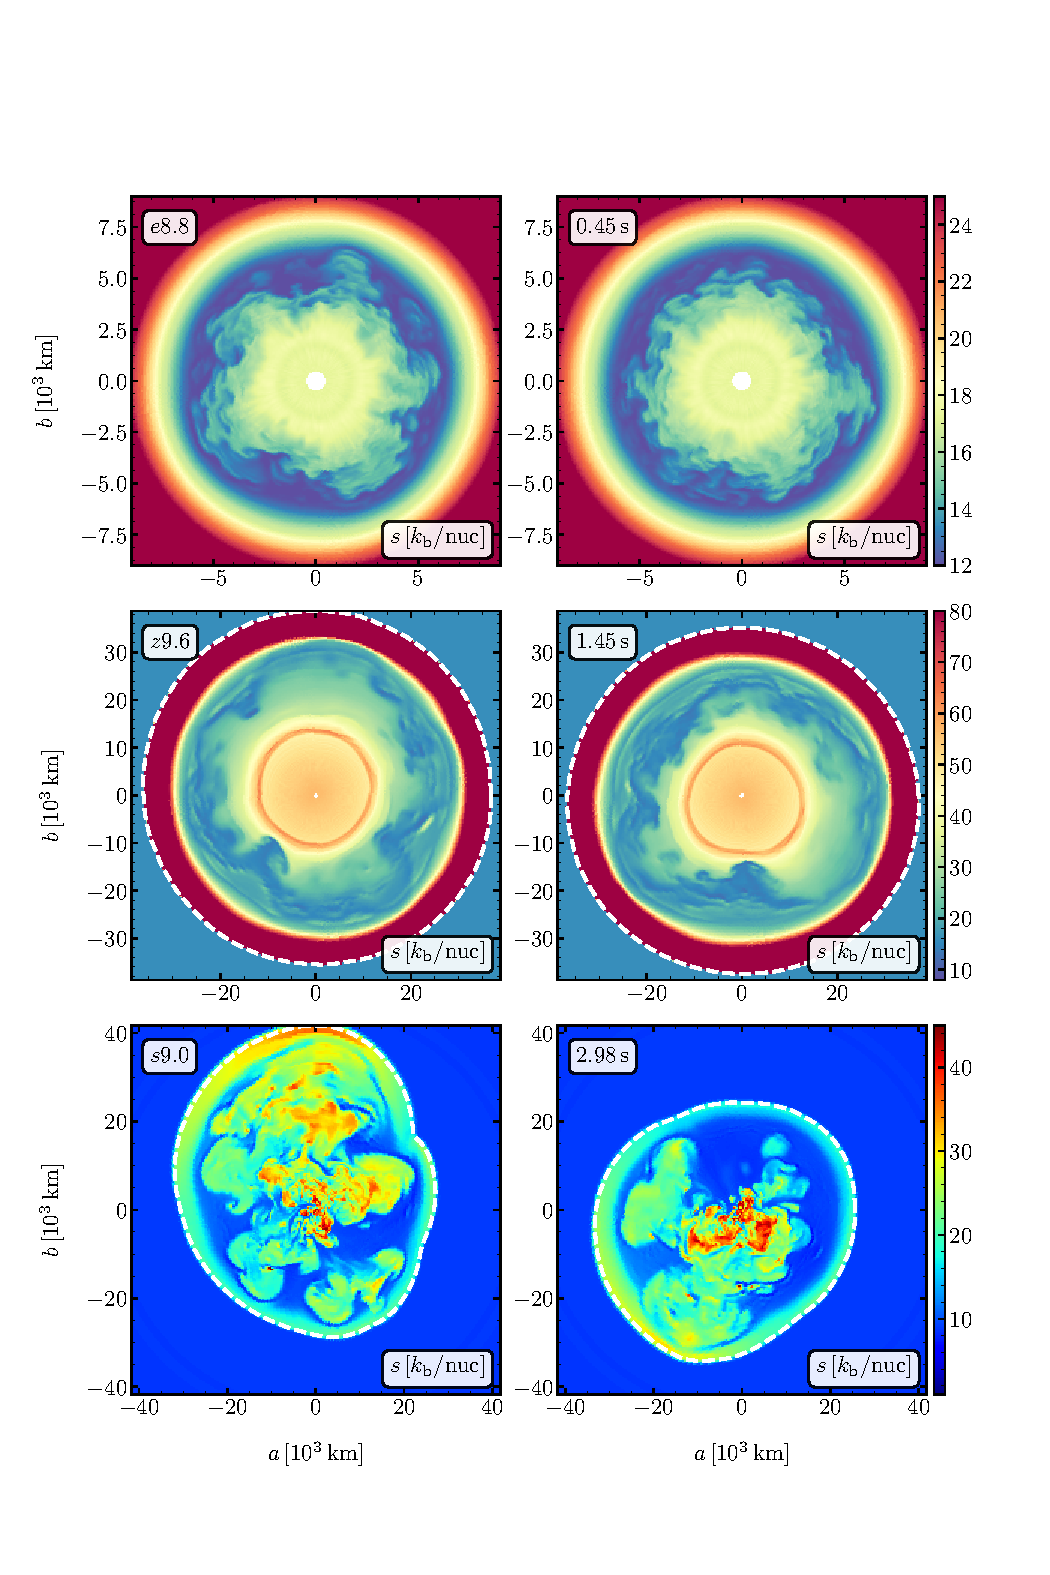
\includegraphics[width=0.95\textwidth,trim=0cm 1.8cm 0cm 3cm,clip]{pic/all_3d_sto_slices_time_0.pdf}
 \caption{Planar cuts of our 3D models showing the entropy color-coded at $t_{\mathrm{map}}$. The left panels display cuts which are aligned such that the point of largest shock deformation is included in the plane. Therefore the coordinate directions of the plots have no association with the computational-grid coordinates. The right panels include the smallest shock expansion in the plane. Note the largely spherical morphology of model \onemg and the deformed ejecta morphology of model \snine. For better visibility of the small scale structures of model \snine we chose a different color representation in this case.}
 \label{fig:slices first mapping}
\end{figure*}
In order to compare the final state of the post-bounce simulations of our model set, we \GEO{present} in Figure~\ref{fig:slices first mapping} planar cuts showing the entropy at the times ($t_{\mathrm{map}}$) we start our long-time simulation. The left panels are chosen such that they include the plane of the largest shock deformation. The right panels include the plane of the smallest shock deformation.
Note the \GEO{basically spherical shape of the shock and the mild post-shock asymmetries} in both the \onemg and \znine models.
In strong contrast to the ECSNe-like models, the \snine shows a clear dipolar shock deformation and ejecta morphology. 

The asymmetries that develop during the explosion also affect the kick of the PNS.
In Table~\ref{tab:neutron star} we provide properties of the PNS resulting from our post-bounce simulations\footnote{We refer the reader to Appendix~\ref{Appendix:Neutron Star Properties} for the equations involved in the analysis presented in Table~\ref{tab:neutron star}.}. We list the PNS kick velocity ($v_{\mathrm{NS}}$), anisotropy parameter ($\alpha_{\mathrm{ej}}$), angular momentum ($J_{\mathrm{NS}}$) and spin period ($P_{\mathrm{NS}}$) along with the PNS radii (\rns) and baryonic PNS masses ($M_{\mathrm{b}}$) at the point in time we terminate the post-bounce simulations. The PNS radius $\rns$ is defined as the angle-dependent radius where the density drops below $10^{11}\,\mathrm{g/cm^3}$. The PNS mass $M_{\mathrm{b}}$ is the mass contained within $\rns$. $M_{\mathrm{fin}}$ is the mass contained within our inner boundary for the long-time simulations (see Table~\ref{tab:long term boundaries}) and $M_{\mathrm{g}}$ the respective gravitational mass.
The acceleration of the PNS is caused by two different mechanisms.
\GEO{Firstly, aspherical ejection of matter leads to a gravitational ``tug'' which accelerates the PNS in the opposite hemisphere of maximum shock expansion and fastest ejecta. Second, anisotropic neutrino emission, due to the ``lepton-emission self-sustained asymmetry'' (LESA) \citep{Tamborra2014}, can accelerate the PNS opposite to the direction of the largest total neutrino-energy flux.
The almost spherical explosions of the ECSNe-like progenitors yield low hydrodynamic kick velocities. Anisotropic neutrino emission does not play a role in the simulation of model \onemg, because of the spherical treatment of the central region. The contribution of anisotropic neutrino emission in models \znine and \snine, however, even exceeds the contribution due to aspherical ejection of matter. LESA manifests itself in a dominant and stable $\ell\mathord{=}1$ mode of the lepton-number emission and a corresponding energy-emission dipole of several percent amplitude compared to the monopole (see \citealt{Tamborra2014}). LESA is observed in both simulations conducted with \vertexprom. }

We show in Figure~\ref{fig:sto ye s9 z9 kick} planar slices of the electron fraction (left panels) and entropy (right panels) of the iron core progenitors. The black, blue and green arrows indicate the total, hydrodynamic and neutrino-induced directions of the PNS kick. In case of the \znine the hydrodynamic and neutrino-induced kicks are clearly aligned. This stems from the feedback mechanism which is associated with LESA. Increased heating in the direction opposite to the LESA dipole pushes the supernova shock to larger radii. The induced asymmetry of the post-shock ejecta feeds back into the hydrodynamic acceleration of the PNS. Due to the weak convection in the \znine model, the emission asymmetry is the dominant contribution to drive the PNS kick. 
Where the gravitational tug can only account for  $v_{\mathrm{NS}}^{\mathrm{hyd}}\mathord{\sim}10\,\kms$, the asymmetric emission of neutrinos enables a kick velocity up to $v_{\mathrm{NS}}^{\mathrm{\nu}}\mathord{\sim}25\,\kms$. The total kick sums up to $v_{\mathrm{NS}}^{\mathrm{tot}}\mathord{=}19\,\kms$.
The alignment of the neutrino-induced and hydrodynamic kick is less clear in model \snine. Although the neutrino emission is the largest contribution to the total PNS kick during the first 500 ms, strong non-radial motions in the post-shock region interfere with the LESA feedback mechanism and thus the LESA induced kick. 
The hydrodynamically induced dipolar shock expansion of model \snine and contributions from the LESA dipole yield a total acceleration of the PNS to $v_{\mathrm{NS}}\mathrm{\sim}36.32\,\kms$.
\COM{Question: What effect has the early disabling of neutrino transport? Neutrino-induced kick has not saturated. }

\begin{figure*}
 \centering
 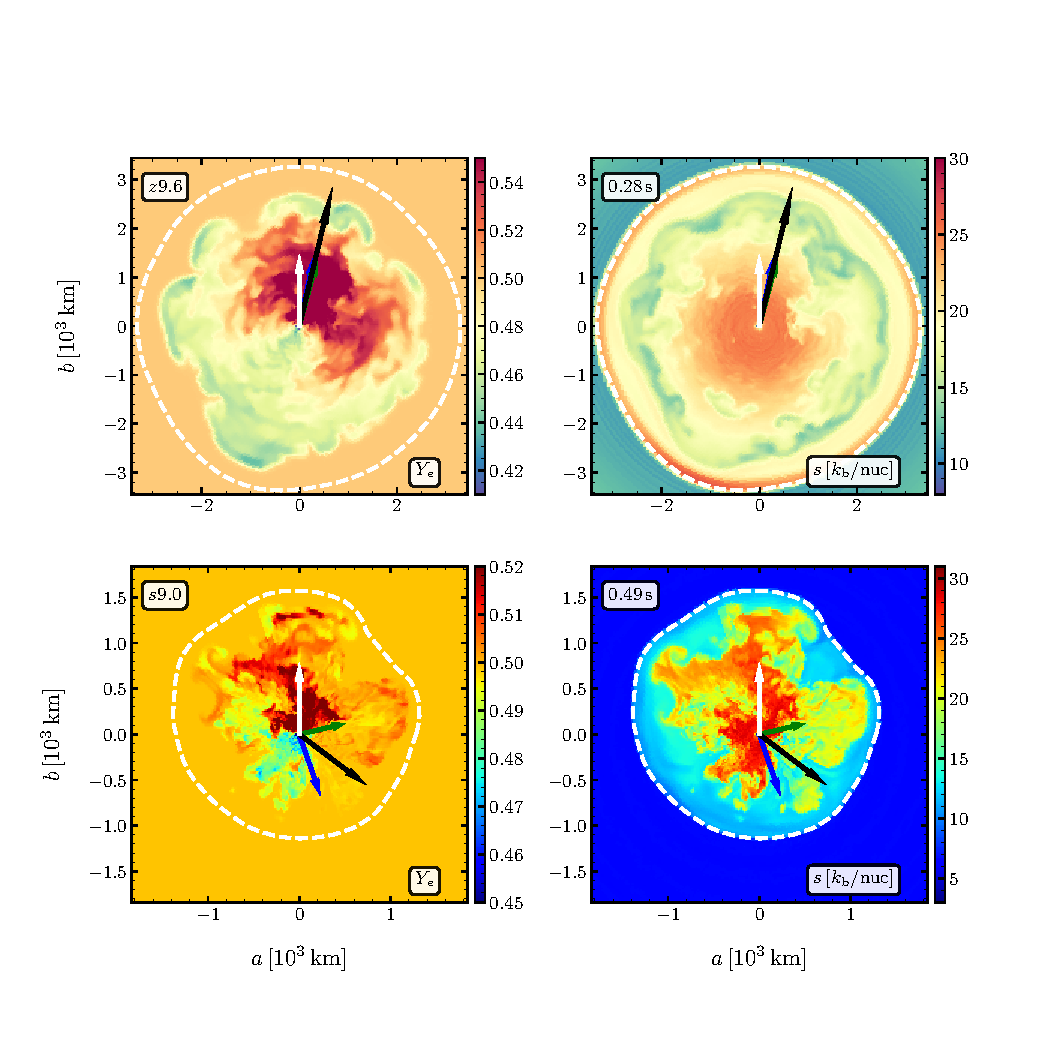
\includegraphics[width=\textwidth,trim=0cm 1.3cm 0cm 2cm,clip]{pic/z9_s9_3d_ye_sto_kick_slices_paper.pdf}
 \caption{\GEO{Planar slices of the electron fraction $Y_{e}$ (left panels) and entropy (right panels) of models \znine and \snine. The planes are chosen such that the LESA dipole direction (white arrow) is pointing to the north and are not aligned with the global coordinate system. The arrows indicate the direction of the total kick (black), the hydrodynamic and neutrino kick (blue and green).}}
 \label{fig:sto ye s9 z9 kick}
\end{figure*}

\subsection{Extent of mixing at shock revival}
\label{sec:Extent of mixing at shock revival}

In order to access the strength of mixing during the first second in our 3D models, we present in Figure~\ref{fig:mdp first mapping} fractions of the total mass of selected elements as a function of velocity (top panels) and mass coordinate (lower panels). 
For sampling the velocity space, we chose 50 bins between the maximal and minimal velocities within the considered region. We use 30 bins to sample the distribution in mass coordinate.

The spherical explosion of the \onemg manifests itself also in the distribution of elements over mass and velocity space, where the initial shell-like structure of the progenitor is maintained.
The thin carbon-shell of the progenitor is traveling with $\sim 40\mathord{-}50\,\mathrm{1000\,km/s}$ in front of the outer mass-shells of the former ONeMg-core, which travel at $\sim 35\,\mathrm{1000\,km/s}$. Most of the newly synthesized iron-group and $\alpha$ nuclei travel at velocities below $\sim 35\,\mathrm{1000\,km/s}$.
Early deceleration of the shock also confines the neutrino-heated ejecta within $M(r)\mathord{\le 1.33}\,\solm$.

%z9.6
Slightly more violent convection in the \znine model lead to more efficient mixing in mass and velocity space (see left panels of Figure~\ref{fig:mdp first mapping}). Some neutrino-heated material could already be mixed into the carbon and oxygen shells that travels at $20\times 10^3\,\kms$. The bulk of the metal-rich ejecta still travels with slower velocities, however. 
Similar to the \onemg, the deceleration of the forward shock at the Si/O and CO/He interfaces in the \znine also compressed some of the matter into a dense shell. 
%s9.0 
The \snine model, again, differs strongly from the ECSN-like models. 
Long-lasting convection completely erased the initial onion-like shell structure of the progenitor. Elements are homogenously mixed over mass and velocity coordinate (see middle panels of Figure~\ref{fig:mdp first mapping}).
The fastest neutrino-heated ejecta are caused by a large high entropy plume inducing a bipolar perturbation on the shockwave, which can be see in Figure~\ref{fig:slices first mapping}.

%% FIGURE Mass Distribution all Progenitors
\begin{figure*}
 \centering
 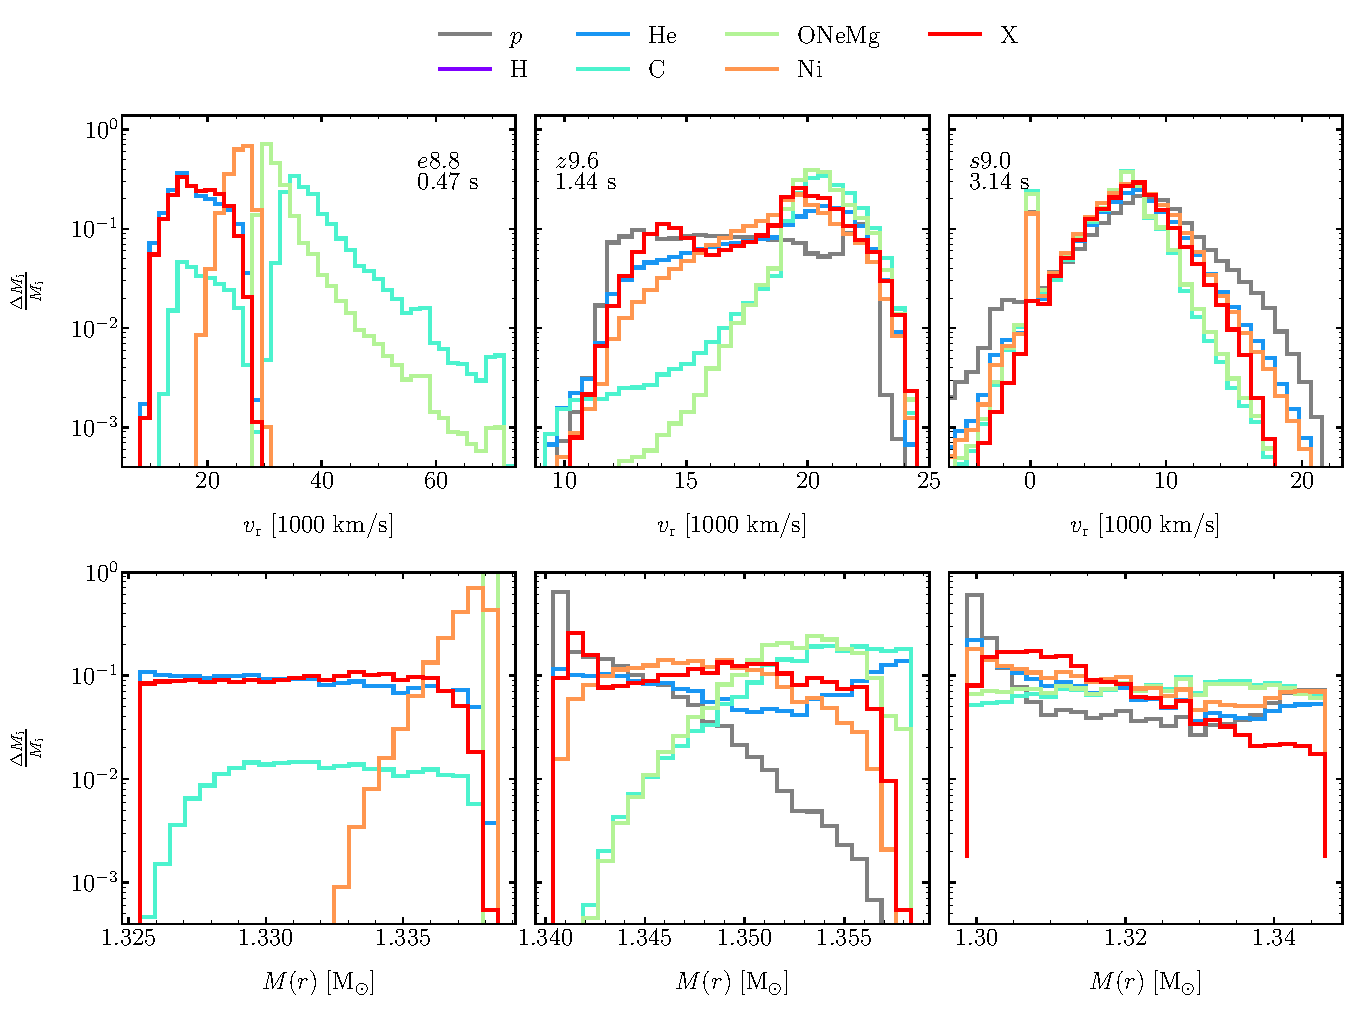
\includegraphics[width=\textwidth,trim=0.0cm 0.0cm 0cm 0cm,clip]{pic/z96_s9_e8_3d_massDis_mvr_and_masstime_0_paper.pdf}
 \caption{Binned distribution of elements as a function of radial velocity (top panels) and enclosed mass (bottom panels) for all our 3D models at $t_{\mathrm{map}}$ (see Table~\ref{tab:long term boundaries}). We use 50 bins in velocity space and 30 bins in mass coordinate. See text for discussion.}
 \label{fig:mdp first mapping}
\end{figure*}
\iffalse
\begin{table*}
    \centering
    \begin{tabular}{lcc}
        &
        \multicolumn{2}{c}{\onemg} \\
         Species &
         $M_{\mathrm{init}}$ &
         $M_{\mathrm{fin}}$ \\
                 &
         $[M_{\mathrm{\odot}}]$ &
         $[M_{\mathrm{\odot}}]$ \\
         \hline 
            p               & 2.7                & 2.895e+00 \\
            He4             & 1.8                & 1.745e+00 \\
            C12             & $2.2\times10^{-2}$ & 2.196e-02 \\
            O16+Ne20+Mg24   & $5.0\times10^{-2}$ & 4.972e-02 \\
            Ni56+Fe56       & $3.4\times10^{-3}$ & 2.653e-03 \\
            X56             & $1.3\times10^{-2}$ & 1.301e-02 \\
            rest            & $5.6\times10^{-2}$ & 5.593e-02 \\
            \hline \\
            X Sum           & 4.641e+00 & 4.583e+00 \\
            + pm            & 5.959e+00 & 5.901e+00   
    \end{tabular}
    \caption{Caption}
    \label{tab:my_label}
\end{table*}
\fi

\section{Evolution until Shock-Breakout}
\label{sec:Evolution until Shock-Breakout}
\subsection{Linear stability analysis}
\label{sec:Linear stability analysis}
As already mentioned, the velocity of the forward shock depends on the progenitor structure, in particular the $\rho r^3$-profile. According to \cite{Sedov1961} one expects a \GEO{increase/decrease} in the shock velocity when the gradient of the $\rho r^3$-profile is positive/negative. 
\GEO{This acceleration and deceleration leads to crossing of the density and pressure gradients in the post-shock region, or stated otherwise, the gradients of the pressure and density have opposite signs.} Thus, perturbations in the matter become unstable to the Rayleigh-Taylor instability \citep{Rayleigh1882,Chevalier1978}. As the $\rho r^3 $-profiles, and hence the shock speed, vary significantly between the progenitors, growth of Rayleigh-Taylor instabilities will affect the long-time evolution of our models in different ways.

In order to aid us with the interpretation of our three-dimensional simulations, we appeal to 1D simulations which are started from angle-averaged initial states of the 3D data. The numerical and physical setup for the spherically symmetric simulations remains unchanged. 
They can teach us about the behavior of the shock, while it propagates through the envelope. 
Additionally, we compute the linear RT growth rates $\sigma_{\mathrm{RT}}$ of small initial perturbations by tracking Lagrangian mass coordinates in our 1D simulations, following \cite{Mueller1991}. 
In the incompressible case the growth rate is given by
\begin{equation}
  \label{equ:growth rates incmp}
  \sigma_{\mathrm{RT,incmp}} = \sqrt{- \frac{p}{\rho}\frac{\partial \ln p}{\partial r}\frac{\partial \ln \rho}{\partial r}},
\end{equation}
where $p$ and $\rho$ are the pressure and density. In the compressible case the growth rate becomes
\begin{equation}
  \sigma_{\mathrm{RT, cmp}} = \frac{c_{s}}{\gamma}\sqrt{\Big(\frac{\ln p}{\partial r}\Big)^ 2 - \gamma \frac{\partial \ln p}{\partial r}\frac{\partial \ln \rho}{\partial r}},
  \label{equ:growth rates cmp}
\end{equation}
where $c_{\mathrm{s}}$ is the speed of sound and $\gamma$ the adiabatic index. Equation~\ref{equ:growth rates cmp} is less restrictive than its incompressible counterpart\footnote{Note that we are interested in the locations of maximal growth but not in the actual values. Calculating the growth factors from multidimensional models using angle averaged values gives similar overall structure but lower amplitudes \citep{Mueller2018}.}. 
For the time-dependent amplification factor we integrate Equation~\ref{equ:growth rates cmp} according to
\begin{equation}
  \Sigma_{\rm RT}(t) = \frac{\xi}{\xi_0}(t) = \exp \left(\int_0^t \sigma_{RT} (t') dt' \right).\label{equ:growth rates int}
\end{equation}
This analysis enables us to estimate the time and locations in mass coordinate, where the fluid becomes unstable to the RTi and thus helps us to understand the origin of outward/inward mixing of \GEO{different layers with their chemical elements}.

We show in Figure~\ref{fig:growth rates} the amplification factors in the incompressible (colored lines) and compressible (gray line) cases for our spherically symmetric simulations. Significant differences between the models are evident.
\begin{figure*}
 \centering
 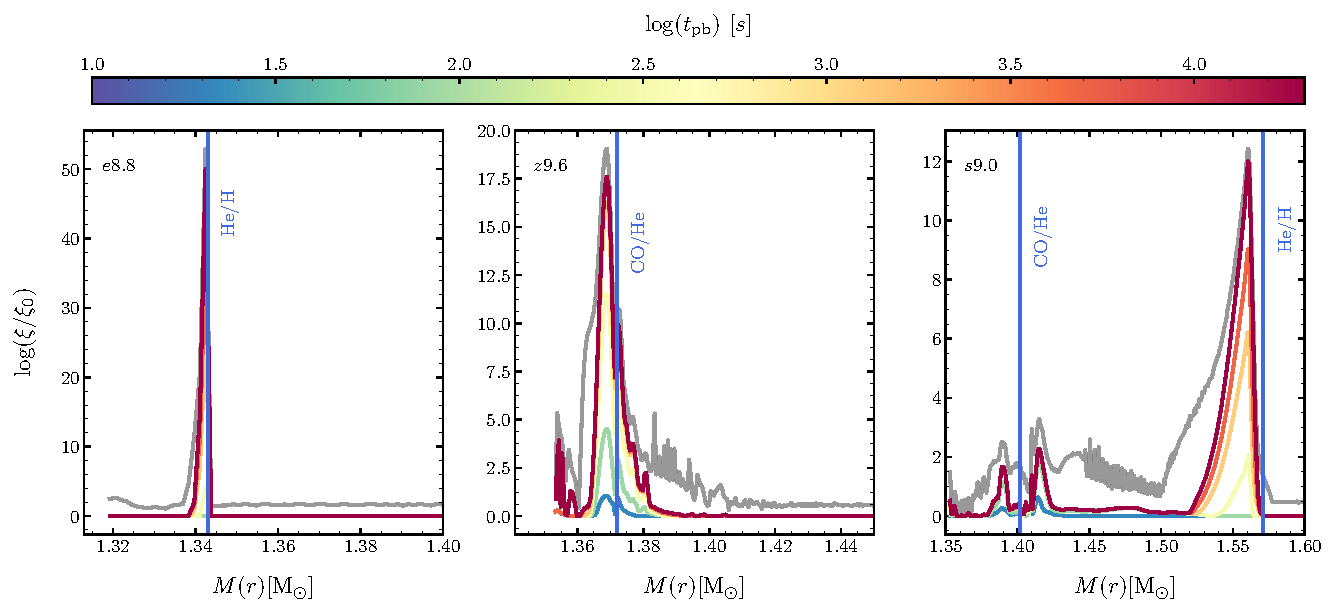
\includegraphics[width=\textwidth]{pic/growth_rates_1d_paper.pdf}
 \caption{Integrated growth rates for all considered models at different times evaluated with Equation~\ref{equ:growth rates int} (colored lines). Indicated by the blue lines are the respective composition interfaces. The gray line denotes the evaluation of the growth rates in the compressible case at $t=10^{4}\,\text{s}$. The different progenitor structures have a large impact on the estimated growth as can be seen most prominently by comparing mode z9.6 and s9.0. Where the ECSNe-like progenitors develop only a small region of instability around the interface with the steepest density gradient (e.g. He/H for model \onemg and CO/He for model \znine), model \snine shows three distinct peaks of the growth factor at the Si/CO, CO/He and the He/H interfaces. }
 \label{fig:growth rates}
\end{figure*}

The left panel of Figure~\ref{fig:growth rates} shows the integrated growth-rate of the $e8.8_{10}$ model.
The extreme deceleration of the forward shock when moving into the hydrogen envelope induces very high growth factors at $M(r)\mathord{\sim}1.34\,\mathrm{M_{\odot}}$.
The ECSN-like structure of model \znine is reflected in the amplification factors.
Strong deceleration of the forward shock at the core/hydrogen interface created the necessary condition for the RTi to grow. As can be seen in Figure~\ref{fig:growth rates}, amplification factors at $\mathord{\sim}1.36\,\solm$ between the C/He and He/H interfaces of model \znine (see Table~\ref{tab:progenitors}) almost reach values as high as observed in the ECSN case. Interestingly, no growth is expected at the He/H interface, which stems from the very small step in the $\rho r^3$ profile at this interface (see Figure~\ref{fig:prog_tem_rho_ye_rhor}).
Model \snine shows striking differences to the models described above. 
Due to its more shallow $\rho r^3$-profile in the core region and the consequently weaker episodes of de- and acceleration, the peak amplitudes of the growth factors are smaller. They are, however, of the same strength as in the more massive models investigated by \cite{Wongwathanarat2015}. 
\GEO{
Three distinct regions of instability can be discerned at the Si/CO, CO/He and He/H interfaces. 
Similar to the red supergiants presented in \citet{Wongwathanarat2015}, the strongest contribution arises from the He/H interface followed by the CO/He interface where amplification factors  reach values of $5-10$, respectively. 
While the compressible and incompressible analysis gives similar results for models \onemg and \znine, the compressible evaluation of the growth factors in model \snine predicts additional growth within the He-core of the star. This is caused by the passage of the reverse shock at later times ($\tpb\mathord{>}3\mathord{\times}10^3\,\s$). Note that, at this stage, the instability is already in a strongly non-linear phase, where Equation~\ref{equ:growth rates cmp} losses its validity.
}
%% NEW STUFF
\subsection{Propagation of the forward shock}

We show in Figure~\ref{fig:radii all times} the angle-averaged shock radii $R_{\mathrm{sh}}$, reverse shock radii $R_{\mathrm{rsh}}$ and shock velocities $v_{\mathrm{sh}}$ of our 3D long-time simulations.
The forward shock of model \onemg has long passed the He/H interface and is traveling through the H-envelope.
It left the core with some $75,000\,\kms$ and is progressively decelerated 
due to the monotonically increasing $\rho r^3$ within the H-envelope. 
Since the innermost neutrino-heated ejecta are not in sonic contact with the 
supernova shock, they do not feeld the deceleration and thus travel with constant velocity of $\mathord{\approx}3,000\,\kms$ until they catch up with the immediate post-shock matter $\tpb\mathord{\approx}130\,\s$.
The interaction of the dense neutrino-heated ejecta with the post-shock material pushes the shock to higher velocities (see Figure~\ref{fig:radii all times}).
Thereafter, the forward shock decelerates continuously (without any phases
of acceleration) until it reaches the surface of the star. Note the large deceleration of the shock from its 
initial very large velocities of $75,000\,\kms$
down to $\mathord{<}1000\,\kms$ as it leaves the star. Most of the kinetic energy of the shockwave is used in
heating the hydrogen in the outer layers of the envelope.

The early strong deceleration of the forward shock at the edge of the core at $\tpb\mathord{=}0.19\,\text{s}$ has
lead to the compression of the CO and He layer into a high density shell. Less than $1\,\s$ later, a strong
reverse shock forms at its inside as the forward shock is progressively slowed down.
The dense shell separates the post shock material from the innermost ejecta as can be seen
in the density profile shown in Figure~\ref{fig:density profiles all times}. The formation of the dense shell or ``wall'' 
\cite{Kifonidis2006} has important consequences for the evolution of the metal-rich ejecta as well as for the growth
of Rayleigh-Taylor instabilities.

After $\tpb\mathord{\approx}\,1\text{h}$, continuous deceleration of the forward
shock causes the reverse shock to travel back in mass coordinate.
(see Figure~\ref{fig:density profiles all times}). It takes, however, approximately
$7\,\text{h}$ for the reverse shock to reach the inner boundary of our computational domain. 

% z9.6 1D
The forward shock of model \znine has already crossed the CO/He interface at $t_{\mathrm{map}}$
and is traveling at roughly $27,000\,\kms$. 
Behind the shock, a dense shell has formed due to the deceleration
and acceleration at the CO/He interface.
Above the interface and similar to model \onemg, 
a featureless density profile in the He-core and hydrogen envelope leads to an 
untroubled expansion of the forward shock which reaches 
the stellar surface at around $\tpb\mathord{\approx}\,1.12\,\mathrm{d})$. 
At the time of shock breakout the forward shock only travels at $<1000\,\kms$ due to
the large deceleration in the hydrogen envelope of the star. 
Different to the ECSN progenitor the reverse shock forms within the He-core of the star
(see Figure~\ref{fig:density profiles all times}) but also fairly early at some $\tpb \mathord{\approx} 15\,\s$.

Within the next $1000\,\s$, the reverse shock propagates back in radius and reaches the inner boundary
at $\tpb \mathord{\approx} 1.14\,\text{h}$, which is more than 4 hours earlier than in model \onemg. 

% s9.0 1D
The trajectories of the forward and reverse shock in the 1D simulation of model \snine 
are shown in the bottom left panel of Figure~\ref{fig:radii all times}. 
The simulation is initiated at $\tpb\mathord{=}3.1\,\s$, when the forward shock has just crossed the CO/He interface
and is traveling at $v_{\mathrm{sh}}\mathord{\approx} 9,000\,\kms$, just a fraction of the shock
velocity found in the ECSNe-like models. De- and accelerations of the supernova shock at the Si/O and 
C/O interfaces caused the formation of dense shells in the 
post-shock region (see Figure~\ref{fig:density profiles all times}).
The density contrast between the shells and the ejecta is,
however, around one magnitude smaller than found for the dense shells which formed at the core/envelope
boundary in model \onemg and at the CO/He interface in model \znine. 
In the following, the shock slows down rapidly within the He-core of the star down to 
$v_{\mathrm{sh}}\mathord{\approx}10,000\,\kms$ before it accelerates again at the outer
boundary of the He-shell reaching almost its initial velocity (at $\tpb\mathord{=}200\,\s$).
This is due to 
the steep density gradient just below the He/H interface in the progenitor. 
Thereafter, the forward shock encounters the increasing $\rho r^3$ in the hydrogen envelope and is 
thereby strongly decelerated, causing a compression of the post-shock material into a dense shell. 
At the bottom of the shell a strong reverse shock forms shortly afterwards (see also the density profiles 
in Figure~\ref{fig:density profiles all times}). Note that the formation of the reverse shock transpires 
well after than observed in the ECSN-like progenitors. 
Eventually the reverse shock reaches the inner boundary of our numerical grid at 
$\tpb\mathord{\approx}25\,\mathrm{h}$. Shock breakout occurs at $\tpb\mathord{\approx}1.2\,\mathrm{d}$.


\begin{figure*}
 \centering
 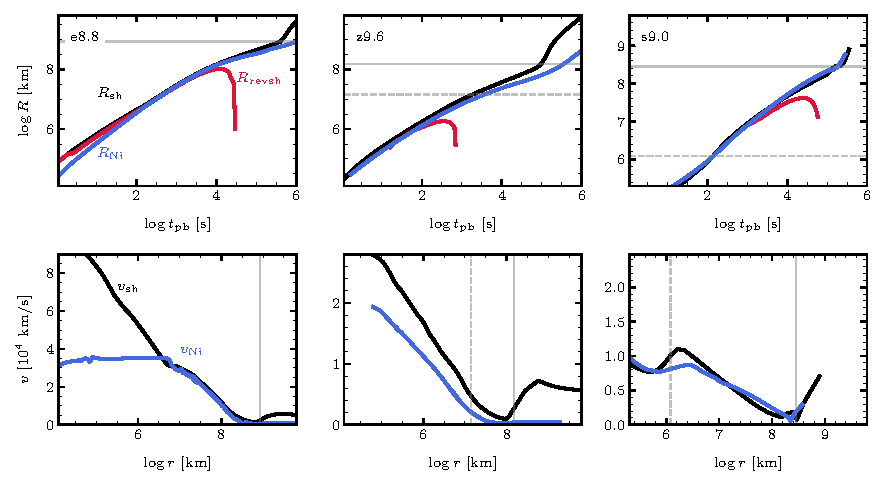
\includegraphics[width=\textwidth]{pic/radii_velocity_shock_nickel_paper.pdf}
 \caption{   
  \textit{Upper~panels}: Angle-averaged shock radius $R_{\mathrm{sh}}$ (black),
 angle-averaged reverse shock radius $R_{\mathrm{rsh}}$ (red) and maximum radius of the 
 $X_{\nickel\mathord{+}\tracer}\mathord{=}0.03$ iso-surface (blue). 
 \textit{Lower~panels}:
 Shock velocity $v_{\mathrm{sh}}$ (black) and velocity of the 
 $X_{\nickel\mathord{+}\tracer}\mathord{=}0.03$ iso-surface (blue) 
 of our 3D long-time simulations. 
 The expansion of the forward shock in the ECSNe-like progenitors proceeds without
 any phases of deceleration and acceleration. 
 In contrast, the forward shock in model \snine accelerates strongly before the He/H interface.
 The reverse shocks in models \onemg and \znine form within $\mathord{\approx}1\,\s$ and 
 $\mathord{\approx}10\,\s$, respectively, 
 whereas we observe the formation of a reverse shock in model \snine at
 $\mathord{\approx} 2,500\,\s$.
 Note that, in model \snine, the velocity of the $\nickel \mathord{+} \tracer$ 
 surface is higher than the average shock velocity within the hydrogen envelope of the star.
 }
 \label{fig:radii all times}
\end{figure*}

\begin{figure*}
 \centering
 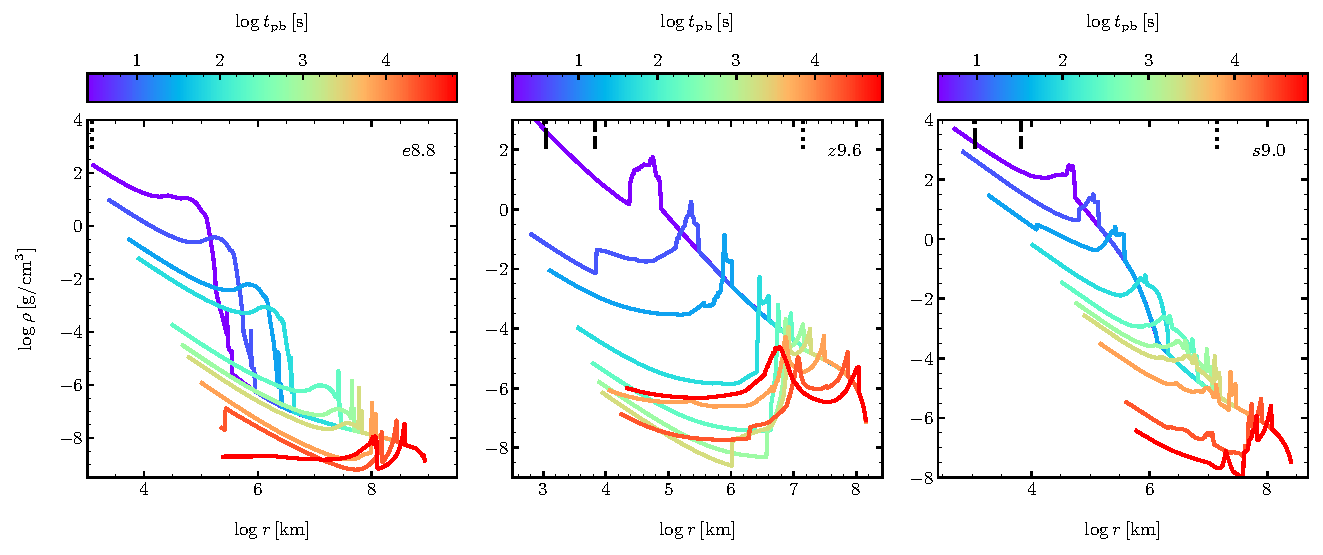
\includegraphics[width=\textwidth, trim=0cm 0.0cm 0cm 0.0cm,clip]{pic/density_profiles_1d_long_term.pdf}
 \caption{Radial profiles of the density of our 1D long-time simulations at representative times. The dashed, dash-dotted and dotted lines represent the outer boundaries of the iron-, CO and He cores. See text for discussion.}
 \label{fig:density profiles all times}
\end{figure*}

\subsection{Morphology of neutrino-heated ejecta}
In the following we focus on the long-time development of the early time asymmetries which we trace by the propagation of the neutrino-heated ejecta or more specifically the $\nickel\mathord{+}\tracer$-rich material. \cite{Kifonidis2003} already noted that \nickel is produced between the high-entropy bubbles that expand due to strong neutrino-heating from below. Thus the distribution of \nickel traces the asymmetries that developed during the onset of the explosion. 

% e8.8
In Figure~\ref{fig:e8 nix cuts} we show slices of the $\nickel\mathord{+}\tracer$ mass fraction of the 3D simulation of model \onemg. The dashed white line indicates the shock radius, whereas the thin dotted white line indicates the position of the mass shell of the He/H interface.

\begin{figure*}% Figure e8.8 NiX cuts
 \centering
 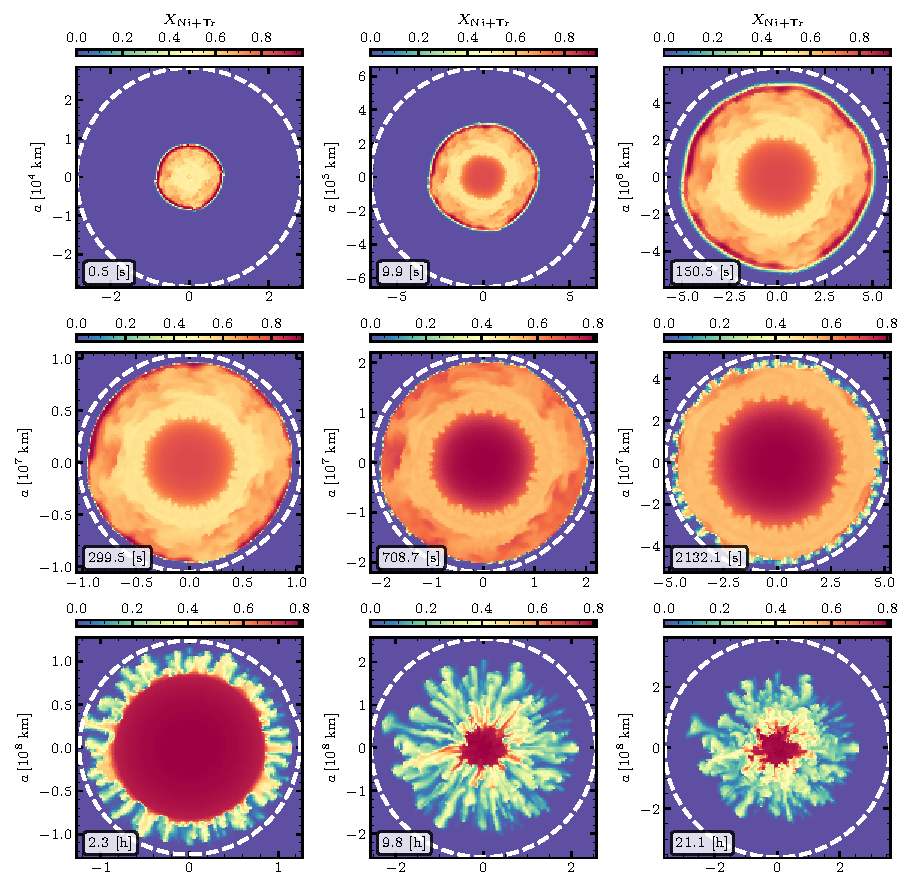
\includegraphics[width=\textwidth,trim=0.2cm 0cm 0cm 0cm,clip]{pic/e8_3d_3x3_NiX.pdf} 
 \caption{Slices
    showing the $\nickel\mathord{+}\tracer$ mass fraction in the 3D simulation of model \onemg. The dashed white curve indicates 
    the position of the supernova shock. Cyan colored regions represent the atmosphere of the progenitor. Until $\mathord{\approx}150\,\s$ the neutrino-heated 
    ejecta essentially expand self-similarly. This untroubled expansion stops at
    $300\,\s$, when the material is decelerated at the dense shell 
    (see Figure~\ref{fig:density profiles all times}). At $\mathord{\approx}2100\,\s$
    the growing RTI at the He/H interface clearly begin to affect the outer 
    layers of the neutrino-heated ejecta. Until $2.5\,\text{h}$ the plumes 
    grow in size, while the reverse shock (visible at the base of the plumes)
    begins propagate back in radius. $9.8\,\text{h}$ after bounce the reverse
    shock reaches the central object and compresses the metal
    rich ejecta. Note that the plumes are evenly distributed in angular direction and radial extent. }
 \label{fig:e8 nix cuts}
\end{figure*}

\begin{figure*}% --------------- FIGURE rho cuts 3d
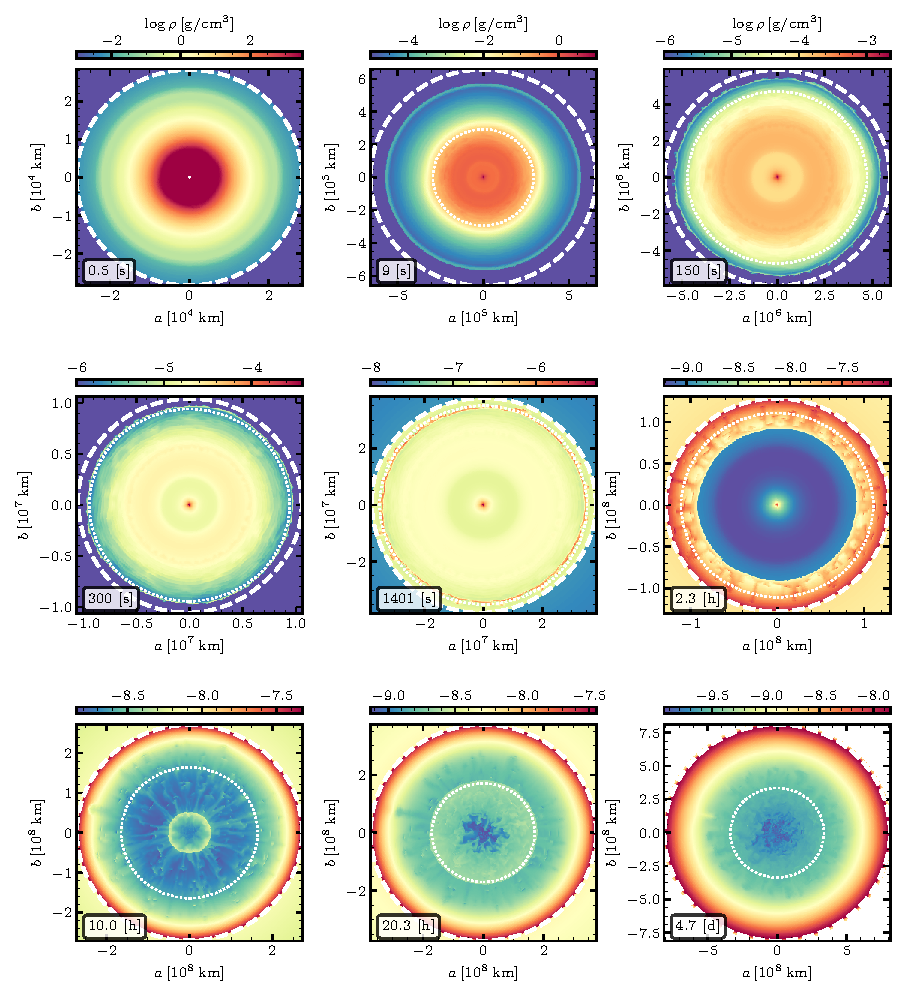
\includegraphics[width=\textwidth]{pic/e8_3d_3x3_den.pdf}
    \caption{Slices showing the density distribution
    in the 3D simulation of model \onemg. Cyan colored regions represent the atmosphere of the progenitor.  The dense shell at which the reverse shock 
    forms is visible as the light yellow ring with a radius of $\mathord{\approx} 2\mathord{\times}10^4\,\rm km$
    (see first panel).
    The panel at $\tpb\mathord{=}150\,\s$ show the formation of small RT fingers.
    These Fingers grow with time and affect the neutrino-heated material (see panel at
    $\tpb\mathord{\approx}1400 \, \s$).
    At $\tpb\mathord{\approx}3.4\,\rm d$ the innermost ejecta are characterized by an overall
    spherical shape, superimposed with the remains of the RT fingers.}
\label{fig:e8 rho cuts}
\end{figure*}% ---------------


\begin{figure*}% --------------- FIGURE e8.8 3d rendering
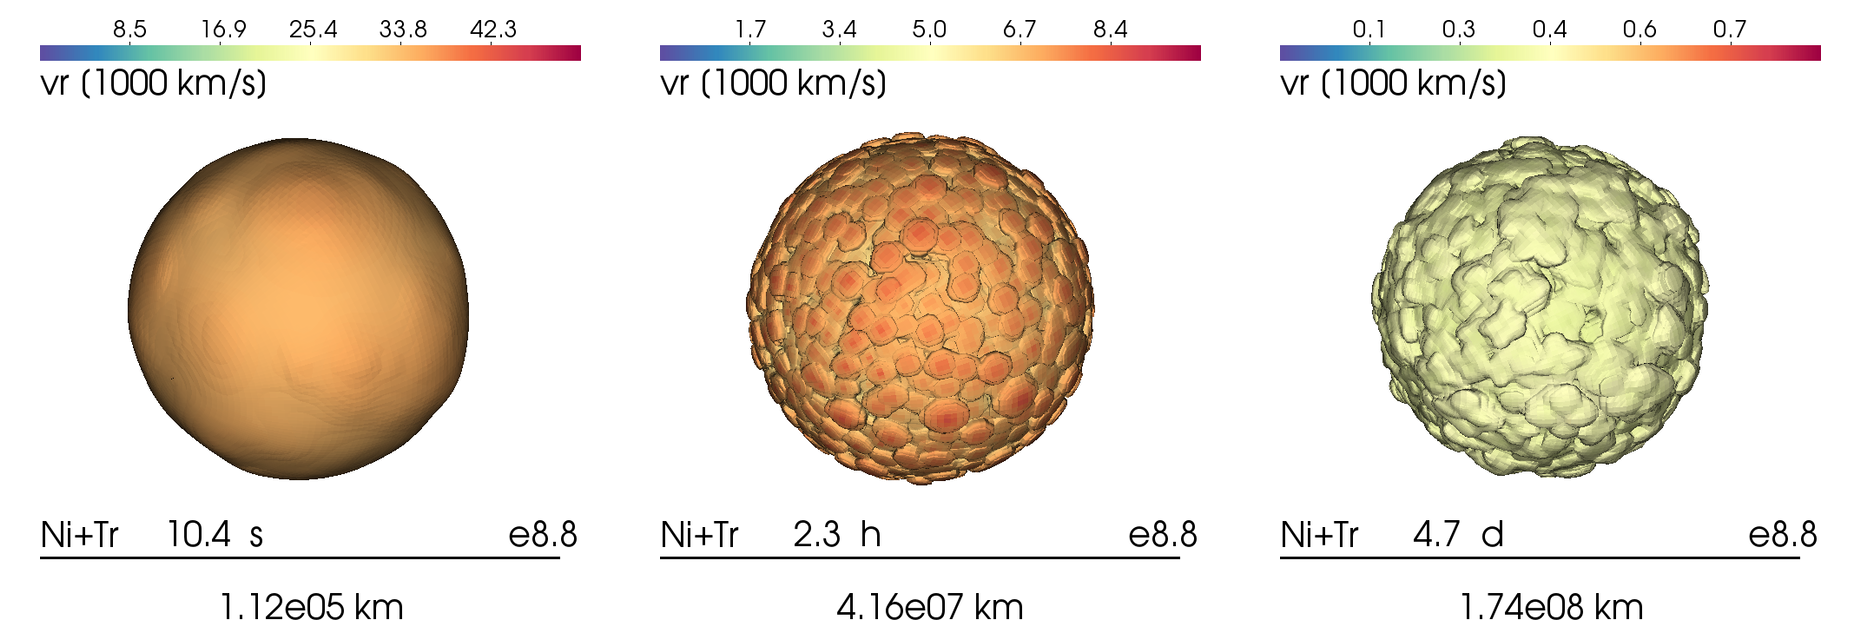
\includegraphics[width=\textwidth]{pic/e8_tile_1_3.png}
    \caption{3D renderings of the $X_{\nickel\mathord{+}\tracer}\mathord{=}0.03$ 
             iso-surface of model \onemg at the indicated times. Color-coding represents the radial velocity of the material. From the initially spherical distribution of the neutrino-heated ejecta we observe the growth of small scale RT plumes. Due to the early formation of the reverse shock and spherical initial conditions of the explosion (see text for details) the final configuration of the neutrino-heated ejecta is basically spherical. }
\label{fig:e8 3d rendering}
\end{figure*}% ---------------


Exactly as in the 1D simulation, the CO and He layers are compressed into a dense shell,
just behind the supernova shock. The dense shell is located at a radius of 
$\mathord{\approx}2\times 10^4\,\rm km$ at $\tpb\mathord{=}0.5\,\s$ (
see Figure~\ref{fig:density profiles all times} and Figure~\ref{fig:e8 rho cuts}).
Already at $\tpb\mathord{\approx}1.5\,\s$, a reverse shock forms at the bottom 
of the dense shell (see thin yellow shell in Figure~\ref{fig:e8 rho cuts} at $10\,\s$) .
By this time the bulk of the neutrino-heated ejecta has expanded in the region
inside $\approx 1.5\times 10^5\,\rm km$.
While this innermost metal-rich material seems to expand in a basically self-similar fashion
(see similarity of the snapshots until $\tpb=150\,\s$ in Figure~\ref{fig:e8 nix cuts}),
the growth of the RTI in small cusps in the unstable layer around the He/H interface 
(located between the dense shell and the forward shock) begin to fragment the top of 
the dense shell (compare panel at $\tpb\mathord{\approx} 150\,\s $ in Figure~\ref{fig:e8 rho cuts}). At $\tpb=300\,\s$,
the metal-rich ejecta catch up with the expanding dense shell and are strongly decelerated.

In consequence, the higher entropy/lower density plumes are compressed to flat
structures while the (higher density) regions in between the plumes are able 
to penetrate the dense shell, thereby inducing small perturbations at this interface. 
Superimposed on these perturbations, RT plumes grow over the following $\approx 1100\,\s$ 
around the mass shell of the He/H interface, mixing clumps of the outermost 
\nickel-rich layer outward into the carbon and helium rich layers.

The reverse shock, which is visible at $\tpb=2.3\,\text{h}$ in 
Figure~\ref{fig:e8 nix cuts} as the yellow to red discontinuity, 
begins to propagate back in radius, thereby 
compressing the innermost ejecta.
At $\tpb\mathrm{\approx }10\,\text{h}$ the passage of the reverse shock and 
the growth of the RTI has fully erased any trace of the initial structures 
present at the onset of the explosion. 
However, the overall morphology of the neutrino-heated ejecta is still essentially spherical.

% z9.6
\begin{figure*}% Figure z9.6 NiX
 \centering
 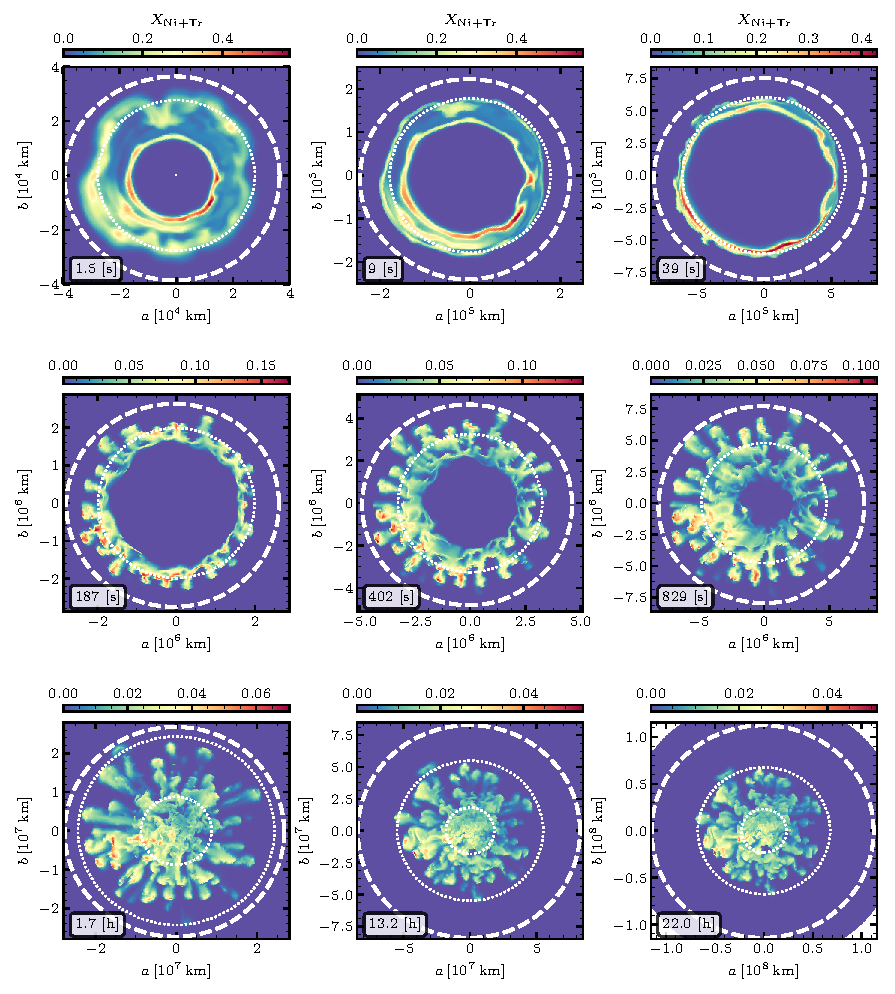
\includegraphics[width=\textwidth,trim=0cm 0.0cm 0cm 0cm,clip]{pic/z9_3d_3x3_NiX.pdf}
 \caption{Slices of the $\nickel+\tracer$ mass fraction of the 3D simulation of model
        \znine at the indicated times.  Cyan colored regions represent the atmosphere of the progenitor. 
   The initial asymmetries that developed during the onset of explosion are still visible at $\tpb\mathord{=}1.5\,\s$,
   but are soon compressed to flat structures as they encounter the RT unstable dense shell behind the CO/He interface
   (see times from $\tpb\mathord{=}9\,\s$ to $\tpb\mathord{=}39\,s$). 
   Over the next, roughly, one hour, the growing RTI mixes the outer \nickel rich layers outwards in mass coordinate in numerous 
   small fingers.
   $1.7\,\rm h$ after bounce the RTI has basically saturated. The final morphology of the \nickel-rich ejecta has lost every
   resemblance with the state at $t_{\mathrm{map}}$ and is dominated by small scale structures. However, the overall 
   distribution of \nickel and \tracer remains basically spherical.
 }
 \label{fig:z9 nix cuts}
\end{figure*}% Figure z9.6 slices


\begin{figure*}% --------------- z9.6 FIGURE rho cuts 3d
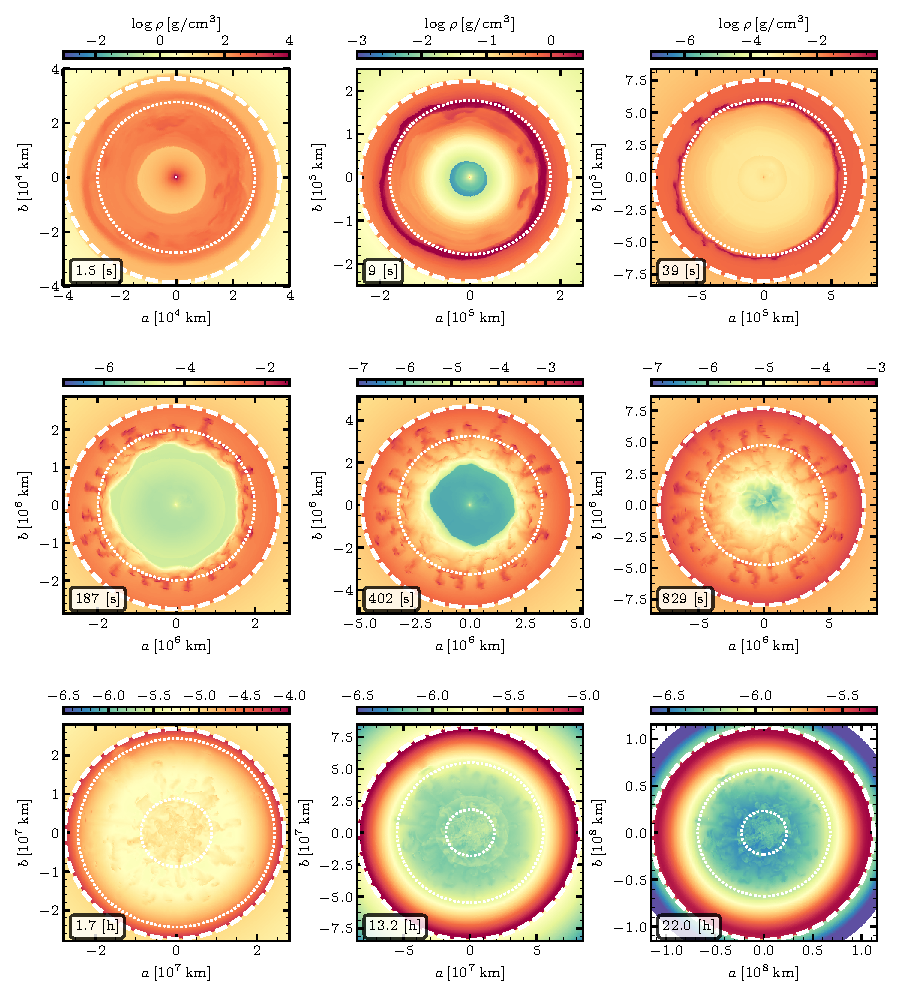
\includegraphics[width=\textwidth]{pic/z9_3d_3x3_den.pdf}
    \caption{Slices showing the density in the 3D simulation of model \znine 
        at the indicated times. 
    The dashed white line indicates the shock radius while the dotted white 
    lines indicate the mass-shell CO/He and He/H interfaces.  Cyan colored regions represent the atmosphere of the progenitor. 
    Passage of the CO/He interface lead to the formation of a dense shell 
    and a reverse shock
    visible as the orange discontinuity at $\tpb\mathord{\approx}2.3\,\s$. Over the 
    next $\mathord{\approx}40\,\s$ RT plumes
    start to grow within the unstable region between the shocks thereby fragmenting
    the dense shell.
    As the reverse shock propagates back in radius, similar to the 
    results presented for model \onemg, the plumes
    grow to their maximal radial extent 
    (see panels at $\tpb\mathord{=}187\,\s-829\,\s$).
    The final morphology of the ejecta at $\tpb\mathord{\approx}22\,\mathrm{h}$ resembles 
    the late time morphology in model \onemg}
\label{fig:z9 rho cuts}
\end{figure*}% ---------------

In Figure~\ref{fig:z9 nix cuts}, we show slices of the $\nickel\mathord{+}\tracer\,$  mass-fraction in the 3D simulation of model \znine. 
The dashed white dashed line indicates the shock radius while the dotted lines indicate the positions of 
the mass-shells of the CO/He and He/H interfaces.
The dense shell which forms after the forward shock crossed 
the CO/He interface (see Figure~\ref{fig:density profiles all times}) 
is visible as the round light red region with a radius of $r\mathrm{\approx} 4\times 10^4\,\mathrm{km}$ 
in Figure \ref{fig:z9 rho cuts}.  

Within the first $\mathord{\approx}10\,\s$ the fastest of the 
neutrino-heated ejecta encounter this dense CO-rich shell (see Figure~\ref{fig:z9 nix cuts})
and are compressed and squeezed to flat structures around $30\,\s$ later.
Similar to the results presented for the \onemg model, the slightly over-dense regions between the high 
entropy plumes induce long wavelength perturbations as they deform and 
try to penetrate the RT unstable dense shell. 
Over the next few minutes, RT fingers grow on top of these deformations and fragment the 
dense shell into numerous \nickel-rich shrapnels.

\begin{figure*}% --------------- FIGURE z9.6 3d rendering
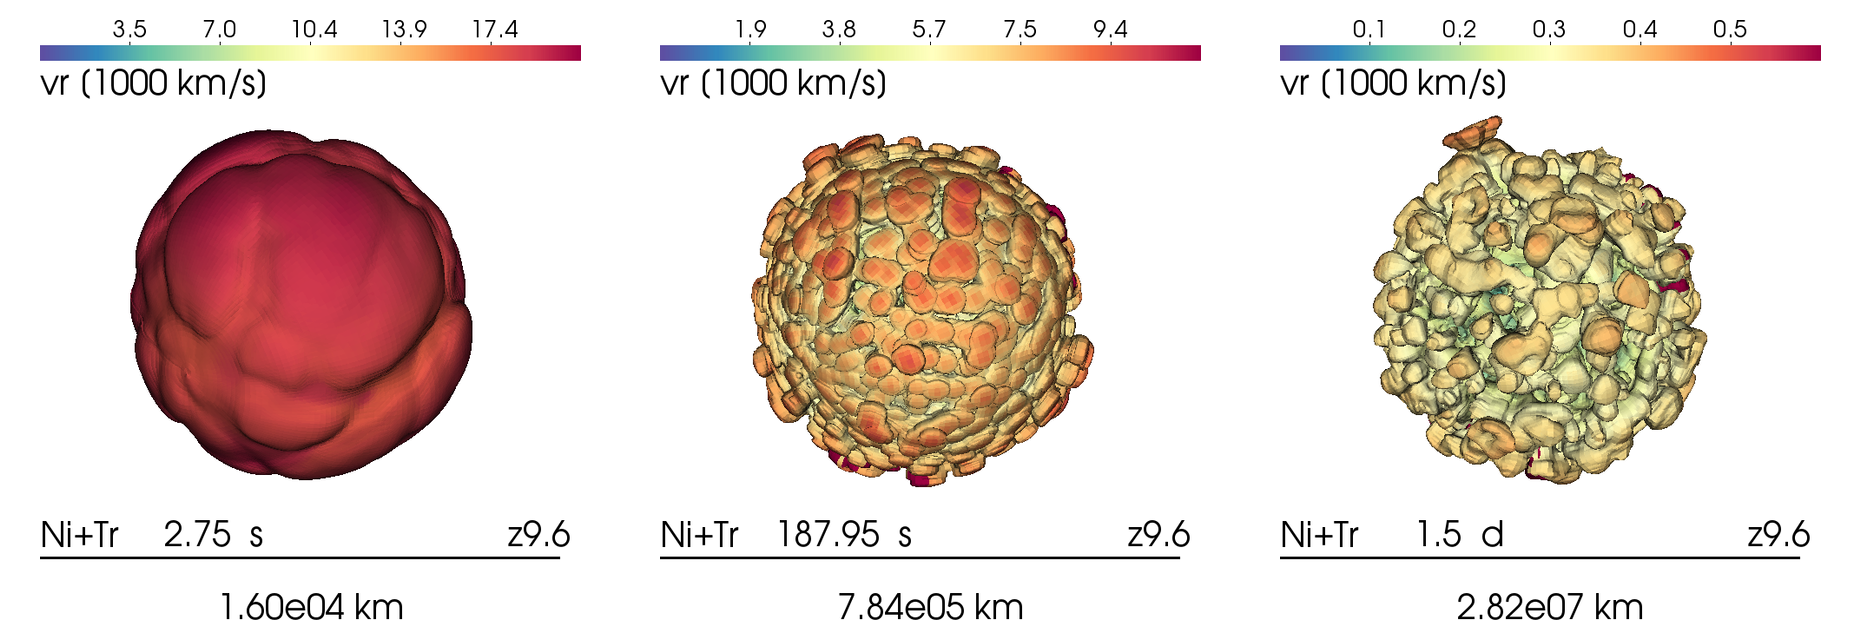
\includegraphics[width=\textwidth]{pic/z9_tile_1_3.png}
    \caption{3D renderings of the $X_{\nickel\mathord{+}\tracer}\mathord{=}0.03$ 
             iso-surface of model \znine at the indicated times.  Color-coding represents the radial velocity of the material. We find the growth of small scale (high $\ell$ number) RT plumes on top of the initial asymmetries of the explosion. Early formation of the reverse shock already in the He-core, the small scale initial asymmetries and the small size of the RT unstable layer prevent efficient growth of the RTI, leaving the final state basically spherical. }
\label{fig:z9 3d rendering}
\end{figure*}% ---------------
While the fingers grow progressively, the reverse shock (visible as the green to blue discontinuity 
at $\tpb=187\,\s$ in Figure~\ref{fig:z9 nix cuts}) begins to propagate back in radius. 
At $\tpb=829\,\s$ the reverse shock reaches the center of our numerical grid having 
compressed and decelerated the innermost material. 
At $\tpb=1.7\,\rm h$, the forward shock has crossed the He/H interface and the inner 
material has been fully shredded by the instability.

As the shock does not show any significant change in velocity at the interface, we observe 
no additional growth of the RTI nor the formation of a reverse shock.
Thus, the morphology of the innermost ejecta seems to be determined early on, already 
before the shock crosses the He/H interface.

Comparing the distribution of \nickel and \tracer of model \onemg 
(Figure~\ref{fig:e8 nix cuts}) model \znine (Figure~\ref{fig:z9 nix cuts}) 
shortly before shock breakout we find a slightly more clumped morphology in the 
$9.6\,\solm$ progenitor. However, the morphology of the neutrino-heated ejecta in 
model \znine also remains basically spherical.

% s9.0
The evolution of the neutrino-heated ejecta of model \snine proceeds drastically different to the ECSNe-like progenitors. 
As discussed in Section~\ref{sec:Evolution during the first second}, 
the initial asymmetries and shock deformation seen in model \snine are 
considerably larger than found in the ECSNe-like models. Strong convection leads to the formation of a large metal-rich plume which travels about two times 
faster than the surrounding material at the time of shock-revival ($\tpb\mathord{\approx} 0.5\,\s$).  
It crosses the CO/He interface of the star at $\tpb\mathord{\approx}1.3\,\s$, 
shortly after the forward shock. In comparison, the slowest 
moving material reaches the interface around $ 0.65\,\s$ later. 

\begin{figure*}% --------------- s9.0 FIGURE species cuts 3d
\centering
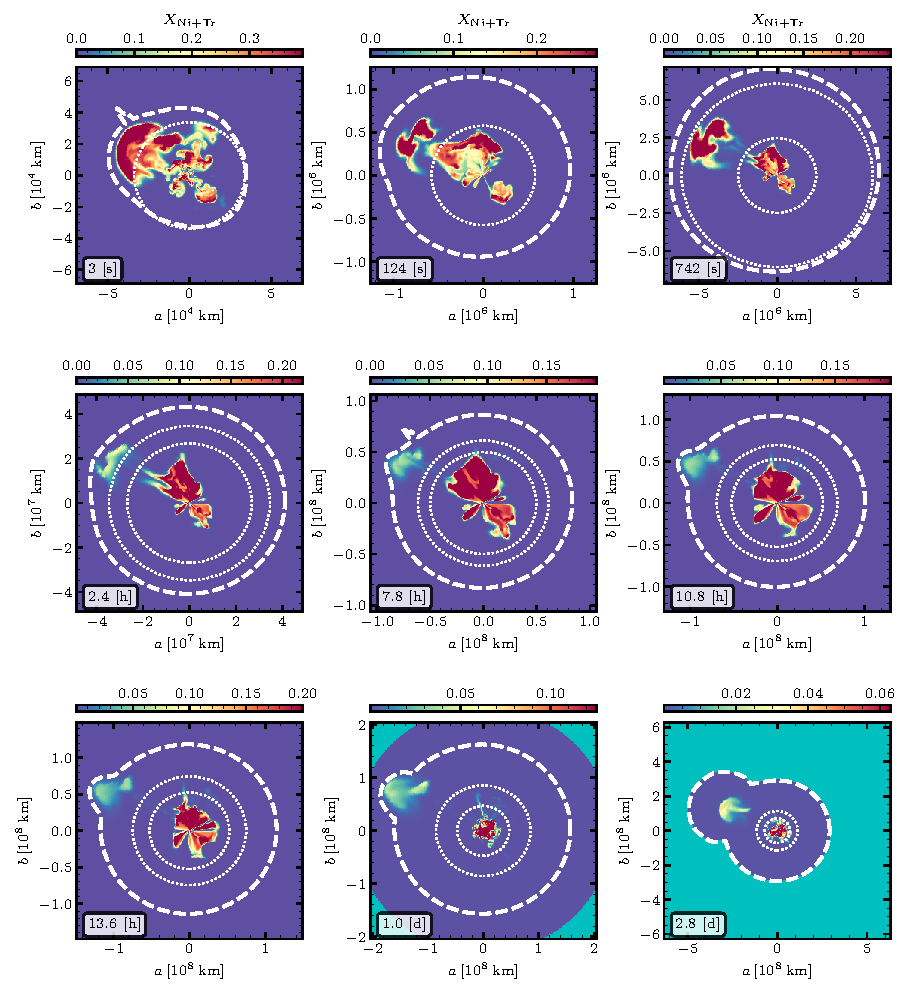
\includegraphics[width=\textwidth]{pic/s9_3d_3x3_NiX.pdf}
    \caption{Slices of the $\nickel+\tracer$ mass fraction of model \snine at the indicated times. The dashed white line indicates the shock radius while the dotted white 
    lines indicate the mass-shell CO/He and He/H interfaces. Cyan colored regions represent the atmosphere of the progenitor. 
    The $\nickel\mathord{+}\tracer$ distribution underlines the connection between the initial asymmetries and the 
    large clump shortly before shock breakout. 
    At $\tpb\mathord{=}3\,\s$ most of the \nickel-rich material is ejected in the 10 o'clock direction. While
    the innermost ejecta are compressed and decelerated by the dense shells and reverse shocks that 
    form at the CO/He and He/H interface, the large clump escapes strong deceleration and even deforms the 
    otherwise spherical shockwave shortly before breakout.
    }
\label{fig:s9 nix cuts}
\end{figure*}% ---------------

The crossing of the CO/He interface by the shockwave has several dynamical consequences. 
Due to the increasing $\rho r^3$ behind the interface, the shock is 
decelerated and sends a pressure wave back into the ejecta. Consequently, 
the post-shock matter is compressed into a
dense shell. This high-density region is aspherical,
in contrast to the shells found in the ECSNe-like progenitors, which is due to the still  
deformed supernova shock (see first two panels in Figure~\ref{fig:s9 rho cuts} 
from  $\tpb\mathord{=}3\,\s-124\,\s$).

Around the dense shell we observe the growth of large plumes which stem from the initial 
asymmetries of the explosion. These can be seen in 10 o'clock direction in
Figure~\ref{fig:s9 nix cuts} at $\tpb\mathord{\approx} 124\,\s$ and Figure~\ref{fig:s9 3d rendering}.
At the top of these plumes small RTI fingers grow, in line with the analysis of the amplification factors presented in Section~\ref{sec:Linear stability analysis}. 
Note that at this point in time the still deformed supernova shock crosses the He/H interface.

Due to the varying $\rho r^3$ around this composition interface, the shock decelerates and accelerates, thereby forming a dense shell (see yellow shell in Figure~\ref{fig:s9 rho cuts} at $\tpb\mathord{\approx}740\,\s$). 

\begin{figure*}% --------------- s9.0 FIGURE rho cuts 3d
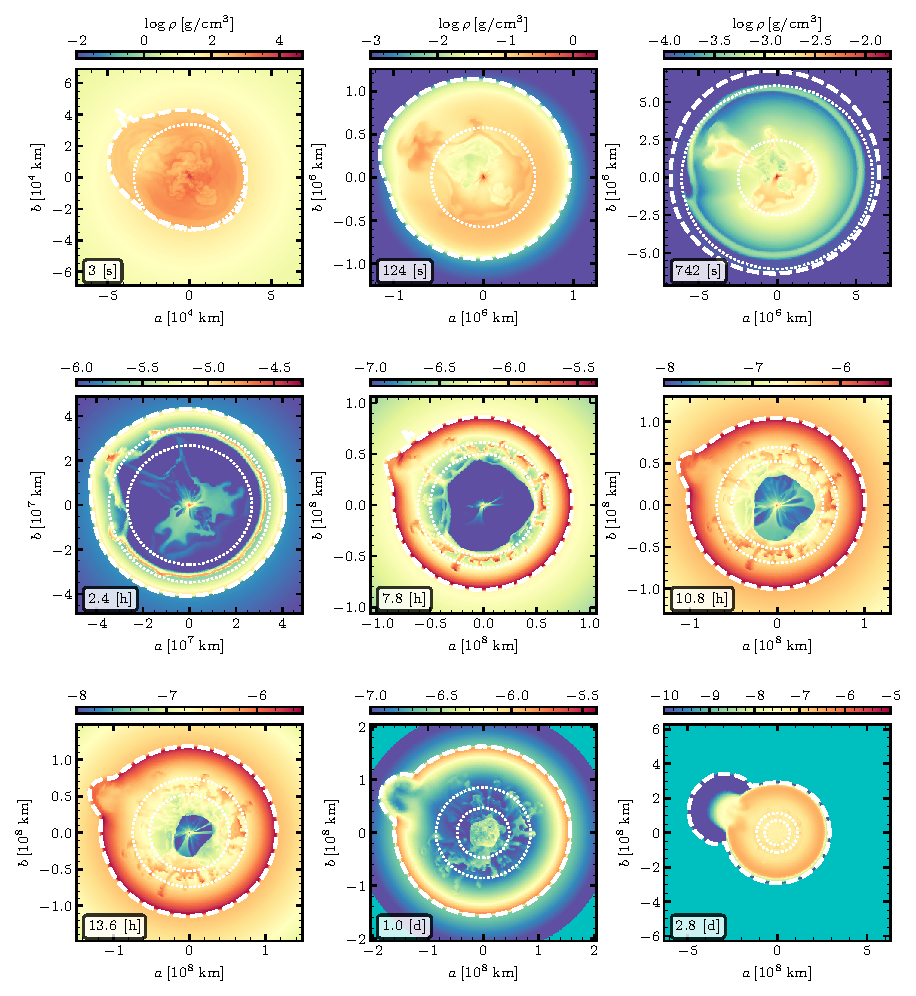
\includegraphics[width=\textwidth]{pic/s9_3d_3x3_den.pdf}
    \caption{Slices of the density of model \snine at the indicated times. 
        The dashed white line indicates the shock radius while the 
        dotted white lines indicate the CO/He and He/H interfaces.  Cyan colored regions represent the atmosphere of the progenitor.
        Different to the ECSNe-like progenitors we observe the growth of large 
        scale RT plumes caused by the large asymmetries at the onset of explosion.
        The seed for the largest plume seems to be set already at around $3\,s$ 
        after bounce when the shock passes the CO/He interface. We first observe
        the growth of the RTI at the top of the largest and fastest initial convective plume 
        (see e.g. $\tpb\mathord{=}124\,\s$ in 10 o'clock direction) 
        and only moderate deceleration of the same.
        Shortly afterwards the plume arrives at the unstable He/H interface 
        inducing a large scale perturbation.
        While the slower RTI plumes are decelerated by the reverse shock that formed 
        at the He/H interface, the large
        clump drives the shock to larger radii, thereby transporting a 
        significant amount of neutrino-heated ejecta to large velocities.
    }
\label{fig:s9 rho cuts}
\end{figure*}% ---------------

When the fast and dense metal-rich plume encounters the shell, it induces a high amplitude perturbation at this RT unstable layer. 
From this perturbation, aided by the large initial momentum of the metal-rich plume, we observe the growth of a large RT plume. As matter is accelerated by the instability to higher velocities than the speed of the shock, the plume is able to deform the forward shock in its trajectory (compare Figure~\ref{fig:s9 rho cuts} at $\tpb\mathord{\geq}2.4\,\rm h$).

Concurrently, the reverse shock, which forms at the bottom of the He/H interface, 
propagates back into the ejecta and strongly decelerates and compresses the 
$\nickel\mathord{+}\tracer$ rich material close to the center 
(see Figure~\ref{fig:s9 rho cuts} at $\tpb\mathord{\approx}7.8\rm h$). 
The growing RTI around the CO/He interface (clearly visible in Figure~\ref{fig:s9 rho cuts} at
$\tpb\mathord{\approx}7.8\rm h$)
seems to only slightly affect the outer boundary of the inner $\nickel\mathord{+}\tracer$-rich
material, as can be seen in Figure~\ref{fig:s9 nix cuts} at $\tpb\mathord{\geq}7.8\rm h$ (in
line with the small amplification factors found in this region).

\begin{figure*}% --------------- FIGURE s9.0 3d rendering
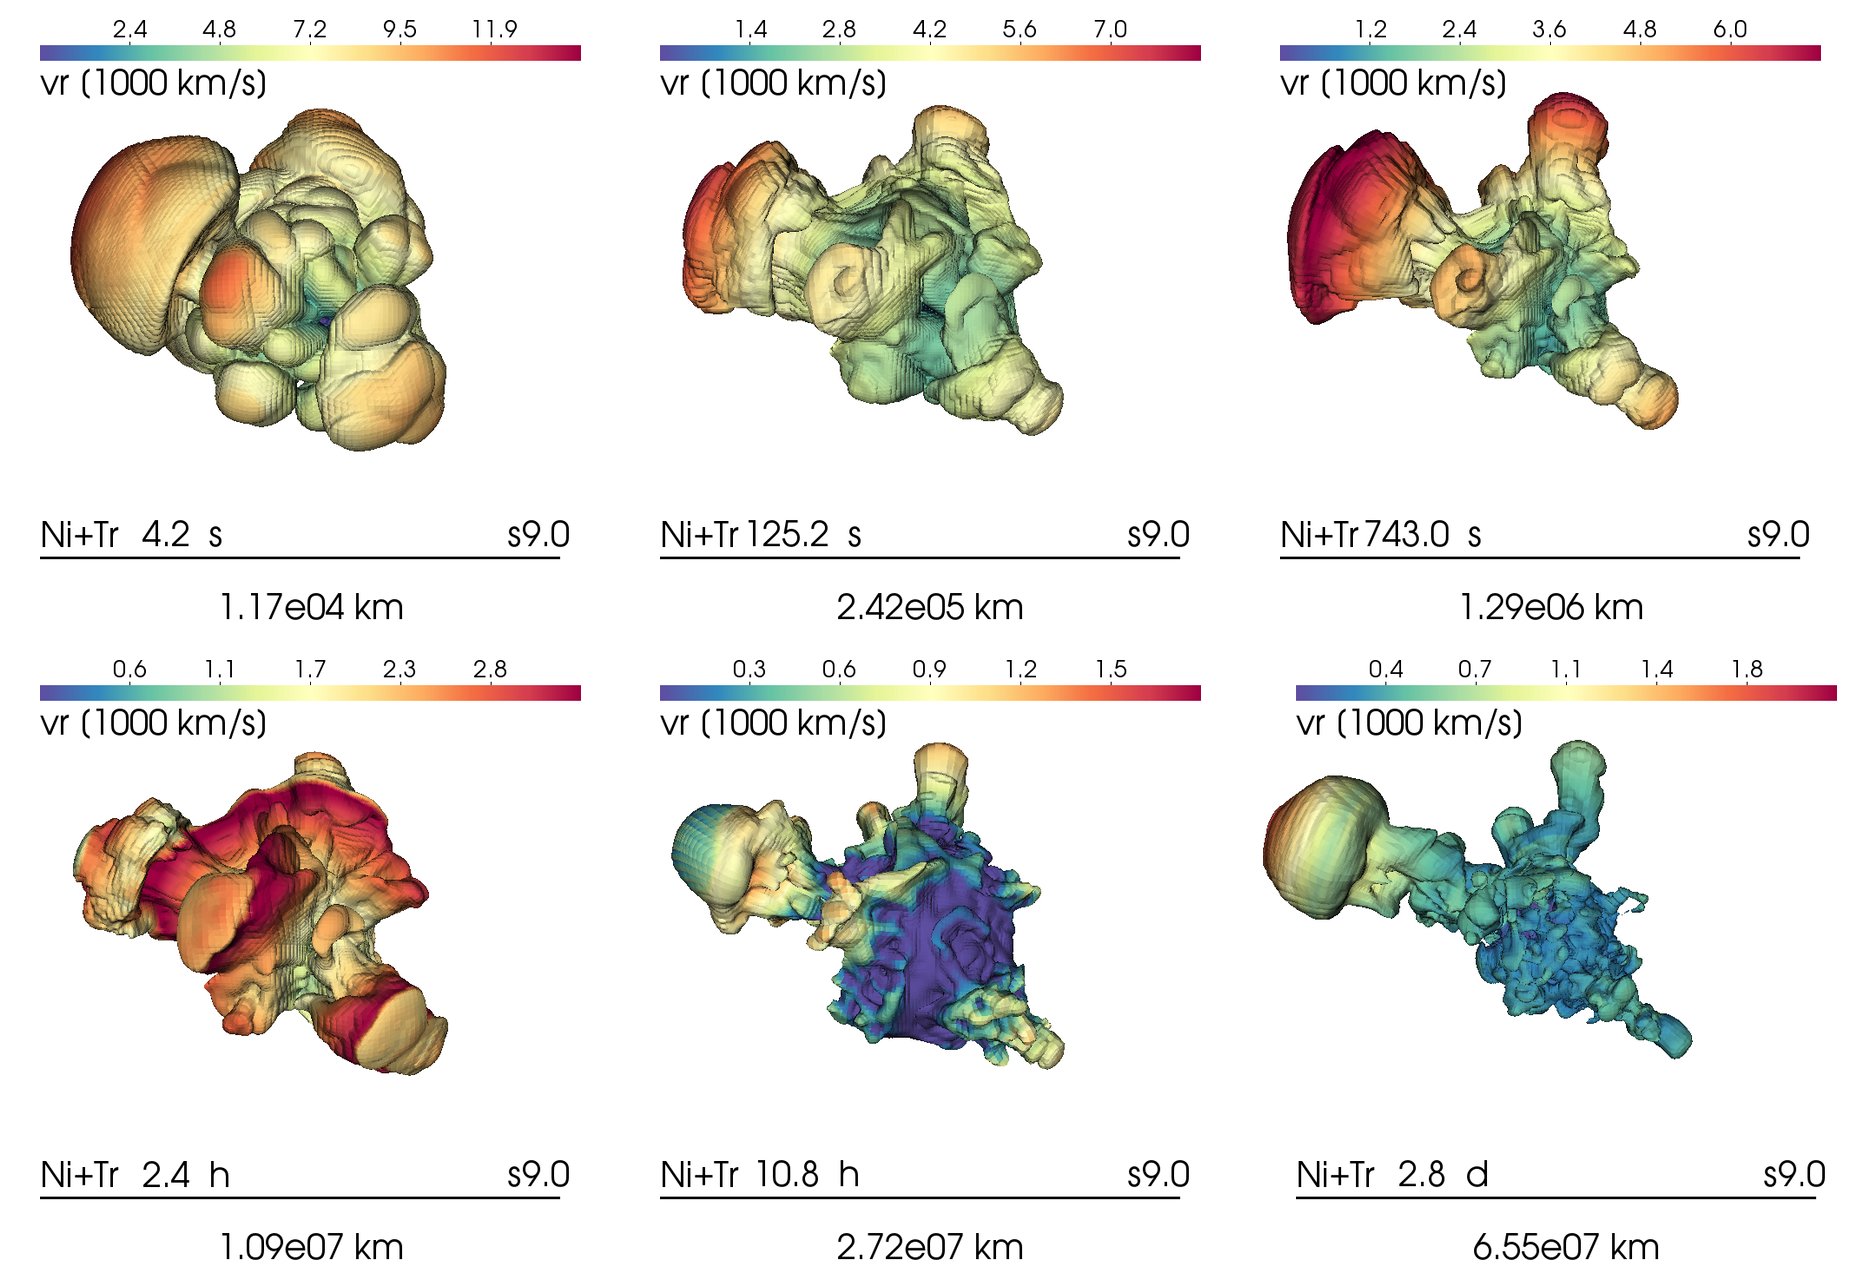
\includegraphics[width=\textwidth]{pic/s9_tile_2_3.png}
    \caption{3D renderings of the $X_{\nickel\mathord{+}\tracer}\mathord{=}0.03$ 
             iso-surface of model \snine at the indicated times. Color-coding represents the radial velocity of the material. During the first roughly $800\,\s$ the largest initial asymmetries grow to large metal rich plumes, while the innermost matter is compressed by the dense shell around the CO/He interface. In the following, these fastest plumes encounter the dense shell behind the He/H and induce large amplitude perturbations at the RT unstable layer. Consequently, large metal rich RT fingers begin to grow from the interface. At $\tpb\mathord{=}2.8\,\rm d$ we find one very large and two smaller metal-rich plumes which penetrate the surface of the star even ahead of the average shock radius.}
\label{fig:s9 3d rendering}
\end{figure*}% ---------------

Due to the strong compression of the innermost material, the fast plume almost fully detaches from the core material as it propagates through the hydrogen envelope of the star (see last two panels in Figure~\ref{fig:s9 3d rendering}).
It encounters the surface of the star at around $\tpb \mathord{\approx} 1.6\, d$, so almost $1\,\rm d$ earlier than the angle-averaged shock.
Why is the large plume able to travel with such high velocities, even deforming the forward shock, while the bulk of material travels at considerable slower speed?
Firstly, the fastest $\nickel\mathord{+}\tracer$ material is, at all times, in close vicinity of the immediate post-shock matter (see Figure~\ref{fig:radii all times}). 
Further, after the forward shock has crossed the He/H interface, this material is decelerated less than the average shock, since the material encounters a less steep density profile.
Additionally, large growth rates at the He/H interface lead to an efficient acceleration of material within the unstable layers, which also escape the strong deceleration by the reverse shock.
In consequence, the $\nickel\mathord{+}\tracer$-rich plume catches up with the forward shock in the hydrogen envelope. Due to its large momentum it deforms the outgoing forward shock in its trajectory. \COM{Buoancy forces ?}
This is similar as observed in model \onemg, where the basically spherically distributed neutrino-heated ejecta catch up with the strongly decelerated immediate post-shock material, thereby accelerating the forward shock (see Figure~\ref{fig:radii all times}).

\subsection{Extent of mixing}

\begin{figure*}% Figure mass distribution at sbo
 \centering
 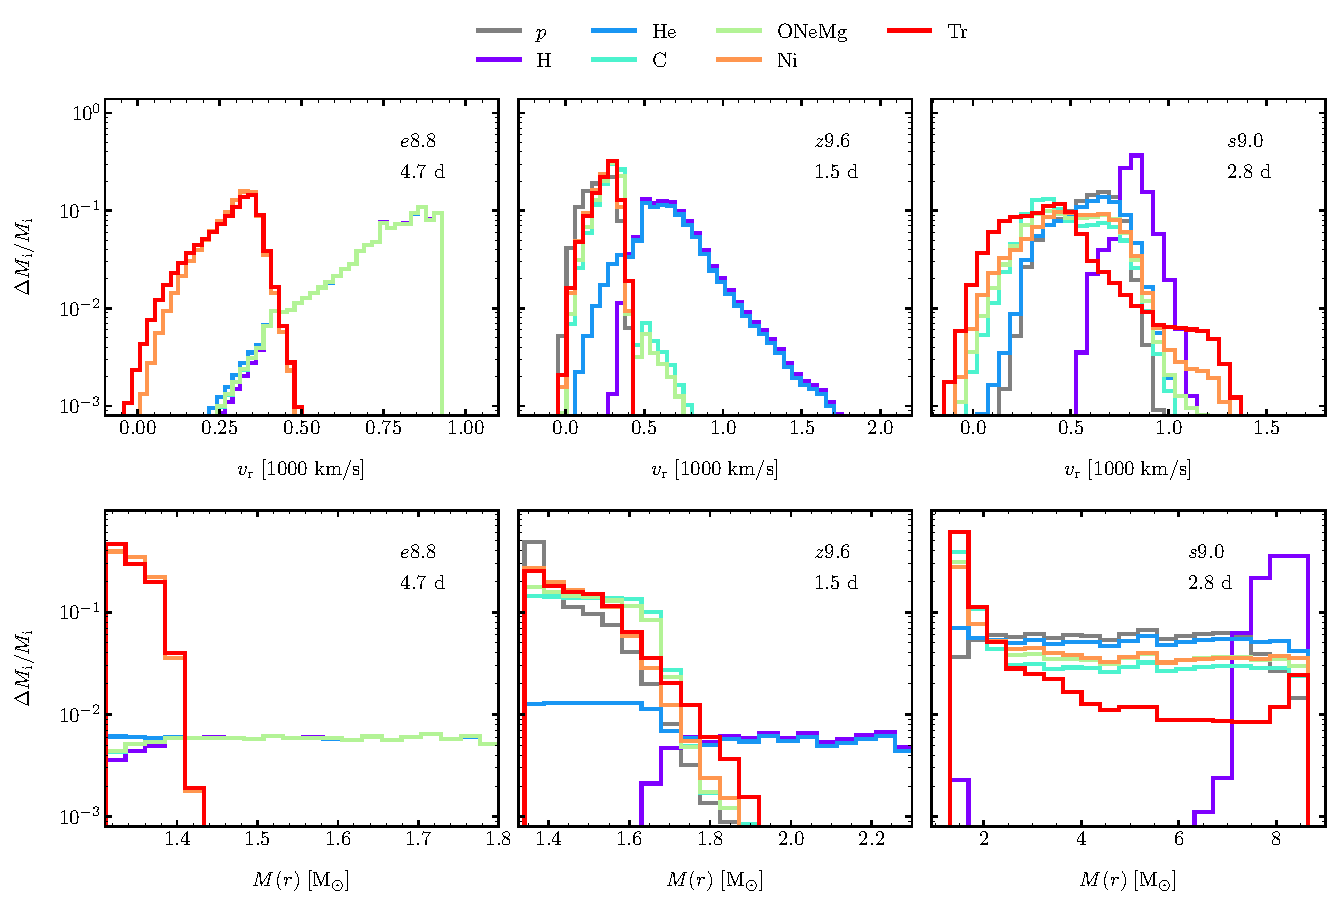
\includegraphics[width=\textwidth,trim=0cm 0.0cm 0cm 0cm, clip]{pic/z96_s9_e8_3d_massDis_mvr_and_masstime_sbo_paper.pdf}
 \caption{Mass distributions of elements versus radial velocity (top row) and enclosed mass (bottom row) for all our models at the time of shock breakout. We use 50 bins in velocity space covering and 30 bins in mass space, where we restrict the analysis of models \onemg and \znine to $1.8\,\solm$ and $2.3\,\solm$ respectively, since mixing of the neutrino-heated ejecta beyond these mass-shells is insignificant. For model \snine we consider the whole computational domain for our analysis.
 The ECSNe-like models (\onemg and \znine) only mix a tiny amount of \nickel into the bottom of the H-envelope, whereas vigorous mixing in model \snine transports a significant amount of 
 neutrino-heated ejecta to large mass coordinates.}
 \label{fig:mass distribution sbo}
\end{figure*}

In Figure~\ref{fig:mass distribution sbo} we display the mass distributions of free protons/hydrogen, helium, carbon, oxygen-neon-magnesium, nickel and the tracer nucleus for all our models at the time of shock breakout as functions of radial velocity as mass coordinate. 
The distributions of the iron-rich ejecta of the ECSNe-like models (\onemg and \znine) have similar shapes in velocity and mass coordinate (apart from the differences that result from the different initial progenitor composition). 

They are characterized by a maximum centred around $0.25\mathord{\times}10^3\,\kms$ and have a high-velocity tail which extends to $\mathord{\sim}0.45\mathord{\times}10^3\,\kms$ (using $\Delta M_{\mathrm{i}}/ M_{\mathrm{i}}\mathord{=}4\mathord{\times}10^{-4}$ as a threshold value). The mixing in velocity space corresponds to mixing in mass coordinate to a maximum of $\mathord{\sim}1.4\,\solm$ in model \onemg and $\mathord{\sim}2\,\solm$ in model \znine so only to the bottom of the respective hydrogen envelope. 

Why is the mixing more efficient in model \znine in comparison to model \onemg although the explosion energy and the integrated growth factors are larger in the latter? 
The answer can be found in inspecting Figures~\ref{fig:mdp first mapping} and 
\ref{fig:density profiles all times}. 
Model \znine already shows more efficient mixing at the onset of explosion. 
Additionally, the density profile of model \znine exhibits less extreme drops outside the Si/CO and CO/He interfaces than the sharp drop in density in the ECSN progenitor. 
Thus, shock deceleration is less severe and the formation of the reverse shock is 
delayed enabling more efficient mixing while the forward shock runs through the 
helium-shell of model \znine.

In contrast, heavy elements are mixed to large mass coordinates and velocities in model \snine.
This is facilitated by the large initial asymmetries at the onset of explosion.
Fast metal-rich plumes escape the deceleration at the CO/He interface and reverse shock formation in the H-envelope thereby transporting a significant amount of the total $\nickel\mathord{+}\tracer$ mass to large mass coordinates.
Mixing of intermediate mass elements is driven by the growth of the RTI which causes a fragmentation of the dense shells which form after the forward shock crosses the CO/He and He/H interfaces.
Most importantly, the large plume is able to transport $\nickel\mathord{+}\tracer$-rich matter to large velocities and mass coordinates. We find around $4\%$ of the
$\nickel\mathord{+}\tracer$-rich material travels with more than $1,000\,\kms$ and thus ahead of the bulk of metal-rich matter.

\subsection{Dependence on the explosion energy}
\label{sec:Dependence on the explosion energy}

\begin{figure*}% e8.8 2d mass dis sbo
 \centering
 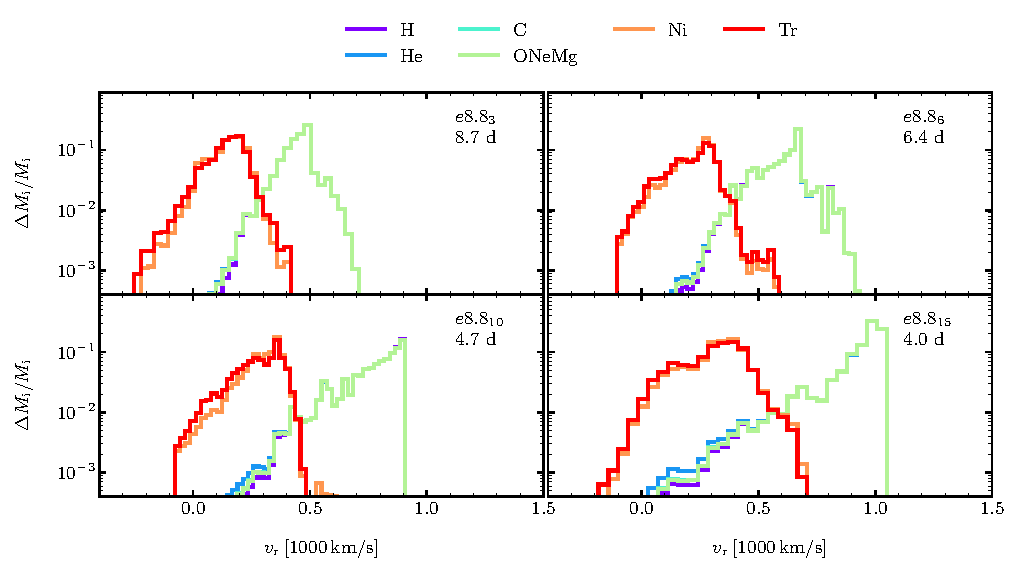
\includegraphics[width=0.95\textwidth]{pic/e8_2d_all_sbo_massdis_velocity.pdf}
 \caption{Mass distribution of the 2D simulations of model \onemg using the calibrations as listed in Table~\ref{table:e8param} at the time of shock-breakout. Maximum velocities, and thus also the velocities of the bulk of \nickel and \tracer, scale with $\sqrt{E_{\mathrm{exp}}}$ leading to slightly enhanced mixing for more energetic models. }
 \label{fig:e8 2d massDis sbo}
\end{figure*}
In Figure~\ref{fig:e8 2d massDis sbo} we show the mass distributions as a function of radial velocity for the 2D simulations of model \onemg, using the calibrations as listed in Table~\ref{table:e8param}, at the time of shock-breakout. 

Comparing the distributions of model $e8.8_{10}^{\mathrm{2D}}$ with the 3D simulation, the efficiency of mixing in model \onemg does not seem to be significantly dependent on the chosen dimensionality. This thus enables us to investigate the influence of the explosion energy on the efficiency of mixing in our 2D simulations of model \onemg.
 
Inspecting Figure~\ref{fig:e8 2d massDis sbo}, we find that the bulk of \nickel resides at low velocities of $\mathord{\sim}0.17\mathord{-}0.40\mathord{\times}10^3\,\kms$ increasing with explosion energy as $v_{r}\mathord{\sim}\sqrt{E_{\mathrm{exp}}}$. 
For larger explosion energies the downward mixing (to smaller velocities) of lighter elements also seem to be more efficient, but the effect is small and affects only $\mathord{<}1\%$ of the respective elements. 

The mixing in velocity space corresponds to a distribution of \nickel and \tracer to a maximum mass coordinate of $1.37\mathord{-}1.436\,\solm$ also increasing with explosion energy, again using $\Delta M/M\mathord{=}4\mathord{\times}10^{-4}$ as a threshold value. Note that the 4.49 \solm hydrogen envelope of the progenitor initially extended from 1.34 \solm to 5.83 \solm, thus mixing only affects the innermost part of the envelope.

% iron cores
As the ion core progenitors are exploded self consistently their explosion energy is fixed within our framework. Drawing direct connections between the amount of mixing and the explosion energy can therefore not be done. Comparing the \znine model with electron-capture model, that have similar explosion energies, hints that the influence is, however, minor. Decisive for the amount of nickel mixing is the progenitor structure and initial perturbations after shock revival. This view is supported by the strong mixing apparent in model \snine that has comparable explosion energy as well. The initial density perturbations combined with the strong de- and acceleration of the forward shock in the envelope of the progenitor yields high growth-rates over a larger space in mass coordinate. 


\section{Comparison to previous studies}
\label{sec:Comparison to previous studies}

Previous studies like the ones of \cite{Hammer2010}, \citet{Wongwathanarat2015}, \citet{Kifonidis2006} also performed simulations of the long-time evolution of CCSNe after shock-revival based on 2D/3D initial data. These studies employed RSG and BSG progenitors as a proxy for Sanduleak -69 202, the progenitor of SN1987A. \citet{Hammer2010} used a 15 \solm blue supergiant, while \citet{Wongwathanarat2015}  deployed various models from 15-20 \solm. 
These more massive progenitors differ strongly in their $\rho r^3$-profiles when compared to our ECSNe-like models. However, model \snine exhibits similar structural features (e.g. a significant variation of the density at the He/H interface) as the RSG models of Wo15.

The structural differences and similarities are reflected in the evaluation of the linear growth-rates of the RTI as shown in Figure~\ref{fig:growth rates}. While the ECSNe-like models show only small regions of possible RTI growth, model \snine exhibits similar amplitudes of the amplification factors and similar size of the affected regions as the models presented Wo15. Additionally, when the reverse shock in model \snine falls back, the fragmentation of the neutrino-heated matter in the He-core of the star already mixed \nickel-rich shrapnels into the hydrogen envelope, which thereby escape the strong deceleration. 
Consequently, neutrino-heated material can be mixed deep into the hydrogen envelope. 
Du to the specific structure of the ECSNe-like models, mixing is very inefficient, making the explosion of these progenitors almost spherical events. Thus, these models are distinct from the explosion of other RSGs reported in the literature. 

\section{Conclusions and Outlook}
In this study we presented the results of two- and three-dimensional
 simulations of CCSNe connecting the seconds after bounce, shock 
 revival and shock breakout. We used three low-mass progenitors, 
 two RSGs that formed an iron core at the end of their life 
 (\znine, \snine) and a newly explored ECSN progenitor (\onemg). 

\begin{figure*}% Figure models final visit
 \centering
 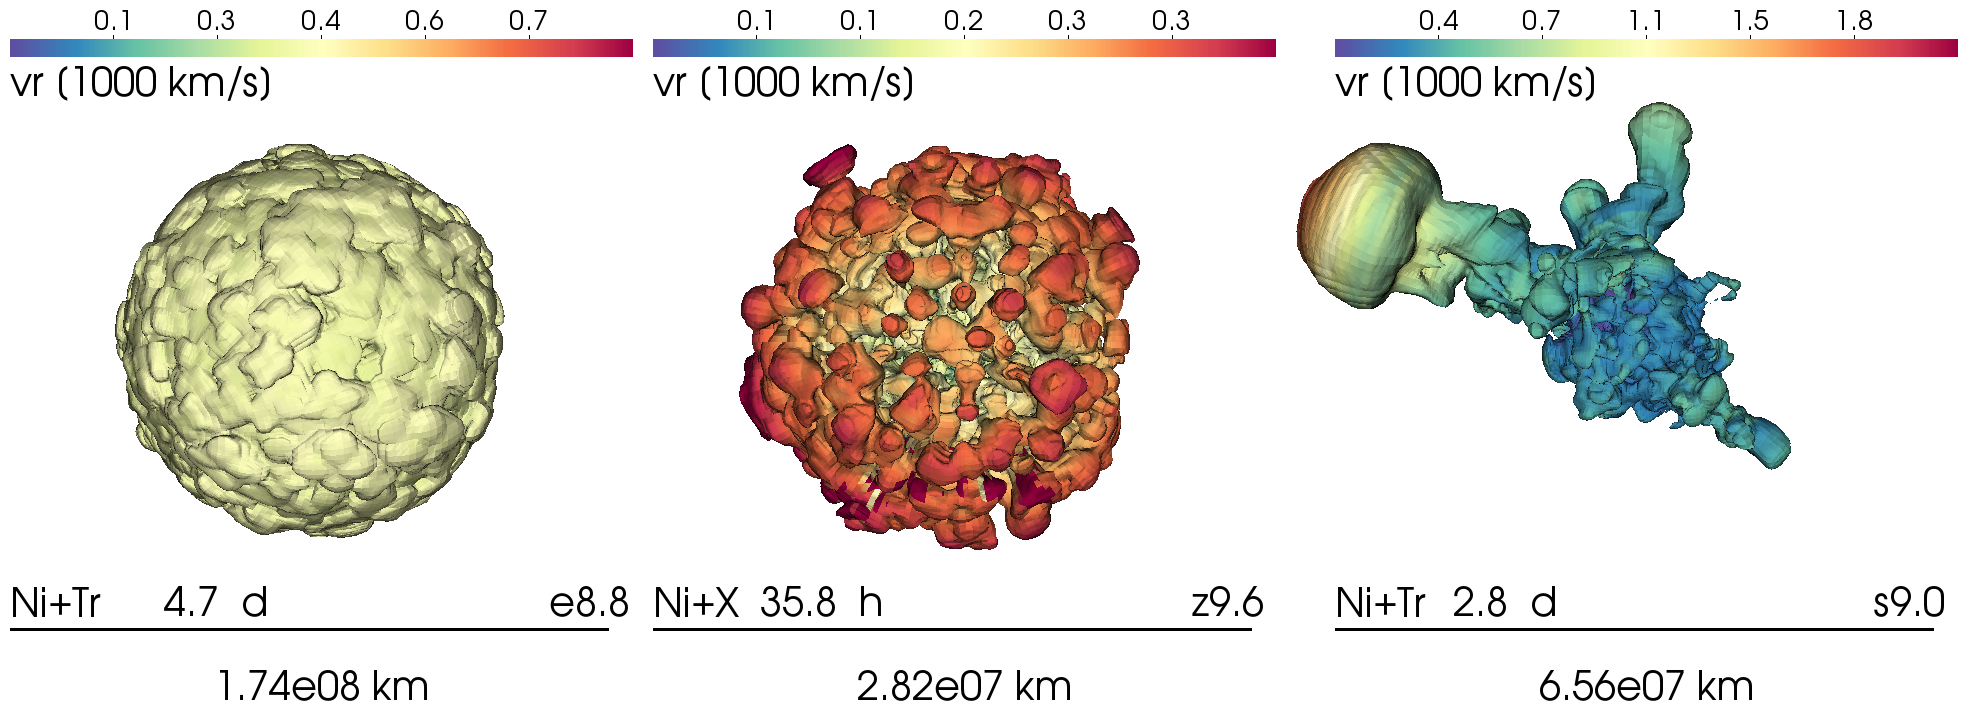
\includegraphics[width=\textwidth,trim=0cm 0.0cm 0cm 0cm,clip]{pic/visit_models.png}
 \caption{3D renderings of our models showing the $X_{\nickel\mathord{+}\tracer}\mathord{=}0.03$ iso-surface color-coded with the radial velocity at the time of shock breakout. Model \onemg remains almost perfectly spherical with only a few slightly extended RT fingers (9 o'clock and 3 o'clock directions in the left panel). Model \znine indeed shows numerous small RT fingers and a slightly stronger fragmentation of the ejecta than model \onemg, the overall morphology, however, remains nearly spherical. In contrast to the ECSNe-like models, model \snine shows strong deformations and large distinct RT fingers. 
 }
 \label{fig:all 3d models visit}
\end{figure*}% Figure VISIT

The explosion of the \onemg in one-, two- and three dimensions 
was initiated by imposing suitable values for neutrino luminosities 
and mean energies at the inner grid boundary located at a finite, 
time-dependent radius. Neutrino transport and neutrino-matter interactions 
were treated by the RbR gray neutrino transport scheme of \citet{Scheck2006}, 
including a improvement of the prescription for neutrino source 
terms as presented in the appendix. We confirmed the common behavior of 
ECSNe already presented in e.g. \citet{Kitaura2006,Gessner2018}. 
Early decline of the mass accretion rate leads to early explosions and 
fast shock expansion at the edge of the ONeMg core even in one-dimension. 
Shock trajectories are fairly independent of the chosen geometry, 
while the almost spherical expansion produces only small neutron 
star kicks of the order of a few \kms. Additionally convective 
motions in the multi-dimensional simulations are too weak and 
short-lasting to enable efficient mixing of neutrino-heated matter early on.

The immediate post bounce evolution of the iron core models was 
simulated with \vertex employing a fully self consistent neutrino 
transport scheme. A detailed analysis of the first second of 
evolution of model \znine is given in \citet{Melson2015a}, 
while simulations of model \snine as firstly presented in \citet{Melson2019}. 
In addition to these studies we showed the 
hydrodynamic neutron star kicks of these 
CCSN and investigated the morphology of the ejecta some 
hundred milliseconds after shock revival. 

When mass accretion subsides in all models and 
explosion energies and kick velocities begin to saturate 
we map the final state of our explosion simulations into \prom. 
This is achieved by excising the inner almost spherically symmetric 
regions of the previous simulations and replacing them by a 
suitable point mass. By incorporating the neutrino-driven wind
and setting the radius of the inner boundary below the sonic 
point we guarantee a seamless transition between the codes.

At the time when we continue the simulations of the explosions 
the forward shocks of all three dimensional models traveled 
already more than $10^4\;\mathrm{km}$. 
In order to aid us understand the formation of reverse shocks and
growth of RTI in the multi-dimensional models we appealed to spherically
symmetric simulations with the same setup starting from angle-averaged initial data
of the 3D post-bounce simulations.

The extremely steep density gradient at the core/envelope boundary
in model \onemg leads to rapid expansion 
of the shock until it crosses the He/H interface.
Thereafter, a featureless $\rho r^3$-profile leads to an untroubled 
propagation of the shock which is continuously decelerated.
The strong deceleration of the forward shock leads to the formation of a 
dense shell, below which a reverse shock forms already at $\tpb\mathord{\sim}1\,\s$.
In model \znine we observe the formation of a reverse shock also fairly early at
$\tpb\mathord{\sim}100\,\s$ after the shock crossed the CO/He interface.
The successive expansion of the shock, however, is untroubled due to the 
monotonic $\rho r^3$-profile.
The shock propagation in model \snine is characterized by two phases of
deceleration and acceleration at the CO/He and He/H interfaces.
After the supernova shock crosses the He/H interface we observe the
formation of a strong reverse shock.

Every time the shock decelerates it sends pressure waves back into
the ejecta creating the necessary crossing signs of the
pressure and density gradients to facilitate the growth of the RTI. 
Using a linear stability analysis we estimate the amplification
factors of some initial perturbations.

In the ECSNe-like models we find large amplification factors close to the CO/He 
interfaces where the density gradient within the progenitor is steepest. 
However, the RT unstable regions occupy only a small mass range.
In contrast, model \snine shows a more typical position and amplitude of the 
amplification factors when compared to other RSGs reported in the literature.
We find the largest amplification factors around the He/H 
interface and minor contributions at the CO/He interface.

In 3D we observe the complicated propagation of the neutrino-heated ejecta, 
their interaction with dense shells and reverse shocks and their
fragmentation due to the growth of instabilities.
In the case of the ECSN-like progenitors the dense shells form 
early during the evolution. 
In the extreme case of the \onemg the 
extreme deceleration of the shock at the core/envelope boundary compresses 
the post shock material already at $170 \, \ms$. The resulting dense wall 
is almost impermeable for the neutrino heated ejecta. When they catch
up with the dense shell they are strongly decelerated and only small
fragments of \nickel- and \tracer- rich material can penetrate the wall.
The growing RTI between the forward and reverse shock is able to mix some
of this material to larger mass coordinates.
However, the bulk of the neutrino-heated ejecta remain below the mass 
coordinate where the reverse shock formed and are even more compressed
and decelerated as the reverse shock propagates to the center of the numerical
grid.

In the \znine model the forward shock has not passed the He/H interface 
before a strong reverse shock forms. Although some metal rich ejecta can 
penetrate through the previously formed dense shell, most of the neutrino 
heated material remains within the radius of reverse shock formation as well.

The \snine model shows a different behavior caused by the different structure 
of the star. Similar to the RSGs presented in \cite{Wongwathanarat2015} reverse 
shock formation happens after passage of the He/H interface while the Rayleigh-Taylor 
instabilities have enough time to grow to considerable size. 
In particular, we observe the growth of one very large and two to three smaller 
metal rich clumps which correlate with the positions of largest initial shock
deformation.
Therefore, more neutrino-heated material can be transported from the core 
to larger mass coordinates. 
In this study we identify two distinct morphologies as shown in Figure~\ref{fig:all 3d models visit}.
The ECSNe-like progenitors show only small derivations from sphericity 
during their whole evolution after bounce.

The \onemg model in particular does not produce large scale RTi fingers 
that are able to mix neutrino-heated material into the envelope. This is 
due to the very small initial perturbations set by convective overturn 
during the first roughly 200 ms after bounce and the monotonic shock 
propagation in its hydrogen envelope. 

The \znine model yields a very similar distribution of elements in mass 
and angular domain. Although mixing seems the be slightly more efficient
in the explosion of this progenitor, the overall morphology of the neutrino-heated
ejecta remains basically spherical.

The $9\solm$ model occupies a different regime in our results. 
A highly variable shock propagation and large initial asymmetries
enable efficient mixing of neutrino-heated matter to large
mass coordinates and velocities. The mass distribution of elements
shows striking similarities with the results presented in e.g.
\cite{Wongwathanarat2015}. 
Most strikingly, we find a asymmetric shock breakout and a large
$\nickel$-rich plume traveling ahead of the average shock. 
This will certainly have an impact on observational properties,
such as $\gamma$-ray emission.

By comparing the results of our long-time simulations of the \onemg 
with different parameters of the central engine, we showed that, 
at least for ECSN, the amount of mixing is only insignificantly 
influenced by the explosion energy. 
More important for sufficient mixing is the compactness of the core, 
the density profile of the envelope which determines the place and 
time where a dense shell or reverse shock forms and the initial 
asymmetries set by neutrino-driven convection.
Early formation of a dense shell confines the metal rich ejecta to 
low-mass coordinates as it is observed in the ECSNe-like models. 
Late formation of the dense shell and the accompanying reverse shock, 
as it is the case in the \snine, leaves enough time for the RTI to grow. 
Therefore, less neutrino-heated material is affected (decelerated)
by passage of the reverse shock.
For the \znine and \snine one can correlate the largest RTI plumes at 
the time of shock breakout with the largest plumes at the time of shock-revival. 
Due to the early deceleration of the ejecta in the \onemg and the subsequent 
strong compression of the matter at the dense shell, there is no such correlation. 

The results presented clearly indicate that the evolution of 
core-collapse supernovae from low-mass progenitors proceeds in a large variety. 


\COM{
\begin{itemize}
    \item Are there relevant observations ?
    \item Influence of \cite{Jones2019} ??
\end{itemize}
}

\section*{Acknowledgements}
The author wants too thank Naveen Yadav and Ninoy Rahman for fruitful discussions and comments on the paper. This project was supported by the European Research Council through grant ERC-AdG No.341157-COCO2CASA and by the Deutsche Forschungsgemeinschaft through Sonderforschungbereich SFB 1258 "Neutrinos and Dark Matter in Astro- and Particle Physics" (NDM) and the EXC 2094 “ORIGINS:
From the Origin of the Universe to the First Building
Blocks of Life" (http://www.universe-cluster.de/). Computer resources for this project have been provided by  the Max Planck Computing and DataFacility (MPCDF) on the HPC system Cobra and Draco.

\textit{Software:} Numpy and SciPy \citet{Jones2001}, IPython \citet{Perez2007}, Matplotlib \citet{Hunter2007}, VisIt \citet{Childs2012}.

%-----------
% BIB
% --------------
\bibliographystyle{mnras}
\bibliography{bibtex}       % name your BibTeX data base

\newpage
%----------
% APPENDIX
% --------------
\appendix
\section{PNS cooling model and inner boundary condition in \prom}
\label{Appendix:prom inner boundary}
As stated in Section~\ref{sec:Collapse and post-bounce setup in prom} we use the modeling approach presented in \cite{Ugliano2012} and \cite{Sukhbold2016}. 
The central 1.1 \solm of the PNS is excised from the computational domain and replaced by a contracting inner grid boundary $R_{\mathrm{ib}}$. The shrinking of the cooling and deleptonizing PNS is mimicked by the contraction of the inner grid boundary which is described by 
\begin{equation}
    R_{\text{ib}}(t) = R_{\text{ib,f}} + (R_{\text{ib,i}} - R_{\text{ib,f}})\, \exp\left(-\frac{t}{t_0}\right),
\end{equation}
where $R_{\text{ib,f}}$ is the final radius, $R_{\text{ib,i}}$ the initial radius and $t_0$ the timescale. $R_{\text{ib,f}}$ and $t_0$ are two of our set of free parameters and are chosen to mimic the behavior of PNS contraction found in more advanced simulations of PNS cooling.
As detailed in \cite{Ugliano2012}, the PNS core of mass $M_{\mathrm{c}}\mathord{=}1.1\,\solm$ is described by an analytic one-zone model under the constraints of energy conservation and the virial theorem including the effects associated with the growing pressure of the accretion layer, whose accumulation around the PNS core is followed by the hydrodynamic simulations. The one-zone model provides the time-dependent neutrino luminosities at $R_{\mathrm{ib}}$ which are given by 
\begin{equation}
\begin{split}
\label{eqn:lib}
    L_{\mathrm{\nu,tot}} = & - \frac{2}{5} \frac{3\Gamma - 4}{3(\Gamma - 1)} \frac{GM^2_{\mathrm{c}} R_{\mathrm{c}}}{R_{\mathrm{c}}^2} \\
            &  - \frac{3\Gamma - 4} {3(\Gamma - 1)} \frac{aGM_{\mathrm{c}}\Delta m_{\mathrm{acc}}R_\mathrm{c}}{R^2_{\mathrm{c}}}  -\frac{aGM_{\mathrm{c}}\Delta m_{\mathrm{acc}}R_{\mathrm{c}}}{3(\Gamma - 1)R_{\mathrm{c}}}.
\end{split}
\end{equation}
Here $\Gamma = 3$ is the adiabatic index of the PNS core (assumed to be homogeneous), $G$ is the gravitational Newton's Gravitational constant, $M_{\mathrm{c}}$ is the core mass, $a$ is a parameter which characterizes the accretion luminosity, and $\Delta m_{\mathrm{acc}}$ is the mass contained between the PNS radius $R_\mathrm{c}$ and the radius at which the density falls below $10^{10}\gcc$. In multi-dimensional simulations, $\Delta m_{\mathrm{acc}}$ is determined from angle-averaged values.
The time dependence of the core radius follows a power-law 
\begin{equation}
    R_{\mathrm{c}}(t) =R_{\text{c,f}} + (R_{\mathrm{c,i}} - R_{\mathrm{c,f}}) \left(1+\frac{t}{t_{\text{L}}}  \right)^p,
\end{equation}
where $t_L \mathord{=} 1 \, \text{s}$ and $p \mathord{<}0$ and  initially $R_{\mathrm{c,i}}\mathord{=}R_{\mathrm{ib}}$. Note that the PNS radius may not coincide with the radius of the inner boundary at all times.
In sum $p$, $R_{\mathrm{ib,f}}$, $a$, $R_{\mathrm{c,f}}$ and $t_0$ constitute our set of parameters to approximate the physics of the time evolution of the PNS and to enable explosions also in spherical symmetry.
The calibration of these parameters was done using the method described in \citet{Ertl2016}.

\section{Additions to the Neutrino transport module in \prom}
\label{Appendix:Neutrino}
\iffalse
\NY{Since there have been some modifications in the transport module of Prometheus-HotB}{ In this section, we will describe the modifications in the transport module of \prom}. \NY{we summarize}{ We will first summarize} the \NY{basis}{ basic} treatment \NY{here again}{ for the sake of completeness}. \NY{A more thorough description is to be found in }{ The interested reader should refer to} \cite{Scheck2006} (S06 hereafter) \NY{}{for details}. \NY{As described in S06 the}{ The} transport of neutrinos in Prometheus-HotB is approximated by an analytical solution of the zeroth angular moment of the spherically symmetric \NY{Boltzmann-Transport Equation}{ Boltzmann's transport equation}. The energy and angle integrated equation for the luminosity $L=4\pi r^2 F$ reads
\begin{equation}
\label{equ:transport1}
\frac{\partial L}{\partial t} + c_{\mathrm{eff}} \frac{\partial L }{\partial r} = 4 \pi r^2 c_{\mathrm{eff}} (Q^+ - Q^-)
\end{equation}
Here $c_{\mathrm{eff}}$ is the effective speed of the propagating neutrinos and $Q^+$, $Q^-$ are the source and sink terms.
Integrating \ref{equ:transport1} yields the analytic solution for the transport equation
%%
\begin{equation}
%\label{equ:transport2}
\begin{split}
L(r,t) = \, & L(r^*,t^{*}) e^{- \tilde{\kappa} c_{\mathrm{eff}} (t-t^{*}) } + \frac{4\pi Q^{+}}{\tilde{\kappa}^3}\\
& \Big\{ [ 1 - e^{-\tilde{\kappa} c_{\mathrm{eff}} (t-t^{*} )} ] [ 1 + (\tilde{\kappa}r^{*} -1)^2 ] + \\
& \tilde{\kappa} c_{\mathrm{eff}} (t - t^{*} ) [ 2 \tilde{\kappa} r^{*} + \tilde{\kappa} c_{\mathrm{eff}} (t-t^{*}) - 2 ] \Big\}\\
\end{split}
\end{equation}
where the notation is the same as in S06.
To calculate the source terms an assumption about the neutrino energy spectrum and thus about the mean neutrino energy $\epsilon$ has to be made. S06 writes the energy dependency of the specific intensity as
\begin{equation}
\label{equ:intensity}
I_{\mathrm{\nu\{n,e\}}}(t,r,\epsilon,\mu) = \Big(\frac{\epsilon^{\{2,3\}}}{(hc)^3} \Big) c f_{\mathrm{D,\nu}}(t, r, \epsilon, \mu),
\end{equation}
where the exponents $2,3$ apply for number-, energy transport and $f_{\mathrm{D,\nu}}(t, r, \epsilon, \mu)$ is assumed to be a product of a Fermi-Dirac distribution $f_{\mathrm{D,\nu}}$
\begin{equation}
\label{equ:fermi-dirac}
f_{\mathrm{D,\nu}} = \frac{1}{1+exp(x-\eta)}
\end{equation}
and an angle-dependent function $g_{\nu}$
\begin{equation}
\label{equ:fermi-dirac-g}
f_{\mathrm{D,\nu}}(t, r, \epsilon, \mu) = g_{\nu}(r,t,\mu)f_{FD}\Big( \frac{\epsilon}{k_B T_{\nu}(r,t)},\eta_{\nu} \Big).
\end{equation}
Here $\eta_{\nu}$ is the neutrino-degeneracy parameter and $T_{\nu}$ is the neutrino temperature. Details on how these values are initialized and treated are described in more detail in S06. In order to compute the mean neutrino energies one needs the Fermi-Dirac integral

\begin{equation}
\label{equ:fermi-dirac-integral}
\mathcal{F}_{\mathrm{n}}(\eta) = \int_0^{\infty}dx x^n f_{\mathrm{FD}}(x,\eta),
\end{equation}

giving also the neutrino energy moments

\begin{equation}
\label{equ:energy-moments}
\langle \epsilon^{\mathrm{n}}_{\nu} \rangle = (k_{\mathrm{B}} T_{\nu})^{\mathrm{n}} \frac{\mathcal{F}_{\mathrm{2+n}}(\eta_{\nu})}{\mathcal{F}_{\mathrm{n}}(\eta_{\nu})}.
\end{equation}

The energy averaged neutrino source- and sink terms are calculated as given in S06 at every timestep and are incorporated in the factors $Q^+$ and $\tilde{\kappa} $ respectively.
\fi

\subsection{Correction to Neutrino-Nucleon Scattering}
Due to numerical issues in the neutrino transport module of \prom, long-time simulations ($\tpb\mathord{>3\,\s}$) including the neutrino transport, showed spurious oscillations in the source terms $Q_{\nu}$. Especially cases where no are very late explosion was observed were affected. 
This was caused by an inconsistency  in the treatment of the Neutrino-Nucleon Scattering.
\cite{Scheck2006} use the scattering term calculated by \cite{Tubbs1979}
\begin{equation}\label{equ:nns}
\begin{aligned}
Q_{\mathrm{\nu N}} = \, & \frac{1}{4} \mathcal{C}_N \mathcal{E}_{\mathrm{N}} \frac{n_{\mathrm{N}}}{m_{\mathrm{N}}c^2}
\{\langle \epsilon^4 \rangle - 6 T\langle \epsilon^3 \rangle  \} \\
& \times  \frac{L_{e,\nu}}{4\pi r^2 f_{\nu}\langle \epsilon \rangle}\\
\end{aligned}
\end{equation}
which is their equation (D.68). Here $\langle \epsilon \rangle$ is again the mean neutrino-energy and $T$ the temperature of the thermal target in MeV.
In certain cases, the temperature exceeds $\langle \epsilon^4 \rangle / 6 \langle \epsilon^3 \rangle $ adding energy to the neutrinos. As the scattering term was implemented solely as an energy sink for neutrinos, the transport scheme became unstable, causing strong oscillations in the neutrino-fluxes. Due to the tight coupling of fluxes and source-terms, strong gradients in the fluxes cause a strong response in $Q^+$, $Q^-$. This unphysically heats up the material, creating additional luminosity and thus cooling of the PNS stops.
A simple solution to this problem is to separate the temperature-dependent term and split \ref{equ:nns} into two separate source-/sink terms
\begin{equation}\label{equ:nns1}
Q^{\mathrm{em}}_{\nu \mathrm{N}} = - \frac{6}{4} \mathcal{C}_{\mathrm{N}} \mathcal{E}_{\mathrm{N}} \frac{n_{\mathrm{N}}}{m_{\mathrm{N}}c^2}
T \langle \epsilon^3 \rangle \frac{L_{e,\nu}}{4\pi r^2 f_{\nu}\langle \epsilon \rangle},
\end{equation}

\begin{equation}\label{equ:nns2}
Q^{\mathrm{abs}}_{\nu \mathrm{N}} = \frac{1}{4} \mathcal{C}_{\mathrm{N}} \mathcal{E}_{\mathrm{N}} \frac{n_{\mathrm{N}}}{m_{\mathrm{N}}c^2}
\langle \epsilon^4 \rangle \frac{L_{e,\nu}}{4\pi r^2 f_{\nu}\langle \epsilon \rangle}.
\end{equation}

In Figure~\ref{fig:s15.3 trans} we show the $\nu_{e}$ and $\bar{\nu}_{e}$ (solid and dashed lines respectively) energy and number luminosity (left panes) and  the $\nu_{x}$ and $\bar{\nu}_{x}$ energy and number luminosity (right panes) measured at 400 km for a 15.3 \solm model of \cite{Ertl2016} including the aforementioned corrections ($s15.3_{\mathrm{nns}}$), Bremsstrahlung ($s15.3_{\mathrm{nns,Q_{b}}}$, see next Section) and the standard case of S06 ($s15.3_{\mathrm{std}}$).
The parameters for the central engine are chosen such that the model does not explode and are not physically motivated. This enables us to show the effect of the corrections on the transport. 
In the standard case the number and energy luminosities ($L_{n,e}$) of all flavours remain constant starting from $\mathord{\sim}1.4\,\s$. These constant luminosities are caused by spurious oscillations of the neutrino source-terms which create artificial neutrino flux. Including the correction removes the oscillations and leads to a physical cooling curve of the PNS. 
When Bremsstrahlung is included, the luminosities of the heavy flavour neutrinos increase by a factor of two in comparison to the simulation only including the corrections. 

\begin{figure*}
\centering
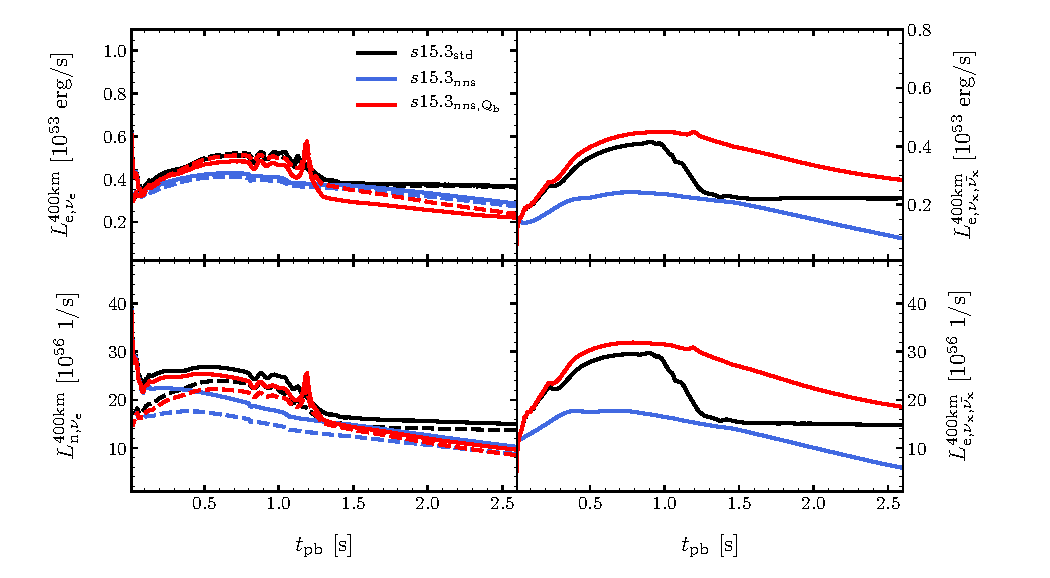
\includegraphics[width=0.8\textwidth]{./pic/s15_3_trans_tests.pdf}
\caption{Neutrino energy and number luminosities for a $15.3\,\mathrm{M_{\odot}}$ star using the transport of S06 ($s15.3_{\mathrm{std}}$), the corrected transport ($s15.3_{\mathrm{nns}}$) and including Bremsstrahlung ($s15.3_{\mathrm{std,Q_b}}$). \textit{Upper left panel}: Electron neutrino (solid lines) and electron anti-neutrino energy-luminosity at $400\,\mathrm{km}$. \textit{Lower left panel}: Electron neutrino (solid lines) and electron anti-neutrino number-luminosity at $400\,\mathrm{km}$. The left column of panels shows the same quantities for the heavy neutrinos ($\nu_{\mathrm{x}}$). Including the corrections presented here reduces the overall luminosities for this model. Adding Bremsstrahlung somewhat balances the reduction of $L_{\mathrm{e,n},\nu}$}
\label{fig:s15.3 trans}
\end{figure*}

\subsection{Bremsstrahlung}

In addition to the aforementioned improvements we now include neutrino Bremsstrahlung into our transport scheme. We follow the prescription given in \cite{Burrows2006}.
The total volumetric heating rate $ Q_{\mathrm{nb}}^{\mathrm{\nu_i}}$ by Nucleon-Nucleon Bremsstrahlung pair events, using the matter temperature $T$ and mass fractions $X_{\mathrm{n}}$, is given by

\begin{equation}
Q_{\mathrm{nb}}^{\mathrm{\nu_i}} = 0.5\cdot 1.04\cdot 10^{30} \xi \, \big(X_{\mathrm{n}}\rho_{14}\big)^2 (\frac{T}{\mathrm{MeV}})^{5.5} \,\, \Big[\frac{\mathrm{erg}}{\mathrm{cm^3s}}\Big],
\end{equation}
where $\rho_{14} = \frac{\rho}{10^{14}} \mathrm{\frac{g}{cm^3}} $
and $X_{\mathrm{n}}^2$ is defined as
\begin{equation*}
X_{\mathrm{n}}^2 = X_{\mathrm{neut}}^2 + X_{\mathrm{prot}}^2 + 28/3\, X_{\mathrm{neut}}X_{\mathrm{prot}}.
\end{equation*}

We add a factor of 0.5 in the above description as we calculate the energy generation by \textbf{one} neutrino and not by pairs of neutrinos. Here $\xi$ is a correction factor also set to 0.5.
For the energy loss $Q_{\mathrm{nb}}^{-}$ we assume
\begin{equation}
\frac{\kappa}{n_{\mathrm{b}}} = \frac{Q_{\mathrm{nb}}^{\mathrm{\nu_i}}}{c \epsilon^{\mathrm{eq}}} = \frac{Q_{\mathrm{nb}}^{-}\cdot 4\pi r^2 f_{\nu}}{L_{\nu}^{\mathrm{e}}}, 
\end{equation}
where $\kappa$ is the transport opacity as defined in S06, $n_{\text{b}}$ the baryon number density and $\epsilon^{\mathrm{eq}}$ is he mean neutrino energy assuming equilibrium conditions.
In the notation of S06 this yields
\begin{equation}
Q_{\mathrm{nb}}^{-} = \frac{Q_{\mathrm{nb}}^{\mathrm{\nu_i}} L_{\nu}^{\mathrm{e}} }{4\pi r^2 f_{\nu} c \epsilon^{\mathrm{eq}} n_{\mathrm{b}}}.
\end{equation}
For the Number emission we take
\begin{equation}
R=\frac{Q_{\mathrm{nb}}^{\nu_{\mathrm{i}}}}{\langle \epsilon \rangle} = Q_{\mathrm{nb}}^{\nu_i} \frac{L_{\nu}^n }{L_{\nu}^e }\,\, \mathrm{\frac{1}{cm^3s}}
\end{equation}
and for the absorption taking the equilibrium neutrino number density $n^{\mathrm{eq}}$ giving
\begin{equation}
n^{\mathrm{eq}} = \frac{8\pi T^3}{(hc)^3}\mathrm{F}_2.
\end{equation}
Here $\mathrm{F}_2$ is the Fermi-Dirac integral defined in Equation (D.23) in \cite{Scheck2006}.

%% TODO
%% SHOW TESTS
%% pair production should cool the material!

\section{Neutron star kicks and spin}
\label{Appendix:Neutron Star Properties}
Acceleration of neutron stars are caused by two mechanisms. 
Asphericities developing during the explosion exert gravitational forces on the PNS which accelerate the PNS in the direction opposite of the direction of the explosion. This mechanism is also known as the ``gravitational tug-boat mechanism'' \citep{Wongwathanarat2013}. For a thorough discussion of this mechanism the reader is referred to \citet{Scheck2006,Wongwathanarat2013,Janka2017,Gessner2018,Mueller2019}.
Secondly, anisotropic emission of neutrinos, specifically the anisotropic neutrino energy flux density $F_{\mathrm{\nu}}^{\mathrm{e}}$ across the surface of the PNS, exerts a force onto the PNS in the direction opposite to the stronger neutrino emission.
Using the momentum conservation equation the hydrodynamic NS kick can be simply estimated as
\begin{equation}
  \pmb{\mathrm{P}}_{\mathrm{NS}} = \pmb{\mathrm{v}}_{\mathrm{NS}}\mathrm{M_{NS}} = -\pmb{\mathrm{P}}_{\mathrm{gas}},
\end{equation}
where $\mathrm{M_{NS}}$ is the baryonic (NS) mass contained inside the radius where the angle-averaged density drops below $10^{11}\, \gcc$ and $\pmb{\mathrm{P}}_{\mathrm{gas}}\mathord{=}\int_{_{R_{\mathrm{NS}}}}^{\infty} \rho\pmb{v}\ud V$ is the momentum of the ejecta outside the PNS.
The momentum transfer by neutrinos is given by
\begin{equation}
    \label{equ:nukick}
    \dot{\textit{\textbf{P}}}_{\nu} (t) = \oint_{r = R_\mathrm{gain}}
    \frac{F_{\nu}}{c}\ \textit{\textbf{e}}_r \, \ud S
    = - \dot{\textit{\textbf{P}}}_\mathrm{ns}^{\,\nu} (t) \,.
\end{equation}
Due to the RbR approximation in \vertexprom, only radial momentum flux has
to be considered.
Assuming the PNS mass does not change significantly ($\dot{M}_{\mathrm{NS}}\mathord{=}0$), and using $\textit{\textbf{P}}_\nu (t)\mathord{=}\int_0^{\, t} \dot{\textit{\textbf{P}}}_{\nu} 
(t')\mathrm{d}t'$, the velocity of the NS can be calculated as
\begin{equation}
  \pmb{\mathrm{v}}_{\mathrm{NS}}(t) = - \frac{\pmb{\mathrm{P}}_{\mathrm{gas}} + \pmb{\mathrm{P}}_{\mathrm{\nu}}}{ \mathrm{M_{NS}}}.
  \label{equ:momentum_kick}
\end{equation}.

One can connect the asymmetry of the ejecta and neutrino emission by the means of an anisotropy parameter. The hydrodynamic parameter reads 
\begin{equation}
    \alpha_{\mathrm{NS}} = \frac{|\mathbf{P}|_{\mathrm{gas}}}{P_{\mathrm{ej}}}
\end{equation}
where 
\begin{equation}
P_{\mathrm{ej}}=\int_{R_{\mathrm{NS}}}^{R_{\mathrm{sh}}}\rho |\mathbf{v}| \ud V
\end{equation}
is the total momentum stored in the ejecta.
For the neutrino anisotropy parameter we use 
the total energy loss rate in neutrinos, which is given by
\begin{equation}
\label{nuerg}
\dot{E}_\nu (t) = \oint_{r = R_\mathrm{gain}} F_{\!\nu}\, \ud S\,.
\end{equation}
The time dependent total flux of neutrino momentum through the sphere at 
$R_\mathrm{gain}$ is given by $c^{-1}E_\nu$ and allows one to define the
instantaneous neutrino emission anisotropy parameter as
\begin{equation}
\label{nuanis}
{\widetilde\alpha}_\nu (t) = 
c\,\frac{|\dot{\textit{\textbf{P}}}_{\nu}(t)|}{\dot{E}_\nu(t)}\,.
\end{equation}
In analogy to the ejecta momentum, the momentum radiated by neutrinos is
\begin{equation}
\label{pnu}
\frac{1}{c} E_\nu (t)
= \frac{1}{c}\int_0^{\, t} \oint_{r = R_\mathrm{gain}}F_{\!\nu}\, \ud S \mathrm{d}t'
\end{equation}
so that the integral neutrino emission asymmetry at time $t$ becomes
\begin{equation}
\label{anu}
\alpha_\nu (t) = c\,\frac{|{\textit{\textbf{P}}}_{\nu}(t)|}{E_\nu(t)}\,.
\end{equation}


In addition, we compute the NS spin by integrating the flux of angular momentum through a sphere of radius $r_0\,\mathord{=}\,500\,\km$ around the origin,
\begin{equation}
    \label{equ:jns}
    \frac{\mathrm{d}\mathbf{J}_{\mathrm{NS}}}{\mathrm{dt}} = r_0^2\int_{\Omega} \rho v_r \mathbf{v}\times \mathbf{r} \mathrm{d}\Omega,
\end{equation}
where $\rho$ is the density, $\mathbf{v}$ and $\mathbf{r}$ are the vector valued velocity and position and $v_r$ the radial velocity.

In order to estimate the spin period of the PNS $P_{\mathrm{NS}}=I_{\mathrm{NS}}/|J_{\mathrm{NS}}|$, with $I_{\mathrm{NS}}$ being the moment of inertia of the PNS, we use the approximation by \citet{Lattimer2004}
\begin{eqnarray}
    I_{\mathrm{NS}} &=& 0.237M_{\mathrm{g}}R_{\text{NS}}^2\left[1 + 4.2 A  + 90 A^4\right],\\
    A &=&  M_{\text{g},\solm}R_{\text{NS},\km}^{-1},\nonumber
    \label{equ: ins}
\end{eqnarray}
where $M_{\text{g},\solm}$ is the gravitational mass of NS in units of $\solm$, and $R_{\text{NS},\km}$ is the radius of the NS in units of $\km$.
In the above equation the gravitational mass $M_{\mathrm{g}}$ can be estimated from the baryonic mass $M_{\mathrm{b}}$  as \citep{Lattimer2000}
\begin{equation}
    M_{\mathrm{g}} = M_{\mathrm{b}} - \frac{0.6 \beta}{1-0.5\beta}  M_{\mathrm{g}}, 
\end{equation}
where $\beta=\frac{GM_{\mathrm{g}}}{R_{\mathrm{NS}}c^2}$ and
$M_{\text{b},\solm}$ is the baryonic mass of the NS.

\section{Scaling relations for $Q_{\nu}$ in \vertexprom}
\label{appendix:scaling relations}

In the following the scaled Source Terms used for extending the simulations in \vertexprom are presented. The general procedure is to use the angle averaged source term for neutrino heating and cooling from the last output where the full neutrino transport was enabled. By scaling these to the contraction of the neutron star and the gain radius the relations following in the next paragraphs are derived. They are also tested and scaled against 1D simulations of the respective runs with the full neutrino transport.
\subsection{Scaling relations}
For scaling the evolution of the source terms over time the following factors are defined

\begin{align}
    g(t) &= \frac{L_{\nu_e}(t) +          L_{\bar{\nu}_e}(t)}{L_{\nu_e}(t_0) +
    L_{\bar{\nu}_e}(t_0)}, \\
    h(t) &= \left(\frac{E_{\nu_e}(t) + E_{\bar{\nu}_e}(t)}{E_{\nu_e}(t_0) +
    E_{\bar{\nu}_e}(t_0)}\right)^2,
\end{align}
where $L_{\mathrm{\nu_e}}, \;L_{\mathrm{\bar{\nu}_e}}$ are the electron neutrino and anti-neutrino luminosities at time $t$ and initial time $t_0$. $E_{\mathrm{\nu_e}}, \;E_{\mathrm{\bar{\nu}_e}}$ are the neutrino energies. With these we define

\begin{align}
    F_\mathrm{gain}(t) &=
    \left(\frac{R_\mathrm{gain}(t_0)}{R_\mathrm{gain}(t)}\right)^2 , \\
    F_\mathrm{E}(t) &= h(t)
    \left(\frac{M_\mathrm{NS}(t)}{M_\mathrm{NS}(t_0)}\right)^2 , \\
    \Gamma(t) &= \frac{M_\mathrm{NS}(t) \,\dot{M}(t)
    \,R_\mathrm{NS}(t_0)}{M_\mathrm{NS}(t_0) \,\dot{M}(t_0) \,R_\mathrm{NS}(t)} , \\
    F_{\dot{M}}(t) &= \frac{\frac{1}{2} L_{\nu_x}^\mathrm{tot}(t_0) \,g(t) + \left[
    L_{\nu_e+\bar{\nu}_e}(t_0) - \frac{1}{2} L_{\nu_x}^\mathrm{tot}(t_0)
    \right] \Gamma(t)}{L_{\nu_e+\bar{\nu}_e}(t_0)}.
\end{align}

In order to calculate the mass accretion rate $\dot{M}$, we only integrate fluid elements with $v_r < 0$ at $r = 100$~km.
For the low mass iron cores models \znine and \snine we set

\begin{align}
    L_{\nu_e+\bar{\nu}_e}(t_0) &= \frac{1}{2} L_{\nu_x}^\mathrm{tot}(t_0) \\
    \Rightarrow F_{\dot{M}}(t) &\equiv g(t)
\end{align}

In order to incorporate the contraction of the gain radius we define
\begin{align}
    x &= \frac{r(t)}{R_\mathrm{gain}(t)} \\
    \Rightarrow r(t) &= r(t_0) \frac{R_\mathrm{gain}(t)}{R_\mathrm{gain}(t_0)}
\end{align}
where $R_{\mathrm{gain}}(t)$ is defined later on.



Outside the neutron star we apply the heating terms for energy and lepton number as

\begin{align}
    Q_\mathrm{erg}(r) &= \frac{Q_\mathrm{erg}^0}{\rho_0}(x) \,\rho (r)
    \,F_{\dot{M}} \,F_\mathrm{E} \,F_\mathrm{gain} , \\
    Q_\mathrm{lep}(r) &= \frac{Q_\mathrm{lep}^0}{\rho_0}(x) \,\rho (r)
    \,F_{\dot{M}} \,F_\mathrm{E} \,F_\mathrm{gain} \,\mathrm{sign}(v_r)
\end{align}
The corresponding cooling terms over the whole domain are defined as 

\begin{align}
    Q_\mathrm{erg}(r) &= \frac{Q_\mathrm{erg}^0}{\rho_0}(x) \,\rho (r)
    \,\left[\frac{T(r)}{T_0(r)}\right]^6 , \\
    Q_\mathrm{lep}(r) &= \frac{Q_\mathrm{lep}^0}{\rho_0}(x) \,\rho (r)
    \,\left[\frac{T(r)}{T_0(r)}\right]^5 \, \mathrm{max}\left\{0, \frac{Y_e(r) -
    0.01}{Y_e^0(r) - 0.01}\right\} %\\
\end{align}

Note that heating applies only if $r > R_\mathrm{NS}$ and $Q_\mathrm{erg/lep}^0 (x) > 0$, whereas cooling is applied within the neutron star and if $Q_\mathrm{erg/lep}^0 (x) < 0$.

For the \znine and \snine we set
\begin{align}
    Q_\mathrm{erg}(r) &= \frac{Q_\mathrm{erg}^0}{\rho_0^2}(x) \,\rho^2 (r)
    \,\left[\frac{T(r)}{T_0(r)}\right]^6 ,\\
    Q_\mathrm{lep}(r) &= \frac{Q_\mathrm{lep}^0}{\rho_0^2}(x) \,\rho^2 (r)
    \,\left[\frac{T(r)}{T_0(r)}\right]^5 \, \mathrm{max}\left\{0, \frac{Y_e(r) -
    0.01}{Y_e^0(r) - 0.01}\right\} \\
\end{align}


When the initial mass accretion rate as defined earlier is greater than zero the gain radius scales as

\begin{align}
    C_0 &= \frac{R_\mathrm{gain}(t_0)}{R_\mathrm{NS}(t_0)}, \\
    b &= \mathrm{min} \left\{1.01, C_0 \right\}, \\
    R_\mathrm{gain}(t) &= \left[ \left( C_0 - b \right)
    \frac{\dot{M}(t)}{\dot{M}(t_0)} + b \right] \,R_\mathrm{NS}(t)
    \label{eq:1}
\end{align}

Should there be no accretion and to avoid dividing by zero in Eq.~(\ref{eq:1}),  we use

\begin{equation}
    R_\mathrm{gain}(t) = b \, R_\mathrm{NS}(t).
\end{equation}

\subsection{Neutrino pressure correction}

Since switching off the neutrino transport also turns off the calculation of the supporting neutrino pressure we use the analytic formula

\begin{equation}
    p_{\nu} = \frac{4 \pi (k T)^4}{3 (h c)^3} \left[ \frac{21
    \pi^4}{60} + \frac{1}{2} \eta^2 \left( \pi^2 + \frac{1}{2} \eta^2 \right)
    \right]
\end{equation}

The neutrino pressure correction  term $p_{\nu} \cdot F_p(\rho)$ is added to the gas pressure in the equation of state and to the general-relativistic gravitational potential.

In the above equations we use
\begin{align}
    \eta &= \frac{\mu_{\nu} - (m_n - m_p) c^2}{k T} \\
    F_p(\rho) &= \frac{p_\mathrm{vertex}(\rho,t_0)}{p_{\nu}(\rho,t_0)} \mathrm{min}\left\{ 1, \frac{\rho}{10^{13}\,\mathrm{g/cm^3}} \right\} \\
    p_\mathrm{vertex} &= \frac{4\pi}{c} \sum_{\nu} \int \mathrm{d}\epsilon \,
    J(\nu,\epsilon) \, \mathrm{max}\left\{ \frac{1}{3},  f_K(\nu,\epsilon) \right\}
\end{align}
where $\mu_{\nu}$ is the neutrino chemical potential and $p_{\mathrm{vertex}}$ the numerical neutrino pressure term of \vertexprom.

\newpage

\label{lastpage}
\end{document}
% end of file template.tex

